%%%%%%%%%%%%%%%%%%%%%%%%%%%%%%%%%%%%%%%%%%%%%%%%%%%%%%%%%%%%%%%%%
%  _____       ______   ____									%
% |_   _|     |  ____|/ ____|  Institute of Embedded Systems	%
%   | |  _ __ | |__  | (___    Wireless Group					%
%   | | | '_ \|  __|  \___ \   Zuercher Hochschule Winterthur	%
%  _| |_| | | | |____ ____) |  (University of Applied Sciences)	%
% |_____|_| |_|______|_____/   8401 Winterthur, Switzerland		%
%																%
%%%%%%%%%%%%%%%%%%%%%%%%%%%%%%%%%%%%%%%%%%%%%%%%%%%%%%%%%%%%%%%%%


% The ZHAW INES latex style scrip
\documentclass{clsFile/zhawines}

% Command redefinitions

% To use new glossaries package uncomment this line. This requires Perl to be installed on the computer (http://strawberryperl.com/)
% Comment this line if you want to use the old manual glossary (see file /content/glossar)
%\newcommand*{\USEGLOSSARIES}{} 

%Include your own packages that are needed for you document, here the packages for the example are added
\usepackage{scrlayer-scrpage}
\usepackage{listings}
\usepackage{amsmath}
\usepackage[squaren]{SIunits}
\usepackage{graphicx}
\usepackage{array}
\usepackage{float}
\usepackage{pbox}
\usepackage{caption}
\ifdefined\USEGLOSSARIES
	\usepackage[acronyms]{glossaries}
	\makeglossaries
	%%%%%%%%%%%%%%%%%%%%%%%%%%%%%%%%%%%%%%%%%%%%%%%%%%%%%%%%%%%%%%%%%
%  _____       ______   ____									%
% |_   _|     |  ____|/ ____|  Institute of Embedded Systems	%
%   | |  _ __ | |__  | (___    Wireless Group					%
%   | | | '_ \|  __|  \___ \   Zuercher Hochschule Winterthur	%
%  _| |_| | | | |____ ____) |  (University of Applied Sciences)	%
% |_____|_| |_|______|_____/   8401 Winterthur, Switzerland		%
%																%
%%%%%%%%%%%%%%%%%%%%%%%%%%%%%%%%%%%%%%%%%%%%%%%%%%%%%%%%%%%%%%%%%

% Glossary Eintraege
\newglossaryentry{akronym}{name=akronym,plural=akronyme, description={Ein Akronym ist ein aus den Anfangsbuchstaben mehrerer Wörter gebildetes Kurzwort}}


% Akronym Eintraege
\newacronym{zhaw}{ZHAW}{Zürcher Hochschule für Angewandte Wissenschaften}
\newacronym{ines}{InES}{Institute of Embedded Systems}
\newacronym{tofcamera}{TOF Camera}{Time of Flight Camera}
\newacronym{fpga}{FPGA}{Field Programmable Gate Array}
\newacronym{pcie}{PCIe}{PCI Express}
\newacronym{pci}{PCI}{Peripheral Component Interconnect}
\newacronym{usb}{USB}{Universal Serial Bus}
\newacronym{CSI}{CSI}{Camera Serial Interface}


\fi

\DeclareCaptionFormat{myformat}{#1#2#3\hrulefill}
\captionsetup[figure]{format=myformat}

\begin{document}
%How the hyperlinks are shown, remove this or change it if you want the colorful links
\hypersetup{
    colorlinks = false,
    urlbordercolor = {1 1 1},
    linkbordercolor = {white},
}

%Select language, all generated content will be in the selected language
\selectlanguage{english} %possible german/english

% Generate your title page, it takes the arguments author, title
% and email. The title page is then generated with maketitle
\author{Marcel Wegmann \newline }
\title{Vulkan-CUDA Co-Design for Real-Time Object Classification}
\email{wegr@zhaw.ch}
\newcommand{\version}{1.0}

% Add Copyright informations and Contact infos
 \newcommand{\confidential}{no}  %write yes to have a confidential mark on every normal page

\maketitle


% Generate the header and footer of the document
\headings

% Stop page numbering for abstract and anti-plagiarism statement
\pagenumbering{gobble}

% Include anti-plagiarism statement. The Word template is located in the same folder

\includepdf[scale=0.9,pages=1]{pdf/plagiatserklaerung.pdf}

% Include abstract
%!TEX root = ../doc.tex

\chapter*{Abstract}
\label{sec:Abstract}
Augmented Reality is the concept of enhancing the real world with virtual objects or information with projections into a viewfinder or through specialized goggles. Simpler forms of Augmented Reality – like a heads-up display in a car – do not need to estimate the camera's motion, an object, or the user.  However, more elaborate implementations of Augmented Reality need to track things and, more importantly, the camera's movement itself. The applications in which Augmented Reality could be leveraged range from social interaction over pedestrian navigation to various use cases in different professions. Multiple companies already have shown closed source or custom-tailored programming interfaces, either running on smartphones or shipped with industry-targeted goggles. The tracking of real-world objects surfaces or is possible with the provided interfaces, but the algorithms behind the different functions are corporate secrets.\\ 
This thesis describes an approach for an end-to-end pipeline in a prototype of an Augmented Reality platform without using commercial interfaces. A time-of-flight camera provides a depth image that allows reconstruction of the recorded scene as a cloud of SIFT features. Frame-by-frame analysis of the point cloud estimates the camera's motion by highly parallel processing and a three-dimensional extension of the RANSAC algorithm. An accelerometer and a gyroscope provide additional data, fused with a Kalman filter to improve the motion estimation. A regular color camera acts as a viewfinder, and Vulkan renders the result to a monitor.\\
Enhancing the matching quality of SIFT features between consecutive frames of a time-of-flight camera using a three-dimensional RANSAC algorithm led to over two times as many correct matches. Despite noisy camera data, the estimation of the camera rotation and translation of the time-of-flight camera based on these matches works as demonstrated in the thesis. The sensor fusion with the Kalman filter works as intended for rotations. Still, it fails for translations because of the system's low sampling rate and the accelerometer's hysteresis, failing to compensate appropriately for gravity.

\chapter*{Preface}
\label{sec:Vorwort}
I am thankful to my supervisor, Prof. Dr. Matthias Rosenthal, for allowing this deep dive into Augmented Reality and the support given during this thesis. Furthermore, I am grateful for the support and advice from the ZHAW InES HPMM team.\\Special thanks, especially to Lukas Neuner, for his valuable inputs during this thesis and for proofreading this document. Additional thanks are given to Alexey Gromov for his support in setting up the Jetson Xavier and proofreading this document. I am thankful for the chance of gaining further experience in CUDA, Vulkan and for the time given to learn new topics in the math involved in three-dimensional rendering. \\
In addition, I thank all my friends and family members for giving support and motivation. 

% Start page numbering
\pagenumbering{arabic}

%Include table of content
\tableofcontents

% Starts the page count from here, pdf viewers will be able to jump to the corret page.
\setcounter{page}{1}

%Include all chapters. Chapters itself are in the content subfolder
% %%%%%%%%%%%%%%%%%%%%%%%%%%%%%%%%%%%%%%%%%%%%%%%%%%%%%%%%%%%%%%%%%
%  _____       ______   ____									%
% |_   _|     |  ____|/ ____|  Institute of Embedded Systems	%
%   | |  _ __ | |__  | (___    Wireless Group					%
%   | | | '_ \|  __|  \___ \   Zuercher Hochschule Winterthur	%
%  _| |_| | | | |____ ____) |  (University of Applied Sciences)	%
% |_____|_| |_|______|_____/   8401 Winterthur, Switzerland		%
%																%
%%%%%%%%%%%%%%%%%%%%%%%%%%%%%%%%%%%%%%%%%%%%%%%%%%%%%%%%%%%%%%%%%

\chapter{LaTeX Kurzanleitung}\label{chap.anleitung}
Dieses Kapitel führt mit Beispielcode in den LaTeX Code ein, und kann während der Erstellung des Dokuments gelöscht werden.\footnote{Verbesserungsvorschläge bitte an hegt@zhaw.ch senden}

Die nachfolgende Berichtstruktur wurde aus der Vorlage\footnote{Berichtstruktur Vorlage, Stand: August 2011} der \href{https://intra.zhaw.ch/departemente/school-of-engineering/studium-standort-winterthur/studierende/projektarbeit-bachelorarbeit.html}{PA/BA Termin-Webseite} vom ZHAW Intranet entnommen.

(): alle in Klammer aufgeführten Einträge sind situativ anzupassen



Das ist ein kleiner Text um zu zeigen, wie die Enter eingebracht werden.\\
Ich finde Latex schwierig.\\
Der Start ist echt eine Herausforderung. \\
Mensch ist das Komplex, echt was für Profis. % Hier brauchts ja kein Enter mehr, sonnst heisst es Overfull \hbox



\section{Visio Vektorgraphik einfügen}\label{visio}
(Graphik auswählen) Speichern unter -> PDF -> Optionen.. -> Auswahl\\
Mit Adobe Akrobat öffnen: Erweitert -> Druckproduktion -> Seiten beschneiden -> Weisse Ränder entfernen -> OK -> Ctrl-S

\begin{figure}[H]
	\centering
		\includegraphics[width=0.8\textwidth]{images/visio/visio.pdf}
	\caption{Ideenskizze}
	\label{fig.Skizze}
\end{figure}

So kann die Abbildung~\ref{fig.Skizze} referenziert werden. Bei der PDF Erstellung ist darauf zu achten, dass LaTeX nur Versionen bis 1.4 voll unterstützt. 



\subsection{Graphiken in LaTeX zuschneiden}\label{zuschneiden}
Mit dem Befehl Clip kann eine Graphik auch in LaTeX zugeschnitten werden:

\begin{figure}[H]
	\centering
		\includegraphics[width=0.9\textwidth, clip=true, trim = 80 10 0 10]{images/visio/visio.pdf}  % trim lm bm rm tm (left, bottom, right, top)
	\caption{clip=true, trim = 60 10 0 10}
	\label{fig.SkizzeZugeschnitten}
\end{figure}



\subsection{Mehrere Bilder nebeneinander}\label{nebeneinander}
Dank Minipages können mehrere Bilder auch nebeneinander sein:

%Zwei Bilder nebeneinander http://latex.mschroeder.net/
\begin{figure}[H]
  \centering
  \begin{minipage}[b]{0.45\textwidth}
    \includegraphics[scale=0.15]{images/photoshop/Skizze.jpg}
    \caption{Visir10b Detector}
    \label{Visir10bDetector} 
  \end{minipage} % Hier darf keine Leerzeile zwischen den beiden Minipages liegen!
  \begin{minipage}[b]{0.45\textwidth}
    \includegraphics[scale=0.15]{images/photoshop/Skizze.jpg} 
    \caption{Visir10b Model}
    \label{Visir10bModel} 
  \end{minipage}
  \caption{Visir 10 mit optimiertem Reflektor}
  \label{fig.Visir10b}
\end{figure}


Literaturverweis: \citep{analog_devices_dac} \citep{microchip_spi}

\section{Tabellen aufbauen}\label{tabelle}
Kleine Tabelle:

\begin{table}[ht] \centering
	\begin{tabular}{|p{3cm}|p{.5cm}|p{.5cm}|p{.5cm}|p{.5cm}|p{.5cm}|p{.5cm}|p{.5cm}|p{.5cm}|p{.5cm}|p{.5cm}|} \hline
		\rowcolor{gray} Modul & M01 & M02 & M03 & M04 & M05 & M06 & M07 & M08 & M09 & M10 \\
		\hline
		FPGA\_DATEN & & & & & X & X & & X & X & \\
		\hline
		IRQ & X & X & X & & X & & & & X & X \\
		\hline
		Nachbar Core & & & & X & & X & & X & & \\
		\hline
	\end{tabular}
	\caption{Port Schwierigkeiten der Funkmodule}
	\label{tab:portprobleme}
 \end{table}	

Die nachfolgende longtable kann sich über mehrere Seiten erstrecken.

\begin{longtable}{|p{1.1cm}|p{4cm}|p{4cm}|p{4cm}|} 
					\hline
					\rowcolor{gray} Typ & Variante A & Variante B & Variante C
					\\ \hline
					& \textbf{Vorteile:} 
							\begin{itemize}
								\item[+] hohe Spannungen
							\end{itemize}							
							\textbf{Nachteile:}
							\begin{itemize}
								\item[-] Grosse Abmessung
							\end{itemize}
					& 	\textbf{Vorteile:} 
							\begin{itemize}
								\item[+] einfache Montage
							\end{itemize}							
							\textbf{Nachteile:}
							\begin{itemize}
								\item[-] max. 2A Eingangsstrom
							\end{itemize}
					&	\textbf{Vorteile:} 
							\begin{itemize}
								\item[+] hoher Strom
							\end{itemize}							
							\textbf{Nachteile:}
							\begin{itemize}
								\item[-] max. 12 V Eingangsspannung
							\end{itemize}\\ \hline
						Zeit & 2 h & 5 h & 3 h \\ \hline
						Preis	& 520 CHF/Stück & 800 CHF/Stück &	360 CHF/Stück\\ \hline
				\caption{Morphologischer Kasten für die Speisung}
				\label{tab:morphkasten}
			\end{longtable}	

Diese Art von Tabelle erstreckt sich immer auf der ganzen Seitenlänge:

\begin{tabularx}{\textwidth}{XXl}
  Salat & Schnecke & Igel\\
  Montag & Hier ist ein langes Wort & Dienstag
\end{tabularx}



\section{Code Listings aufbauen}\label{listing}

\begin{lstlisting}[
    language=C++,
    caption={Test Kommandozeilen Ausgabe},
    label={list.Testoutput}
]
/********************************************************/
/* Name        : M07Setup                               */
/* Description : EM9201 init for adress and pck         */
/* Input       : targetadr (DevAdr_M00 - DevAdr_M39)    */
/*               drate (Drate_M00 - Drate_M39)          */
/* Ouput       : -0x01 -> Setup OK                      */
/*               -0x5E -> Setup Error Channel write     */
/*               -0x6E -> Setup Error power write       */
/*               -0x7E -> Error in Device Address       */
/*               -0x8E -> Error in Peer Address         */
/********************************************************/
\end{lstlisting}

Formula $e = \sqrt{a{^2} - b^{2}}$


Diese Textstelle ist sehr interessant.\label{interessant}\\
Hier wird auf die Textstelle~\ref{interessant} verwiesen, die sich auf der Seite~\pageref{interessant} befindet.




\section{Citation nach IEEE}\label{citation}

Das ist ein \cite{analog_devices_dac} Verweis aufs Literaturverzeichnis. Ein anderes Beispiel ist das hier \cite{mirrorcle_userguide}.





Das ist eine Aufzählung:
\begin{itemize} %
	\item Erste Zeile
	\item Zweite Zeile
	\item Dritte Zeile
\end{itemize}


\begin{enumerate}
\item erstens
\item zweitens
\end{enumerate}

%https://parma.zhaw.ch/svn/zhw_latex/
%gmanstyle nötig unter start od begin einbinden


Das ist eine verschachtelte Aufzählung:
\begin{description}
		\item [Register Performance] Alle Signale die das FPGA nicht verlassen, also von FF zu FF weitergeleitet werden. Daraus ergibt sich die maximale Taktfrequenz F\textsubscript{MAX}.

		\item [Externes Timing] FPGA Ein- und Ausgänge
		\begin{itemize}
			\item Ausgänge = Von FF's durch Logik zu Ausgängen (t\textsubscript{CO})
			\item Eingänge = Von Eingängen durch Logik zu FF's (t\textsubscript{SU}, t\textsubscript{H})
			\item Durchgänge = kombinatorische Pfade durch das FPGA (t\textsubscript{PD})
		\end{itemize}
\end{description}

\ifdefined\USEGLOSSARIES

	\section{Akronyme und Glossar}\label{acronymsandglossaries}
	
	\subsection{Akronyme}\label{acronymsandglossary.acronyms}
	Ein Akronym ist ein aus den Anfangsbuchstaben mehrerer Wörter gebildetes Kurzwort. 
	
	
	Einträge der Akronyme können im Text folgendermassen dargestellt werden:
	\begin{itemize}
		\item Das \acrshort{ines} ist Teil der \acrshort{zhaw}.
		\item Das \acrlong{ines} ist Teil der \acrlong{zhaw}.
		\item Das \acrfull{ines} ist Teil der \acrfull{zhaw}.
	\end{itemize}
	
	\subsection{Glossar}\label{acronymsandglossary.glossaries}
	Das Glossar ist eine Liste erklärungsbedürftiger und für die Arbeit
	relevanter Begriffe zusammen mit den zugehörigen Erklärungen oder
	Übersetzungen.
	
	
	Einträge des Glossars können im Text folgendermassen dargestellt werden:
	\begin{itemize}
		\item \textbf{\gls{akronym}}: Singular mit Kleinbuchstaben
		\item \textbf{\Gls{akronym}}: Singular, erster Buchstabe gross
		\item \textbf{\glspl{akronym}}: Plural mit Kleinbuchstaben
		\item \textbf{\Glspl{akronym}}: Plural, erster Buchstabe gross
	\end{itemize}

\fi


 % Remove for final document
%!TEX root = ../doc.tex
\chapter{Introduction}
\label{sec:Introduction}
Augmented Reality - or AR – is the concept of projecting virtual objects into the real world. Phone screens, tablet computers, and specialized goggles render virtual objects over the camera image or display them on translucent screens. A form of Augmented Reality is a heads-up display, for example, in cars to project the current speed and navigation information to the windshield or in airplanes for comprehensive avionic information.\\
In contrast, Virtual Reality – or VR – limits itself to entirely virtual worlds, into which the user dives. While Virtual Reality is already readily available through off-the-shelf goggles, which lets users meet other people and play games in virtual worlds, Augmented Reality is mainly limited to smartphone applications. Currently, it lacks readily available and specialized hardware, other than niche products specialized for specific industries.\\
Augmented Reality faces numerous technical challenges. Projecting a virtual object – for example, a flowerpot – into the real world requires the system to recognize a table and find an unoccupied location. Apart from placing decoration or furniture, a pair of Augmented Reality goggles could project helpful information into the air. A mechanic could have virtual schematics or instructions floating beside his work, while another virtual monitor displays a video phone call with the customer. Hand detection and gesture control would enable interaction with virtual objects. Another example could be pedestrian navigation, projecting arrows to the street. \\
AR goggles need to react in real-time to any motion of the user’s head. Any latency would break immersion as virtual objects lose the connection with their anchor point in the real world. A flowerpot would jump on the table, and arrows on the street would start to float and collide with walls. Fast and reliable motion tracking of the system itself is vital for avoiding visual glitches.
\section{Initial Situation}
\label{sec:Situation}
Multiple consulting companies like Deloitte and KPMG described virtual, augmented, and extended reality as possibly the biggest source of digital disruption since the smartphone\cite{KPMG_on_AR} and the next big thing of the digital environment\cite{Deloitte_on_AR}.\\
While Augmented Reality platforms already exist in consumer products, the know-how is developed within the walls of multi-billion tech companies like Apple or Microsoft. According to Bloomberg, Facebooks Augmented Reality and Virtual Reality, and hardware teams account for more than 6000 employees\cite{Bloomberg_on_AR}. \\
The most advanced hardware available today is the Microsoft HoloLens\cite{Hololens} featuring four cameras for motion tracking, two infrared cameras for eye-tracking, a time-of-flight sensor for depth measurement, a 9-Axis IMU (Accelerometer, Gyroscope, and Magnetometer), and an additional camera for photos and recording videos. Microsoft targets a professional environment with the Holo Lens, for example, to support Airbus technicians at maintenance\cite{AirbusHololens}.\\
The Implementation of how these sensors are fused for generating a smooth experience is closed source.\\
Other than the HoloLens, there exist numerous applications on Smartphones and Tablets running either Android, iOS, or iPadOS. Google ARCore implementation relies on Machine Vision and can benefit from – but does not require –  a ToF camera. ARCore detects objects, estimates their size, tracks objects, and finds flat surfaces. The analysis of light sources allows a virtual object to cast a realistic shadow. Apple’s counterpart is ARKit, which leverages machine learning hardware on their $Bionic$ SoCs and the LiDaR sensors used in iPads and iPhones.\cite{AppleLidar}\\
Next to these two, numerous open-source projects focus on specific do-it-yourself projects and, for example, enable AR capabilities in a web browser through JavaScript\cite{ar_js}\cite{argon_js}. 
\section{Motivation}
\label{sec:Motivation}
While advanced solid-state LiDaR scanners used in consumer products were not available on the open market in finished modules, time-of-flight cameras get marketed directly. Multiple companies sell time-of-flight cameras for industrial processes or on evaluation boards for development. Building a prototype becomes viable with off-the-shelf time-of-flight cameras and powerful embedded devices, like the Nvidia Jetson series. 
With the availability of time-of-flight cameras, it becomes worthwhile investigating the possibilities they offer for motion detection and if the acquired data could be helpful in an Augmented Reality system. 

\section{Scope}
\label{sec:Scope}
This thesis focuses on close-to-hardware fundamentals and omits the implementation of end-user applications. Without solid motion tracking of the Augmented Reality system, all the other parts of Augmented Reality fail. Developing specialized goggles is pointless without reliable motion tracking; this also falls out of the scope.
\section{Goals}
\label{sec:Goals}
The goals of the thesis are to set up an end-to-end pipeline from data recording over processing to rendering, involving a three-dimensional object which follows the motion of a camera. An off-the-shelf time-of-flight (ToF) camera delivers depth information from which the camera motion is estimated. A sensor fusion approach will combine the estimated camera motion with an IMU.

\section{Target audience}
\label{sec:Ziel}
This document is targeted at readers with a basic understanding of computer science and computer vision. Prior knowledge in linear algebra is beneficial.
%!TEX root = ../doc.tex
\chapter{Concept}
\label{sec:Concept}


%!TEX root = ../doc.tex
\chapter{Fundamentals}
\label{sec:Fundamentals}
The following chapter describes methods and technologies that are used within this thesis.
\section{3D Cameras}
\label{sec:ToFCamera}
In the field of 3D mapping, two expressions often get mentioned: LiDaR sensors and ToF cameras. As the basic principle in both technologies relies on measuring the Time of Flight (ToF) and is in both cases Light-Detection and Ranging, both expressions are ambivalent.\\
A LiDaR sensor is often referred to work together with a moving laser, that scans its surroundings.\cite{Techradar_Lidar} The mechanical mounting of such a device is too bulky to be embedded in a modern smartphone, which is why solid-state LiDaR sensors are used. A solid-state LiDaR sensor projects a grid of laser dots onto the scene, as seen in image \ref{im:iPadLidar}. The time of flight for each dot is measured individually.
\begin{figure}[H]
    \centering
    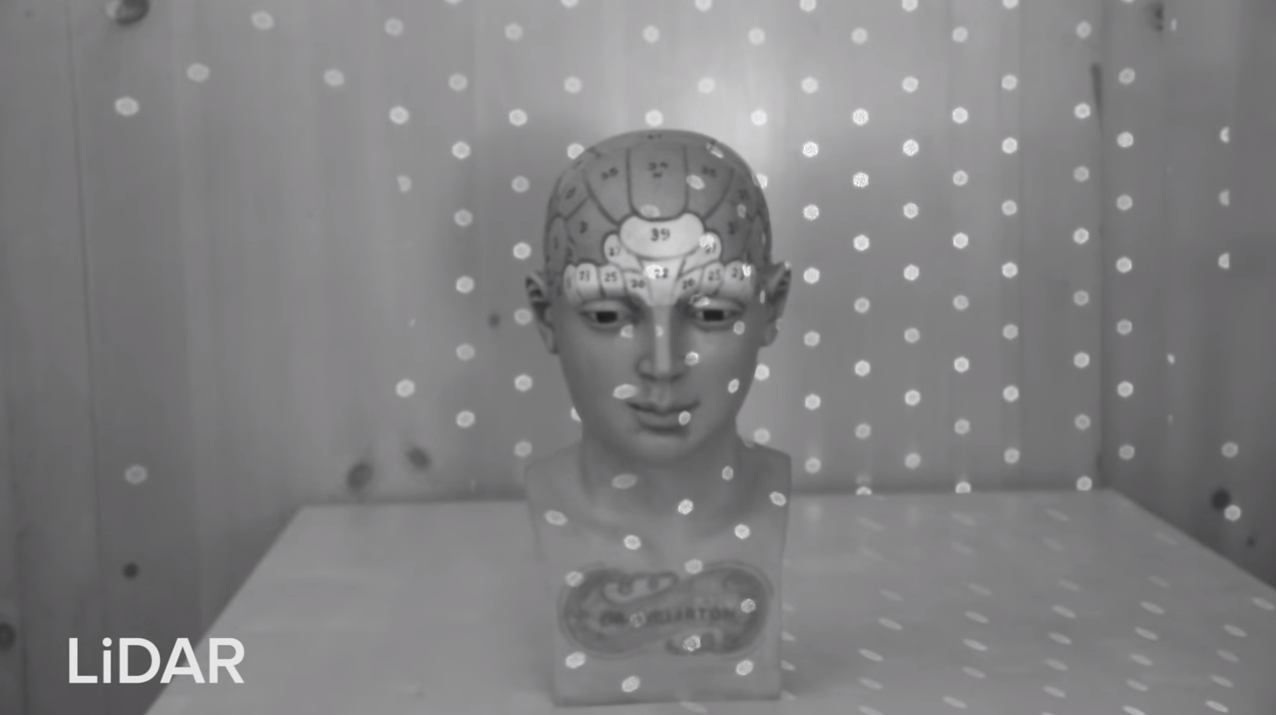
\includegraphics[width=1.0\textwidth]{images/ifixit_lidar.png}
    \caption{Projected dots from the LiDaR scanner of an Apple iPad Pro 2020, made visible with an infrared camera. Image source: iFixit.com}
    \label{im:iPadLidar}
\end{figure}
Another method for 3d mapping is, using one wide area infrared flash and measuring the time of flight on each individual sensor pixel. This approach in contrast is often referred to be a ToF camera. ToF cameras are used by different manufacturers of Android powered smart phones.\\
While the measurement principle in both technologies is the same, the LiDaR scanner generates a point cloud, while the ToF camera outputs a depth map image. With mathematical transformations, both outputs are equivalent. Another difference is that a ToF camera can double as a grayscale infrared camera, providing an image by itself. \\
The sensor used for this thesis follows the principle of a ToF camera. The measured radial distance from the sensor for each pixel allows the three dimensional reconstruction of the scene. 
\subsection{Radial information from ToF cameras}
The used ToF camera provides the measured distance from the sensor to the filmed object for each pixel, generating a depht map. Because of the radial measurement, flat surfaces appear warped. The distortion follows a curve which can be corrected by knowing the cosine of the angle $\alpha$ for each pixel.
\begin{figure}[H]
    \centering
    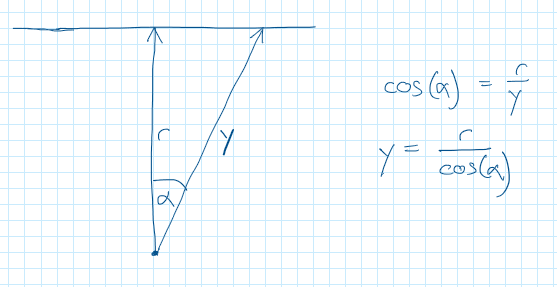
\includegraphics[width=0.5\textwidth]{images/dummy_radial_angle.png}
    \caption{Geometrics of the radial measurement and its correction.}
    \label{im:RadialCorrection}
\end{figure}
With the angle of the individual pixels being unknown, a map of cosine $\alpha$ is generated by taking an image of a flat surface.
\section{Mathematics for Rotation and Translation}
\label{sec:LinAlgRotation}
Augmented reality relies on having accurate positional and angular information to estimate the required size and warp of a virtual object projected into the real world. A MEMS module containing a gyroscope and an accelerometer provides rotation and acceleration information to the system to assist the positional tracking.
\subsection{Euler Rotations and Linear Algebra}
A common way to calculate rotations and translations are matrix-vector multiplications. The standard matrices for rotating with the angle $\phi$ around $X$, $Y$ and $Z$ are shown in the following:
\begin{equation*}
    A_{rot,X} =
    \begin{bmatrix}
        1 & 0        & 0         \\
        0 & cos \phi & -sin \phi \\
        0 & sin \phi & cos \phi
    \end{bmatrix}
    \quad
    A_{rot,Y} =
    \begin{bmatrix}
        cos \phi  & 0 & sin \phi \\
        0         & 1 & 0        \\
        -sin \phi & 0 & cos \phi
    \end{bmatrix}
    \quad
    A_{rot,Z} =
    \begin{bmatrix}
        cos \phi  & sin \phi & 0 \\
        -sin \phi & cos \phi & 0 \\
        0         & 0        & 1
    \end{bmatrix}
\end{equation*}
A combination of the three matrices leads to a rotation matrix with a rotation axis that is not strictly bound to $X$, $Y$, or $Z$. Matrix multiplication is not commutative, so the order of the multiplications matters. In the following example, the vector gets rotated first around $X$, then $Y$, and around $Z$ in the end. This chain of matrix operations is read from right to left in the equation.
\begin{equation*}
    A_{rot} =
    \begin{bmatrix}
        a_{0,0} & a_{0,1} & a_{0,2} \\
        a_{1,0} & a_{1,1} & a_{1,2} \\
        a_{2,0} & a_{2,1} & a_{2,2}
    \end{bmatrix}
    =A_{rot,Z} \cdot A_{rot,Y} \cdot A_{rot,X}
\end{equation*}
With this matrix, a three dimensional vector can be rotated at once around an arbitrary axis for the desired angle. Applying this transformation to each vertex of a virtual 3D object results in a rotation of the whole object around the origin $(0,0,0)$.\\
\begin{equation*}
    \begin{pmatrix}
        x' \\
        y' \\
        z'
    \end{pmatrix}
    =
    \begin{bmatrix}
        a_{0,0} & a_{0,1} & a_{0,2} \\
        a_{1,0} & a_{1,1} & a_{1,2} \\
        a_{2,0} & a_{2,1} & a_{2,2}
    \end{bmatrix}
    \cdot
    \begin{pmatrix}
        x \\
        y \\
        z
    \end{pmatrix}
\end{equation*}
To avoid using an inhomogenous linear system for moving an object, a fourth dimension is needed. By extending the vectors with a $1$ and using the fourth column in the matrix to alter $X$, $Y$ and $Z$, these vector entries can be moved without applying any rotation.
\begin{equation*}
    \begin{pmatrix}
        x+\Delta X \\
        y+\Delta Y \\
        z+\Delta Z \\
        1
    \end{pmatrix}
    =
    \begin{pmatrix}
        x' \\
        y' \\
        z' \\
        1
    \end{pmatrix}
    =
    \begin{bmatrix}
        1 & 0 & 0 & \Delta X \\
        0 & 1 & 0 & \Delta Y \\
        0 & 0 & 1 & \Delta Z \\
        0 & 0 & 0 & 1
    \end{bmatrix}
    \cdot
    \begin{pmatrix}
        x \\
        y \\
        z \\
        1
    \end{pmatrix}
\end{equation*}
To combine the rotation matrix with the translation matrix, the 3x3 rotation matrix gets placed top-left into the 4x4 unit matrix. Now, the rotation matrix also being a 4x4 matrix, rotations and translations can be chained up following the common laws of linear algebra. Chaining up translations and rotations allows moving the rotation axis for an object.
\begin{equation*}
    \begin{pmatrix}
        x' \\
        y' \\
        z' \\
        1
    \end{pmatrix}
    =
    \begin{bmatrix}
        a_{0,0} & a_{0,1} & a_{0,2} & 0 \\
        a_{1,0} & a_{1,1} & a_{1,2} & 0 \\
        a_{2,0} & a_{2,1} & a_{2,2} & 0 \\
        0       & 0       & 0       & 1
    \end{bmatrix}
    \cdot
    \begin{pmatrix}
        x \\
        y \\
        z \\
        1
    \end{pmatrix}
\end{equation*}
The dependency on the order of the rotations poses a problem visualized in image \ref{im:EulerRotation}: The values returned by a gyroscope would need to be applied all at once and not one after another.
\begin{figure}[H]
    \centering
    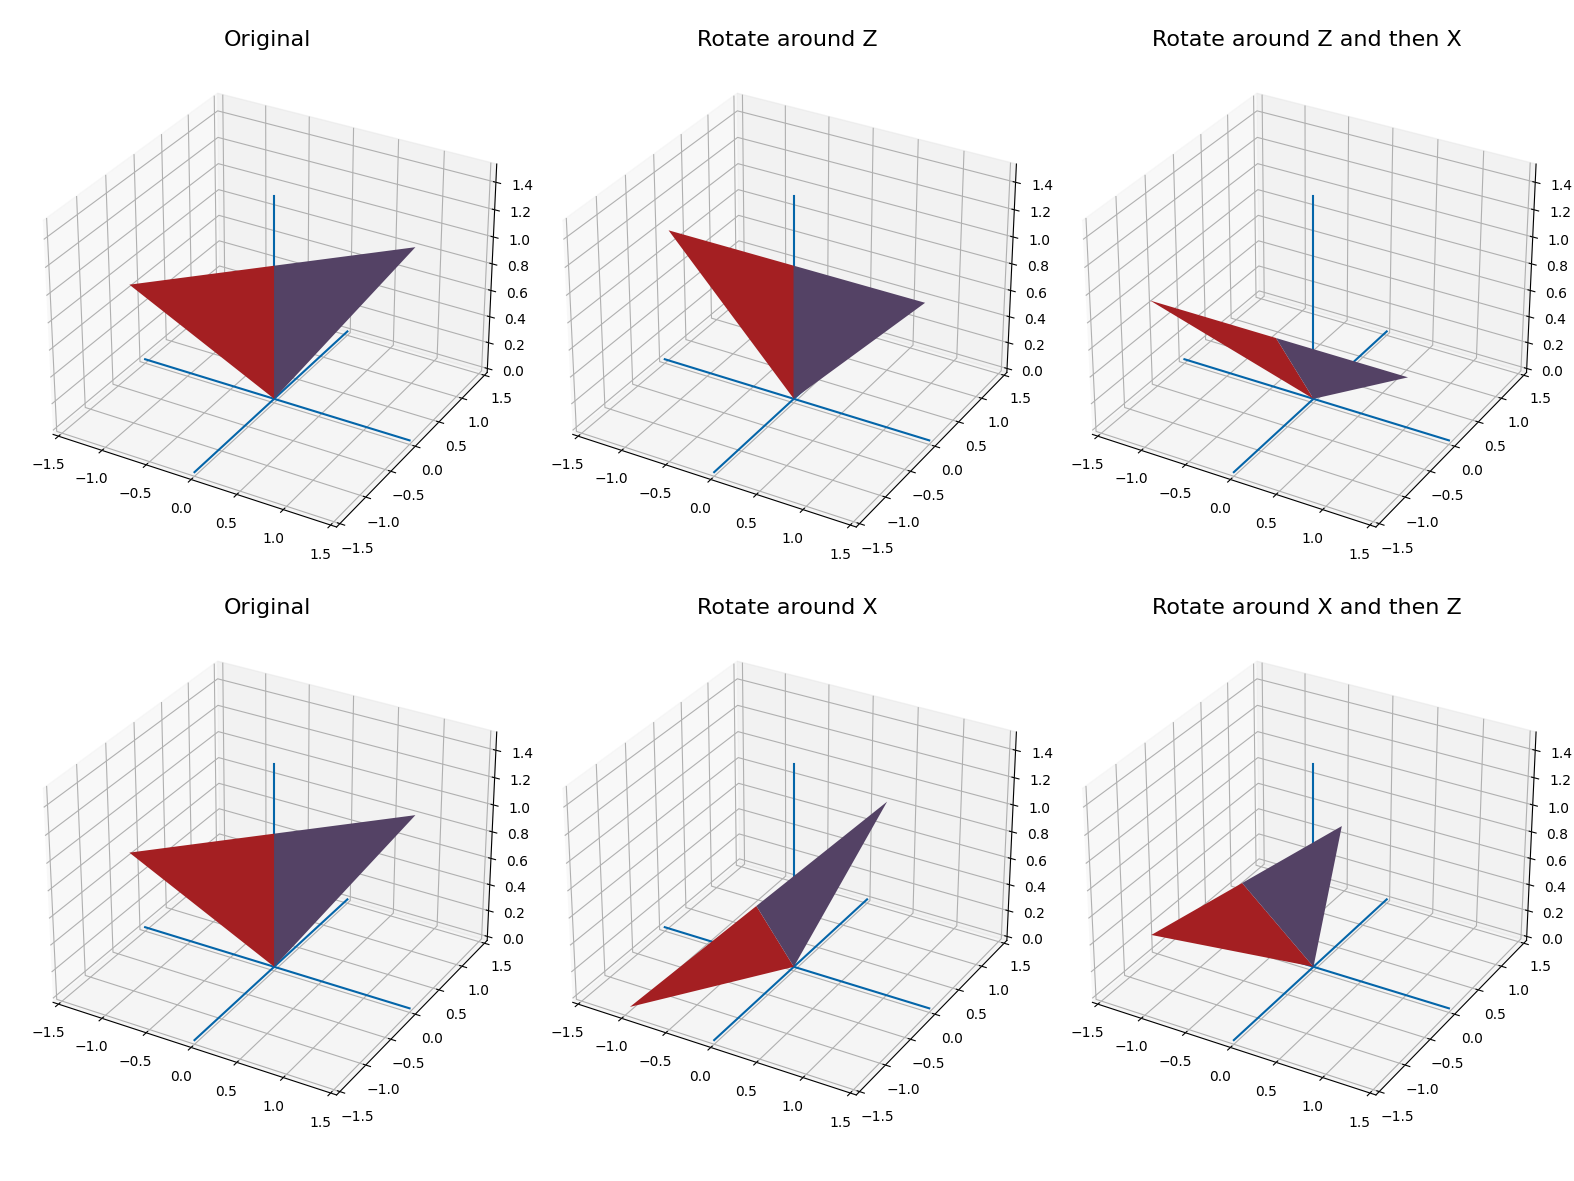
\includegraphics[width=1.0\textwidth]{images/euler_rotation.png}
    \caption{Euler rotations are dependent on the order of the individual rotations. Rotating around X and then Z results in a different outcome, than first rotating around Z and then X.}
    \label{im:EulerRotation}
\end{figure}
\subsection{Standard Vulkan Coordinate System}
In Vulkan, every vertex coordinate of a 3D rendered object gets mapped to the nearest pixel in the viewport window. This vertex mapping is done in multiple steps from "view coordinates" via "clip coordinates" towards "normalized device coordinates" to the "pixel coordinates".\\
A 3D object is a cloud of vertex coordinates described by a list three-dimensional vectors $\overrightarrow{v_{v}} = (x_{v},y_{v},z_{v})$ (the subscript $v$ denotes the "view coordinates"). These coordinates usually do not contain data regarding the whole object's scale, position, and rotation in 3D space - this information is added with matrices in the shader step.\\
Vulkan expects the output of the shader step to be in clip coordinates. Clip coordinates are four-dimensional vectors $\overrightarrow{v_{c}} = (x_{c},y_{c},z_{c},w_{c})$ (the subscript $c$ denotes the "clip coordinates") and the result of a matrix multiplication operation.\\
\begin{equation*}
    \overrightarrow{v_{c}} = A \cdot  \overrightarrow{v_{v}}
\end{equation*}
\begin{equation*}
    \begin{pmatrix}
        x_{c} \\
        y_{c} \\
        z_{c} \\
        w_{c}
    \end{pmatrix}
    =
    \begin{bmatrix}
        a_{0,0} & a_{0,1} & a_{M 0,2} & a_{0,3} \\
        a_{1,0} & a_{1,1} & a_{M 1,2} & a_{1,3} \\
        a_{2,0} & a_{2,1} & a_{M 2,2} & a_{2,3} \\
        a_{3,0} & a_{3,1} & a_{M 3,2} & a_{3,3}
    \end{bmatrix}
    \cdot
    \begin{pmatrix}
        x_{v} \\
        y_{v} \\
        z_{v} \\
        1
    \end{pmatrix}
\end{equation*}
Generally, three combined matrix multiplications describe how a 3D object is rendered – the model matrix, the view matrix, and an added projection matrix. The model matrix ($A_{Model}$) defines the scale, rotation and position of the 3D object and is a standard 4x4 matrix as explained in section \ref{sec:LinAlgRotation}.\\
The view matrix ($A_{View}$) is also is a rotation and translation matrix, but describes the position and direction of the viewport camera (or eye). Rotating the camera rotates the rendered virtual space, which indirectly moves and turns the models in the viewport. The linmath-library offers the "4x4\_look\_at" function that calculates the view matrix based on camera position, a viewing angle, and the information regarding the "upwards" direction.\\
The projection matrix ($A_{Projection}$)  is not a rotation and translation matrix besides the model and the view matrix. As its name suggests, the projection matrix reduces the vertex' 3d coordinates to the viewport plane by projecting them onto a virtual screen. By taking a field of view angle, the projection matrix allows camera distortion. The linmath-library offers the "4x4\_perspective" function that calculates the projection matrix based on a given field of view angle
Within the vertex shader, these three matrices are chained to perform the desired transformation.
\begin{equation*}
    A = A_{Projection} \cdot A_{View} \cdot A_{Model}
\end{equation*}
By division of the clip coordinate components $x_{c}$, $y_{c}$ and $z_{c}$ with $w_{c}$, Vulkan itself calculates the normalized device coordinates $\overrightarrow{v_{NDC}} = (x_{NDC}, y_{NDC}, z_{NDC})$.
\begin{equation*}
    \begin{pmatrix}
        x_{NDC} \\
        y_{NDC} \\
        z_{NDC} \\
    \end{pmatrix}
    =
    \begin{pmatrix}
        \frac{x_{c}}{w_{c}} \\
        \frac{y_{c}}{w_{c}} \\
        \frac{z_{c}}{w_{c}} \\
    \end{pmatrix}
\end{equation*}
The transformation to the pixel coordinates are also done by Vulkan without requiring any action by the developer. The only noticable detail is the alignment of the normalized device coordinates. On the viewport surface, the point $(0 / 0)$ is located in the center. Top left is $(-1 / -1)$, top right is $(1 / -1)$, bottom left is $(-1 / 1)$ and bottom right is $(1 / 1)$.

\subsection{Rotation with Quaternions}
Quaternions - also known as "Hamilton Numbers" - are the four dimensional equivalent to complex numbers. The theory of quaternions is vast, only the parts needed in this thesis are explained in this section. Analogue to complex numbers, quaternions also consist of a real part, but add three imaginary parts $\textbf{i}$, $\textbf{j}$ and $\textbf{k}$. Most often, quaternions get represented in the form $a+b\textbf{i}+c\textbf{j}+d\textbf{k}$ or a four dimensional vector $(a, b, c, d)$.\\
The relations of the different imaginary parts in a quaternion are defined as following: $\textbf{i}^{2}=\textbf{j}^{2}=\textbf{k}^{2}=\textbf{ijk}=-1$, $\textbf{ij}=\textbf{k}, \textbf{jk}=\textbf{j}, \textbf{ki}=\textbf{j}$, and  $\textbf{ji}=-\textbf{k}, \textbf{kj}=-\textbf{i}, \textbf{ik}=-\textbf{j}$. These definitions cause the quaternion multiplication (or Hamilton Product) to be non-commutative. The following equation shows how the Hamilton Product is calculated:
\begin{equation*}
    (a_{1}+b_{1}\textbf{i}+c_{1}\textbf{j}+d_{1}\textbf{k})(a_{2}+b_{2}\textbf{i}+c_{2}\textbf{j}+d_{2}\textbf{k})
    =
    \begin{pmatrix}
          & a_1a_2 &  & - b_1b_2 &  & - c_1c_2 &  & - d_1d_2             \\
        ( & a_1b_2 &  & + b_1a_2 &  & + c_1d_2 &  & - d_1c_2) \textbf{i} \\
        ( & a_1c_2 &  & - b_1d_2 &  & + c_1a_2 &  & + d_1b_2) \textbf{j} \\
        ( & a_1d_2 &  & + b_1c_2 &  & - c_1b_2 &  & + d_1a_2) \textbf{k}
    \end{pmatrix}
\end{equation*}
The neutral element of the quaternion multiplication is:
\begin{equation*}
    \begin{pmatrix}
        1           \\
        0\textbf{i} \\
        0\textbf{j} \\
        0\textbf{k}
    \end{pmatrix}
\end{equation*}
A plain three-dimensional vector is written in quaternions by only using the imaginary components.
\begin{equation*}
    \begin{pmatrix}
        x \\
        y \\
        z \\
    \end{pmatrix}
    =
    \begin{pmatrix}
        0           \\
        x\textbf{i} \\
        y\textbf{j} \\
        z\textbf{k}
    \end{pmatrix}
\end{equation*}
According to Euler's rotation theorem, providing a certain angle $\theta$ and a rotation axis $\vec{v_{r}}$, allows describing any rotation in three-dimensional space.
These values - the angle and the axis - are embedded within the rotation quaternion. In addition, the rotation quaternion is required to have the norm being equal one. Such a rotation quaternion is sometimes named a unit quaternion or a versor.
\begin{equation*}
    \vec{v}_{r} =
    \begin{pmatrix}
        x \\
        y \\
        z \\
    \end{pmatrix}
    \quad ; \quad
    \vec{v}_{r,norm} =
    \begin{pmatrix}
        \frac{x}{\lVert v_{r} \rVert} \\
        \frac{y}{\lVert v_{r} \rVert} \\
        \frac{z}{\lVert v_{r} \rVert}
    \end{pmatrix} =
    \begin{pmatrix}
        x_{norm} \\
        y_{norm} \\
        z_{norm}
    \end{pmatrix}
    \quad ; \quad
    Q_{rot}=
    \begin{pmatrix}
        \cos (\frac{\theta}{2} )                 \\
        x_{norm}\sin(\frac{\theta}{2})\textbf{i} \\
        y_{norm}\sin(\frac{\theta}{2})\textbf{j} \\
        z_{norm}\sin(\frac{\theta}{2})\textbf{k}
    \end{pmatrix}
    \quad ; \quad
    \lVert Q_{Rot} \rVert = 1
\end{equation*}
To apply this rotation quaternion $Q_{rot}$ to a vector $\vec{v}$, it needs to be conjugated and calculated from the front and from the back as shown in the following. Conjugation of a unit quaternion is done by flipping the sign in each imaginary part. Vector $\vec{u}$ is the rotated vector $\vec{v}$.
\begin{equation*}
    \vec{v} =
    \begin{pmatrix}
        a \\
        b \\
        c \\
    \end{pmatrix}
    =
    \begin{pmatrix}
        0           \\
        a\textbf{i} \\
        b\textbf{j} \\
        c\textbf{k}
    \end{pmatrix}
    \quad ; \quad
    \vec{u} = Q_{rot}\vec{v}Q_{rot}^{-1}=\begin{pmatrix}
        \cos (\frac{\theta}{2} )                 \\
        x_{norm}\sin(\frac{\theta}{2})\textbf{i} \\
        y_{norm}\sin(\frac{\theta}{2})\textbf{j} \\
        z_{norm}\sin(\frac{\theta}{2})\textbf{k}
    \end{pmatrix}
    \begin{pmatrix}
        0           \\
        a\textbf{i} \\
        b\textbf{j} \\
        c\textbf{k}
    \end{pmatrix}
    \begin{pmatrix}
        \cos (\frac{\theta}{2} )                  \\
        -x_{norm}\sin(\frac{\theta}{2})\textbf{i} \\
        -y_{norm}\sin(\frac{\theta}{2})\textbf{j} \\
        -z_{norm}\sin(\frac{\theta}{2})\textbf{k}
    \end{pmatrix}
\end{equation*}
By converting a rotation quaternion to a rotation matrix, the gap to Vulkan can be bridged. This formula only applies to true rotation quaternions, therefore the norm needs to be equal to one. 
\begin{equation*}
    Q_{Rot}=    \begin{pmatrix}
        a           \\
        b\textbf{i} \\
        c\textbf{j} \\
        d\textbf{k}
    \end{pmatrix}
    \quad ; \quad
    \lVert Q_{Rot} \rVert = 1
    \quad ; \quad
    A_{Rot}
    =
    \begin{bmatrix}
        1-2(c^{2}+d^{2}) & 2(bc-ad) & 2(bd+ac) \\
        2(bc+ad) & 1-2(b^{2}+d^{2}) & 2(cd-ab) \\
        2(bd-ac) & 2(cd+ab) & 1-2(b^{2}+c^{2})
    \end{bmatrix}
\end{equation*}
The basic quaternion operations - like the multiplication - are included in the linmath-library. The linmath-library represents a quaternion as a four-dimensional float-vector in the ordering $(b, c, d, a)$ - the real part being the last element.\\
\section{Camera Calibration}
An uncalibrated camera image often has lens distortion, warping a rectangle into a pillow or barrel shape and making areas appear closer in certain parts of the image. These distortions are named radial and tangential distortion and are induced by the camera lens.\\
According to OpenCV \cite{openCVCamCalib}, radial distiortion can be modeled as:
\begin{equation*}
x_{distorted} = x(1+k_{1}r^{2}+k_{2}r^{4}+k_{3}r^{6})\qquad
y_{distorted} = y(1+k_{1}r^{2}+k_{2}r^{4}+k_{3}r^{6})
\end{equation*}
Tangential distortion is modeled as\cite{openCVCamCalib}:
\begin{equation*}
    x_{distorted} = x+(2p_{1}xy+p_{2}(r^{2}+2x^{2}))\qquad
    y_{distorted} = y+(p_{1}(r^{2}+2y^{2})+2p_{2}xy)
\end{equation*}
In these equations, $r$ is the euclidian distance between the distorted image point and the distortion center.\cite{openCVCamCalib}\\
\begin{equation*}
    r=\sqrt{(x_{distorted}-x_{center})^{2}+(y_{distorted}-y_{center})^{2}}
\end{equation*}
Therefore, for the lens distortions, the five coefficients $k_{1}$, $k_{2}$, $k_{3}$, $p_{1}$ and $p_{2}$ are needed. In addition, the effect of the focal length $f$ and the optical center $f$ get expressed as a 3x3 matrix.\cite{openCVCamCalib}
\begin{equation*}
    A_{Camera}
    \begin{bmatrix}
        f_{x} & 0 & c_{x} \\
        0 & f_{y} & c_{y} \\
        0 & 0 & 1
    \end{bmatrix}
\end{equation*}
OpenCV itself provides a script which estimates these values based on multiple photographs of chess boards. Applying these corrections leads to a smaller image as parts near the border get cut off.
\begin{figure}[H]
    \centering
    \begin{minipage}[b]{0.45\textwidth}
      
\includegraphics[scale=0.70]{images/camcalib_source.jpg}
      \caption{Before correction}
      \label{fig:heightmapdots} 
    \end{minipage} % Hier darf keine Leerzeile zwischen den beiden Minipages liegen!
    \begin{minipage}[b]{0.45\textwidth}
      
\includegraphics[scale=0.70]{images/camcalib_result.png} 
      \caption{After correction}
      \label{fig:bothobjects} 
    \end{minipage}
    \caption{Camera correction demonstrated at the grayscale image of the ToF camera.}
    \label{fig.videodisplay}
  \end{figure}
 
%!TEX root = ../doc.tex
\chapter{Implementation}
\label{sec:Implementation}
This chapter describes the implementation and the connections of the individual components of the augmented reality system. There are two main tasks, the system needs to perform: A three dimensional estimation of the surrounding and the precise measurement of motion of the camera head.
\section{Hardware}
\label{sec:Hardware}
The following section describes the evaluation and setup of the hardware used for the camera head and the processing system. 
\subsection{Evaluation of ToF Camera}
\label{sec:CamEvaluation}
Having no prior experience with time-of-flight (ToF) cameras, a suitable device had to be evaluated first. Cost and availability have been the main factors in the evaluation, with it being directly CSI-2 connected being a big plus.\\
Internet research has shown a handful of different sensors powering multiple products of other manufacturers in varying price ranges. \\
\\
\textbf{Sony DepthSense IMX556PLR}\\
The Sony IMX556PLR ToF Sensor offers a resolution of 640 x 480 pixels at 30 frames per second and is used by Basler, Lucid Vision Labs, and DephtEye, primarily for Gigabit Ethernet cameras. The IMX556PLR seems to be the most capable ToF sensor freely available in off-the-shelf products at the time.  \\
The technically most compelling product for this thesis would have been the Helios Flex by Lucid Vision Labs, which directly connects via CSI-2 and is sold specifically for use on an Nvidia Jetson TX2 Developer Kit. It features a maximum range of 6 meters for depth measurement and accuracy of ±10mm. Although with 749 US Dollars, the Helios Flex is relatively expensive and unsuitable for the thesis because of an unknown lead time.\\
\\
\textbf{Infineon REAL3 IRS1125}\\
The Infineon IRS1125 ToF Sensor is available in a USB-based development kit by pmdtec – an integrator for ToF technology into smartphones – and on the affordable PiEye Nimbus 3D camera, which is sold as a Raspberry Pi accessory.  \\
The sensor features a resolution of 352x288 pixels at 30 frames per second in the variant IRS1125A. The variant IRS1125C – used by pmdtec – allows 60 frames per second. The pmdtec development kit is tuned for measuring up to 6 meters, while the PiEye camera is limited to 5 meters.\\
While both camera systems are readily available to be shipped, the pmdtec pico monstar costs about 1500 US Dollars; in contrast, the PiEye Nimbus costs only 230 Euros. The PiEye company advertises its camera with open source software to embed it into the Raspberry Pi ecosystem. However, further investigation has shown that the middleware – the library managing the camera’s settings and connecting to the video4linux2 framework – is still under NDA with Infineon. \\
With a lightweight TCP/IP protocol, the module is suitable with a Raspberry Pi, acting as a Gigabit Ethernet camera. The PiEye Nimbus is the module of choice for this thesis – the availability, the price, and the specifications are all reasonable. The options to reverse engineer the middleware or sign an individual NDA with Infineon have been kept open initially but were not necessary as the Gigabit Ethernet implementation worked well enough.\\
\\
\textbf{Other image sensors}\\
During the internet research, the Texas Instruments OPT8241 has shown up. TI declared the chip obsolete – the chip itself was still available, but the development kit was sold out. With 320 times 240 pixels and an advertised range of 4 meters, the OPT8241 is inferior to the chosen PiEye Nimbus. In addition, the Terabee 3Dcam features a custom sensor with a resolution of 80x60 pixels and 4 meters range. It is attached by USB 2.0 and costs 250 Euros. Due to the low resolution, the Terabee 3Dcam is also inferior to the PiEye Nimbus. 


\subsection{Camera Head}
\label{sec:camHead}
The camera head contains the PiEye Nimbus ToF camera, mounted on a Raspberry Pi 4B, a Bosch BMI160 IMU, attached to a USB to I²C bridge, and a standard Raspberry Pi camera v2.1 which is connected to the processing system via an FPDLink module.\\
All is held together by a plywood structure glued onto a tripod-baseplate, shown in figure \ref{fig:cameraHead}.
\begin{figure}[H]
    \centering
    \begin{minipage}[b]{0.45\textwidth}
      
\includegraphics[scale=0.40]{images/todo.png}
      \caption{Frontside}
      \label{fig:cameraHeadfront} 
    \end{minipage} % Hier darf keine Leerzeile zwischen den beiden Minipages liegen!
    \begin{minipage}[b]{0.45\textwidth}
      
\includegraphics[scale=0.40]{images/todo.png} 
      \caption{Backside}
      \label{fig:cameraHeadback} 
    \end{minipage}
    \caption{The camera head consisting of the ToF camera, the IMU and the Raspberry Pi camera}
    \label{fig:cameraHead}
  \end{figure}
The IMU could have been attached directly to the Raspberry Pi, but at the time of the implementation, the decision on how to connect the ToF camera was not taken yet. Therefore, it was not certain that a Raspberry Pi would be mounted at the camera head.
Four individual cables connect to the different components on the camera head: A USB-C power cable and an RJ45 Ethernet cable for the Raspberry Pi, a USB 2.0 cable for the USB to I²C bridge, and an FPDLink coaxial cable for the Raspberry Pi Camera.


\subsection{Processing System}
\label{sec:procSystem}
An Nvidia Jetson Xavier AGX in the 8GB version carries out the processing, rendering, and data acquisition. An Anyvision baseboard - shown in image \ref{fig:anyvision} - carries the Nvidia Jetson module and allows the direct attachment of the used data cables.
\begin{figure}[H]
    \centering
    
\includegraphics[width=1.0\textwidth]{images/todo.png}
    \caption{The Nvidia Jetson Xavier AGX on the Anyvision Baseboard.}
    \label{fig:anyvision}
\end{figure}
A TCP/IP server application on the Raspberry Pi powering the PiEye ToF camera, to which the processing system connects, serves the necessary ToF camera data in a frame-based protocol. The USB to I²C bridge gets loaded as a standard I²C device by the Linux on the processing system. The IMU is then directly configured and polled by the userspace software on the processing system without an additional driver. The Raspberry Pi camera is attached via FPDLink and integrated as a video4linux2 device. The capturing is done with FFMPEG and the debayering in CUDA.
\section{Video inputs}
\label{sec:videoInputs}
The system utilizes two cameras, a Raspberry Pi Camera v2 and a PiEye ToF camera that doubles as an infrared camera. The Sony IMX 219 based Raspberry Pi Camera v2 features a color image with an 8 megapixel resolution for single images, 1080p with 30 frames per second, 720p with 60 frames per second or 480p with 90 frames per second.\cite{raspiCamSpec} The Raspberry Pi Camera v2 is a Mipi CSI2 attached camera module whichs cable length got extended by an FPDLink serializer and deserializer.\\
The PiEye ToF camera is based on the Infineon REAL3 IRS1125A sensor which has a resolution of 352 x 288 pixels\cite{piEyeShop}. The ToF Camera is paired with infrared LED flashes to measure the time of flight of the light emitted and has an intended measurement range from 10 centimeters up to five meters. The entire ToF software stack runs on a Raspberry Pi that sends its video data via Ethernet to the augmented reality system.\\

\subsection{ToF Camera calibration}
\label{sec:ToFCalibration}
On the ToF Camera, two parts need to be calibrated: The optics, as described in section \ref{sec:FundCamCalibration}, and the distance measurement. The ToF camera has a barrel type distortion that is corrected by the camera calibration algorithm implemented in OpenCV\cite{openCVCamCalib} and shown in image \ref{fig.camCalib}. As the process of lens correction cuts off parts of the image, the image size gets lowered to 265 x 205 pixels.\\
For the distance measurement, first the radial distances need to be flattened as described in section \ref{sec:RadialCorrection}. As the angle $\alpha$ is not known for each pixel, a reference measurement provides the necessary information. To reduce noise, 19 images of the same flat wall has been taken, smoothed by a gaussian and averaged onto one reference image $I_{Ref}$. The wireframe image in figure \ref{im:ToFRaw} shows the curvature of the reference image. The rounding at the edges is an arfifact of the gaussian smoothing.\\
\begin{figure}[H]
    \centering
    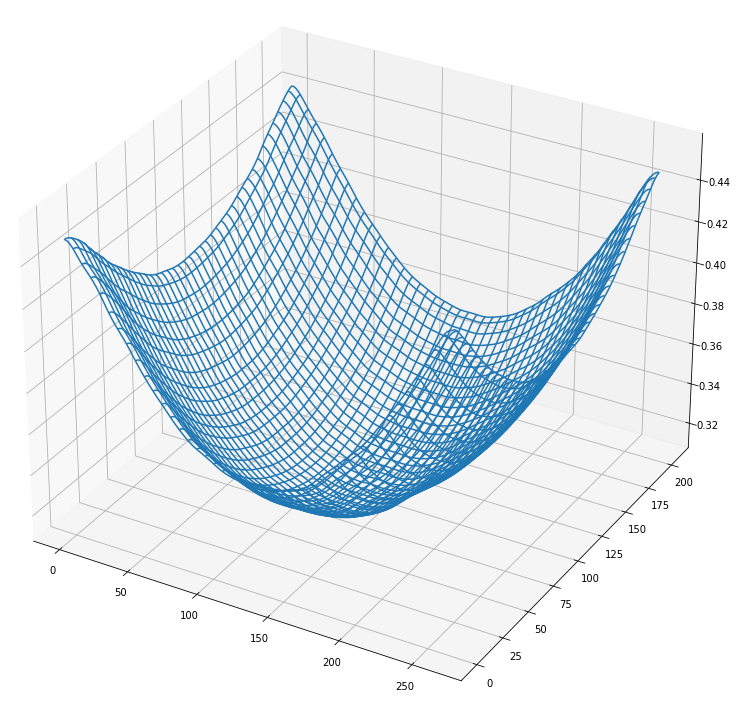
\includegraphics[width=0.4\textwidth]{images/raw_tof_radial.png}
    \caption{Wireframe rendering of the reference image $I_{Ref}$ provided by the ToF camera}
    \label{im:ToFRaw}
\end{figure}
Dividing the minimum value of this reference image $I_{Ref}$ with every pixel value generates a map of $\cos \alpha$ named $I_{cos}$.
\begin{equation*}
    I_{cos} = \frac{\min (I_{Ref}) }{I_{Ref}} 
\end{equation*}
Pixel by pixel multiplication of any other image $I_{Any}$ with $I_{cos}$ will correct the influence of the radial measurement as shown in image \ref{im:ToFCorrected}. 
\begin{equation*}
    I_{Corr} = I_{cos}\cdot I_{Any}
\end{equation*}
\begin{figure}[H]
    \centering
    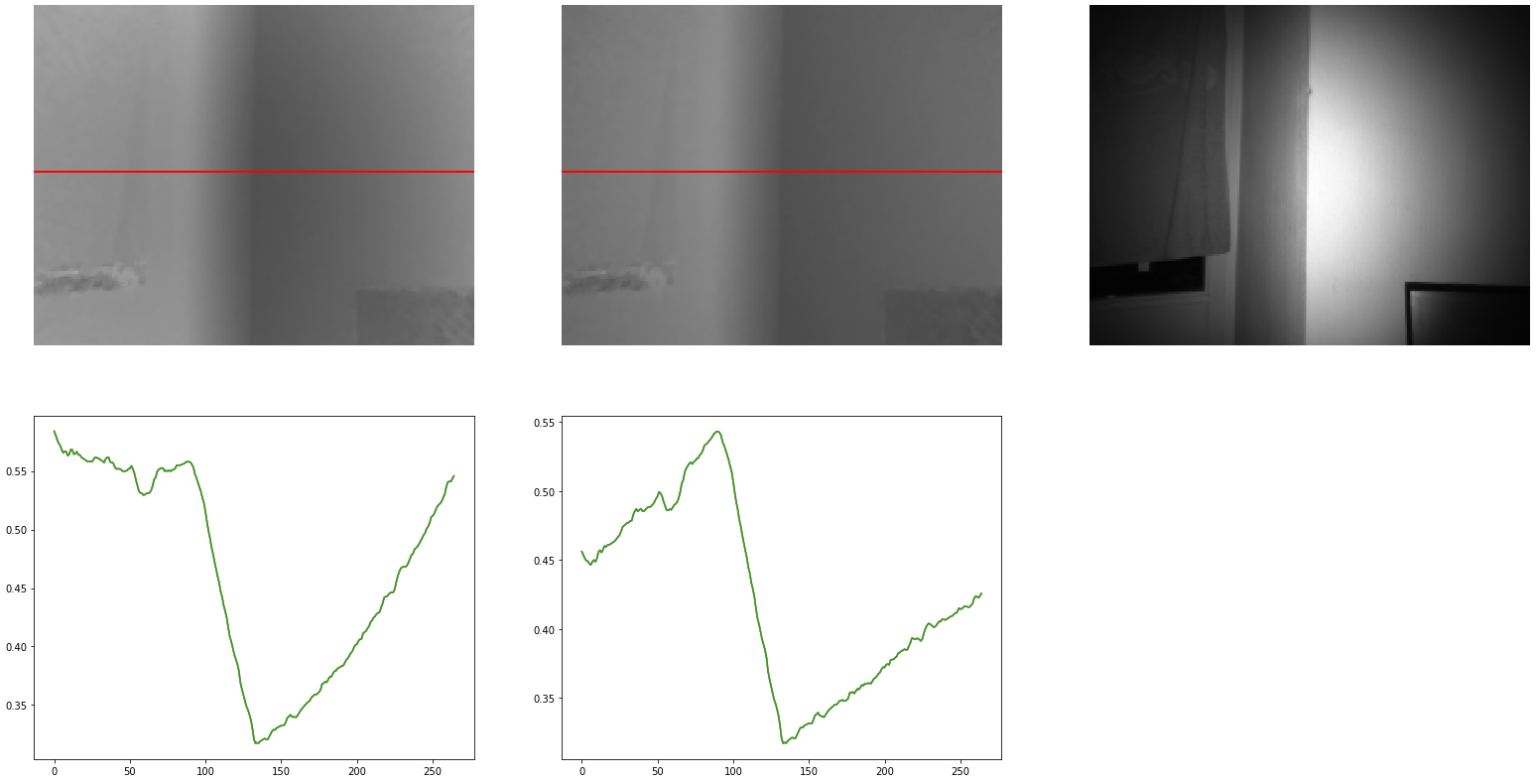
\includegraphics[width=1.0\textwidth]{images/flattened_tof_example.png}
    \caption{Left, the uncorrected ToF image $I_{Any}$, in the middle the corrected image $I_{Corr}$ and on the right, the infrared grayscale image of the scene. To make the effect more apparent, the brightness accross the red lines have been plotted.}
    \label{im:ToFCorrected}
\end{figure}
To apply this calibration in CUDA, a file has been generated which holds the $I_{Cos}$ values for each pixel. The application reads the file at initialization and keeps it stored in a Cuda allocated memory area. 


TODO: Distance measurement calibration!
\subsection{Raspberry Pi Camera calibration}
\label{sec:RBPiCalibration}
TODO: Cam calibration
\section{Gyroscope and Accelerometer Calibration}
\label{sec:GyroCal}
The used inertial movement unit (IMU) is a Bosch BMI160, that is sold soldered on a PCB by DFRobot.\\
As the gyroscope and accelerometer output incremental movement, the values need to be integrated over time. Accurate data is crucial for finding the direction of gravity or detecting movement - especially because of positional information being the result of derivating the acceleration twice.\\
The range of the acclerometer is variable and has been set to ±8 G, it has an output resolution of 16 bit and an output data rate of 200 Hz.
The accelerometer has been calibrated in 24 orientations to even out angle errors inside the IMU, on the PCB and of the calibration table, as shown im image \ref{im:IMU_cal}. For each orientation, 100 raw measurements have been averaged to even out noise. 
\begin{figure}[H]
    \centering
    
\includegraphics[width=1.0\textwidth]{images/todo.png}
    \caption{The 24 orientations used for calibration - four directions for each of the six sides.}
    \label{im:IMU_cal}
\end{figure}
The largest error has been 38 mG, that lies within the sensor's specification of ±40 mG\cite{BMI160}. In addition, the gain for the accelerometer has been corrected based on gravity. A maximum error of 1.8\% has been measured and corrected, which also lies in the sensor's specification of ±0.5\% full scale\cite{BMI160}.\\
For the gyroscope, the range is set to ±2000 degrees per second with an output data rate of 200 Hz. The gyroscope has been calibrated only for zero offset, whose maximum error was 0.2 degrees per second which lies well in the specified ±3 degrees per second\cite{BMI160}. A gain correction was not made, because of not having the required equipment to do so.\\
\section{Position and Orientation Estimation}
\label{sec:PositionEstimate}
The position estimation of the camera head is crucial for the augmented reality platform. The following section describes the implementation of the different systems involved in sensing motion.\\
While the measurement using the IMU is standard implementation via I²C communication, the implementation of the ToF-Camera based measurement is more complex and got split into multiple subsections. 
\subsection{Spatial coordinates and device coordinates}
\label{sec:ABC_XYZ_coords}
As the rotation of the camera head changes the coordinates of the measurement in respect to real-world coordinates, a convention helps carry out the calculations. For the sensors on the camera head, the coordinates are named $a$, $b$, and $c$, while the spatial coordinates are named $x$, $y$, and $z$.
The coordinates can be transformed by the following formula, knowing the current orientation quaternion $Q_{rot}$.   
\begin{equation*}
    Q_{rot}
    =
    \begin{pmatrix}
        r           \\
        u\textbf{j} \\
        v\textbf{j} \\
        w\textbf{k}
    \end{pmatrix}
    \quad ; \quad
    \begin{pmatrix}
        0           \\
        x\textbf{i} \\
        y\textbf{j} \\
        z\textbf{k}
    \end{pmatrix}
    =
    \begin{pmatrix}
        r           \\
        u\textbf{i} \\
        v\textbf{j} \\
        w\textbf{k}
    \end{pmatrix}
    \begin{pmatrix}
        0           \\
        a\textbf{i} \\
        b\textbf{j} \\
        c\textbf{k}
    \end{pmatrix}
    \begin{pmatrix}
        r           \\
        -u\textbf{i} \\
        -v\textbf{j} \\
        -w\textbf{k}
    \end{pmatrix}
\end{equation*}
Section \ref{sec:RotationQuaternion} describes how to carry out the mathematics of this quaternion multiplication. 
\subsection{Gyroscope and Accelerometer}
\label{sec:GyroPosition}
The 6-axis IMU Bosch BMI160 provides gyroscope and accelerometer measurements via an I²C connection, extended by a Silicon Labs CP2112 USB-to-I²C bridge. The IMU generates measurements regarding acceleration in the directions $a$, $b$, and $c$, and measurements regarding rotation speed around these axes.\\
The IMU shows a hysteresis that lies within the specification of the datasheet; therefore, a simple offset correction does not yield the best results. A moving average – that gets updated whenever no motion of the camera head is detected – helps deal with the hysteresis by subtraction from the measurement value.
\subsection{ToF Camera: SIFT feature extraction}
\label{sec:ToFPosition_SIFT}
The PiEye Nimbus ToF camera generates three different image channels for each picture taken: The depth map, the confidence, and the greyscale infrared image. By correcting the lens distortion as described in chapter \ref{sec:FundCamCalibration}, straight lines in the real world get projected as straight lines on the images. By further correcting the characteristic of the ToF camera to measure radial distances, as described in section \ref{sec:RadialCorrection}, flat surfaces in the real world are also flat on the depth map. The implementations of both corrections are explained in section \ref{sec:ToFCalibration}. \\
The points of the point clouds need to be matched to estimate rotation and translation between two consecutive ToF images. The CudaSift library\cite{cudaSiftRepo}\cite{CudaSiftPublication} extracts SIFT\cite{siftpaper} features on each greyscale infrared image the ToF camera sends $k$, which are then brute-force matched with the features of the prior image $k-1$, as visualized in image \ref{im:SiftExtraction}. SIFT features were chosen because of the author's prior experience, and it is a well-known feature extraction algorithm whose patent expired.\cite{siftpatent}
\begin{figure}[H]
    \centering
    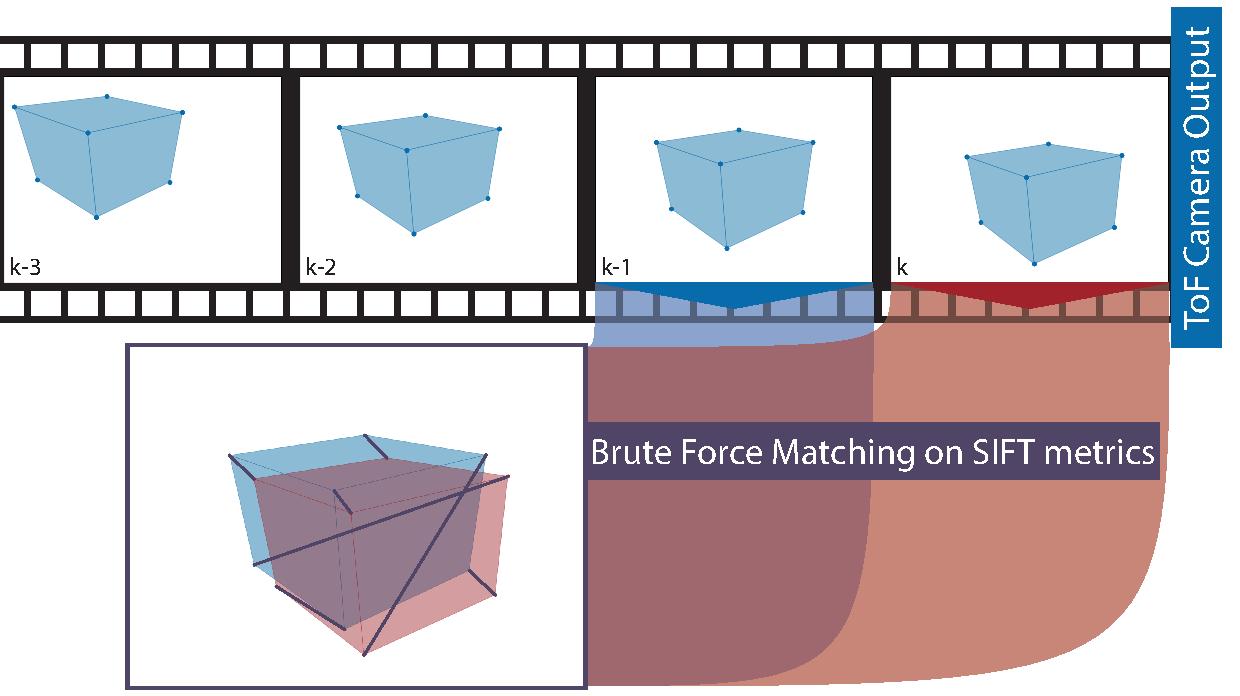
\includegraphics[width=1.0\textwidth]{images/feature_matching_bruteforce.pdf}
    \caption{First step of ToF motion estimation: Extract SIFT features and brute-force match with prior image. Note that the brute-force matcher also generates false matches.}
    \label{im:SiftExtraction}
\end{figure}
Each feature coordinate on the picture gets mapped to the 3D space to generate the point cloud. The lens projects objects within the space of a pyramid onto the sensor, which leads to the following coordinate mapping. The coordinate transformation is visualized in image \ref{im:SiftCoordTransform}. Please note the coordinate convention described in section \ref{sec:ABC_XYZ_coords}. $a$, $b$ and $c$ being the 3D coordinates, $u$ and $v$ being the coordinates on the image and $d$ being the value of the ToF depth image on position $(u,v)$. $f$ denotes a virtual focal length, merging the camera's field of view (viewing angle $\alpha$) and the image resolution in one number.
\begin{equation*}
    a = d \qquad b = \frac{v}{f}\cdot x \qquad c = \frac{u}{f}\cdot x \qquad f=\frac{\tfrac{u_{max}}{2}}{tan(\tfrac{\alpha}{2})}
\end{equation*}
The PiEye Nimbus ToF camera has an advertised viewing angle of $1.152rad$ horizontally and $0.942rad$ vertically. Combined with an image resolution of $352 x 288px$, the formula for $f$ outputs $271$ for the horizontal and $282$ for the vertical case. The chosen value is: $f = 280$.
\begin{figure}[H]
    \centering
    
\includegraphics[width=1.0\textwidth]{images/todo.png}
    \caption{Second step of ToF motion estimation: Map features into 3D space}
    \label{im:SiftCoordTransform}
\end{figure}
\subsection{ToF Camera: Find rotation and translation}
\label{sec:ToFPosition_SVD}
Calculating the rotation and translation of one point cloud $P_{k-1}$ to another point cloud $P_{k}$ is possible with at least three correctly matched point pairs. Following the recipe from a note from the ETH Zurich, also containing the proof, the three points must be centered. The method described in the ETH note also adds the possibility to add weights to individual data points. Upper case $P$ denotes a point cloud, lower case $p$ denotes a single point in that cloud. The number of matched point pairs in the following formulae is $n$, in the example $n = 3$, $i$ is the index of the single point in the point cloud and $k$ is the image frame number from which the point cloud got extracted.
The centroids for both point groups are:
\begin{equation*}
    \vec{c}_{k}=\frac{\sum_{i=1}^n \vec{p}_{i,k}}{n} \qquad 
    \vec{c}_{k-1}=\frac{\sum_{i=1}^n \vec{p}_{i,k-1}}{n}
\end{equation*}
For example visualized in image \ref{im:SVD_step_by_step} and with the following calculation:

\begin{equation*}
    \vec{c}_{k}=
    \begin{pmatrix}
        NUM \\
        NUM \\
        NUM
    \end{pmatrix}
    =\frac{1}{3}\cdot\left(
    \begin{pmatrix}
        NUM \\
        NUM \\
        NUM
    \end{pmatrix}
    +
    \begin{pmatrix}
        NUM \\
        NUM \\
        NUM
    \end{pmatrix}
    +
    \begin{pmatrix}
        NUM \\
        NUM \\
        NUM
    \end{pmatrix}
    \right)
\end{equation*}
\begin{equation*}
    \vec{c}_{k-1}=
    \begin{pmatrix}
        NUM \\
        NUM \\
        NUM
    \end{pmatrix}
    =\frac{1}{3}\cdot\left(
    \begin{pmatrix}
        NUM \\
        NUM \\
        NUM
    \end{pmatrix}
    +
    \begin{pmatrix}
        NUM \\
        NUM \\
        NUM
    \end{pmatrix}
    +
    \begin{pmatrix}
        NUM \\
        NUM \\
        NUM
    \end{pmatrix}
    \right)
\end{equation*}
\begin{figure}[H]
    \centering
    
\includegraphics[width=1.0\textwidth]{images/todo.png}
    \caption{Rotation and Translation step by step.}
    \label{im:SVD_step_by_step}
\end{figure}
Subtraction of the centroid vectors from the individual points in the respective point cloud $P$ generates the centered point clouds $Q$. In an ideal case, a rotation matrix alone can transform one centered point cloud into the other. 
\begin{equation*}
    \vec{q}_{i,k}=\vec{p}_{i,k}+\vec{c}_{k} \qquad 
    \vec{q}_{i,k-1}=\vec{p}_{i,k-1}+\vec{c}_{k-1} 
\end{equation*}
In the example, the results are:
\begin{equation*}
    \vec{q}_{1,k}=
    \begin{pmatrix}
        NUM \\
        NUM \\
        NUM
    \end{pmatrix}
    \qquad 
    \vec{q}_{2,k}=
    \begin{pmatrix}
        NUM \\
        NUM \\
        NUM
    \end{pmatrix}
    \qquad     \vec{q}_{3,k}=
    \begin{pmatrix}
        NUM \\
        NUM \\
        NUM
    \end{pmatrix}
\end{equation*}
\begin{equation*}
    \vec{q}_{1,k-1}=
    \begin{pmatrix}
        NUM \\
        NUM \\
        NUM
    \end{pmatrix}
    \qquad 
    \vec{q}_{2,k-1}=
    \begin{pmatrix}
        NUM \\
        NUM \\
        NUM
    \end{pmatrix}
    \qquad     \vec{q}_{3,k-1}=
    \begin{pmatrix}
        NUM \\
        NUM \\
        NUM
    \end{pmatrix}
\end{equation*}
A matrix-multiplication of the point groups $Q_{k}$ and $Q_{k-1}$ generates the $3\times3$ covariance matrix $S$ as shown in the following formula. The point groups are packed in matrix form, in the three point example, the point group matrices are of dimension $3\times3$. When using $n$ points, the point group matrices are of dimension $n\times3$, whose covariance matrix remains of dimension $3\times3$.
\begin{equation*}
    S= Q_{k}Q_{k-1}^{T}
\end{equation*}
In the example:
\begin{equation*}
    Q_{k}=
    \begin{bmatrix}
        NUM & NUM & NUM \\
        NUM & NUM & NUM \\
        NUM & NUM & NUM
    \end{bmatrix} \quad
    Q_{k-1}=
    \begin{bmatrix}
        NUM & NUM & NUM \\
        NUM & NUM & NUM \\
        NUM & NUM & NUM
    \end{bmatrix}
\end{equation*}
\begin{equation*}
    S= 
    \begin{bmatrix}
        NUM & NUM & NUM \\
        NUM & NUM & NUM \\
        NUM & NUM & NUM
    \end{bmatrix}
\end{equation*}
The singular value decomposition (SVD), briefly explained in section \ref{sec:SVD}, splits the covariance matrix $S$ into three separate $3\times3$ matrices $U$, $\Sigma$, and $V$. As the SVD in this use case is always applied to matrices of dimension $3\times3$, the optimized variant\cite{Gao:2018:GPU_MPM} from GitHub\cite{Github_SVD_CUDA} can be utilized.
\begin{equation*}
    S= U\Sigma V^{T}
\end{equation*}
In the example:
\begin{equation*}
    U=
    \begin{bmatrix}
        NUM & NUM & NUM \\
        NUM & NUM & NUM \\
        NUM & NUM & NUM
    \end{bmatrix} \quad
    \Sigma=
    \begin{bmatrix}
        NUM & NUM & NUM \\
        NUM & NUM & NUM \\
        NUM & NUM & NUM
    \end{bmatrix} \quad
    V=
    \begin{bmatrix}
        NUM & NUM & NUM \\
        NUM & NUM & NUM \\
        NUM & NUM & NUM
    \end{bmatrix}
\end{equation*}
The wanted rotation matrix then follows by calculating:
\begin{equation*}
    R=V
    \begin{bmatrix}
        1 & 0 & 0 \\
        0 & 1 & 0 \\
        0 & 0 & det(VU^{T})
    \end{bmatrix}U^{T} \quad
\end{equation*}
Without the correction of the calculation, using the term $det(VU^{T})$ in the intermediate matrix, the SVD could generate a reflection instead of a rotation. This is numerically sound, but would not reflect the real world scenario. The determinant $det(VU^{T})$ equals -1 in the case of a reflection, which can be used to flip the signs of the 3rd column of the rotation matrix. If the SVD directly generates a rotation, $det(VU^{T})$ equals to 1, which transforms the intermediate matrix into the identity.\\
In the example the resulting rotation matrix $R$ equals:
\begin{equation*}
    R=
    \begin{bmatrix}
        NUM & NUM & NUM \\
        NUM & NUM & NUM \\
        NUM & NUM & NUM
    \end{bmatrix} \quad
\end{equation*}
The wanted translation is computed by applying the rotation to the centroid vectors. 
\begin{equation*}
    \vec{t} = \vec{c}_{k}-R\cdot\vec{c}_{k-1}
\end{equation*}
In the example:
\begin{equation*}
    \vec{t} = 
    \begin{pmatrix}
        NUM \\
        NUM \\
        NUM
    \end{pmatrix}
\end{equation*}


\subsection{ToF Camera: 3D ransac}
\label{sec:ToFPosition_RANSAC}
The motion estimation of the ToF camera relies on having good matches, which is not the case with the brute-force matcher, as the authors of the CudaSift library claim to have less than 50\% accuracy on its brute-force matcher.\cite{cudaSiftRepo} Low matching accuracy is a known problem in other fields of image processing - like panorama stitching - and is there often solved with an algorithm named RANSAC (random sample consensus).\\
These applications of the RANSAC algorithm work on two-dimensional images and are not suitable for three-dimensional point clouds; therefore, the RANSAC algorithm got extended.\\
The first step of the three-dimensional RANSAC is finding a proper rotation and translation from the brute-force matches. To find these transformations, each matched feature pair gets two other feature pairs randomly assigned. Using the method described in section XY, the corresponding rotations and translations are calculated on these groups of three feature pairs.\\
Each group's calculated rotation matrices and translation vectors get checked against all the other matched feature pairs. The data point from the previous image of the feature pair gets moved by the matrix-vector-pair and compared to the data point of the current picture. If the distance of the two points is underneath a threshold, the feature pair is counted for the matrix-vector-pair. On these feature pairs, the average distance from the calculated points to the matched points is measured. The matrix-vector-pair that generates the smallest average distance is likely suitable for further processing.\\
Ignoring the SIFT metrics that lead to the brute force matching, all the features get matched anew based on the position alone, using the rotation and translation estimated before. The matrix-vector pair transforms every data point from the previous image. The distance between the transformed point and the closest data point of the current picture determines the new match. If the proximity is below a threshold, the match is accepted.\\
Finally, the optimal rotation matrix and translation vector are calculated using the method described in section XY, this time not with only three points but all accepted matches. With more than three points, the calculated rotation and translation is not the exact result, but the result that yields the least square error.\cite{SVD_ETH}\\
The whole methodology relies on finding the correct rotation and translation from randomized 






\subsection{Sensor Fusion with Kalman Filter}
\label{sec:SensorFusion}
TODO: Position estimate slow
\section{Video display}
\label{sec:VideoDisplay}
TODO: Vulkan Output 
%!TEX root = ../doc.tex
\chapter{Testing and Results}
\label{sec:Results}
The following chapter describes the calibration, testing and the results of the system components. 
\section{Performance}
\label{sec:performance}
Even though, no performance optimization was done, the frame rates got measured. Activating the FFMPEG capture for the Raspberry Pi Camera causes a performance hit, that not only affects other CUDA processes, but also Vulkan. The framerates have thus been measured with and without activated FFMPEG capture. 
\begin{table}[H] \centering
	\begin{tabular}{|p{3.3cm}|p{2.5cm}|p{2.5cm}|p{2.5cm}|p{2.5cm}|} \hline
		\rowcolor{gray} Measurement & ToF Camera & IMU & Vulkan & RPi Camera \\
		\hline
		With RPi Camera & 7.85 fps & 202.01 Hz & 42.08 fps & 42.50 fps\\
		\hline
		Without RPi Camera & 11.19 fps & 200.66 Hz & 107.41 fps & - \\
		\hline
	\end{tabular}
	\caption{Average Framerates with and without activated FFMPEG Raspberry Pi Camera capture}
	\label{tab:performance}
 \end{table}
 The thread with the ToF Camera involves the whole SIFT feature extraction, RANSAC matching and the evaluation of the rigid motion. The IMU thread only polls an open I2C connection and sums up values.Because of this performance hit, the following measurements got recorded without activated FFMPEG RPi Camera. Instead of the RaspberryPi Camera, the ToF camera's debug image got drawn onto the viewfinder.
\section{ToF Camera}
The time-of-flight camera is the main part of this thesis, allowing a three-dimensional scene reconstruction. This section describes the measurements and the results of the motion estimation using this camera at every involved step.
\subsection{Setup}
As described in Section \ref{sec:camHead}, the ToF camera sends its data by ethernet, using a lightweight TCP protocol. The software controlling the setup of the ToF camera runs on the Raspberry Pi and is the proprietary part of the ToF software stack. The software allows a basic configuration in two main modes: automatic and manual control. The software supports HDR functionality in both automatic and manual control, which significantly enhances the dynamic range on the infrared black-and-white image.\\ 
The ToF camera uses an infrared flash, which is not brightness-controlled. Setting the camera to a fixed exposure time would lead to overexposure on close objects. The automatic mode lets the user select a maximum amplitude of the image, to which the exposure time is set. As the CudaSift library, which extracts the SIFT features from the ToF camera, only supports the 8-bit resolution, the maximum amplitude was set to 255. Higher values lead to a longer exposure time and let the frame rate drop. Not needing any amplitude scaling while keeping a high frame rate is favorable.\\
The coordinate system is not corrected for $x$, $y$ and $z$ yet, as the ToF camera itself does not know its rotation in the field of gravity. Therefore, the axis for the ToF camera calculations are kept in the $a$, $b$ and $c$ system. Details are explained in Section \ref{sec:ABC_XYZ_coords}.
\subsection{Distance measurement}
\label{sec:results_distance_meas}
Every pixel of a ToF camera sensor combined with the wide-area infrared flash acts like a laser rangefinder. A single pixel of the sensor targeting a brown cardboard surface positioned at various distances allows measuring this distance with a folding meter and a comparison with the sensor pixel value. Fitting a line to the measured data points gives the linear relation from the distance
\begin{equation*}
    d [m] = 0.000227 * val +0.247532
\end{equation*}
to the camera value $val$.
\begin{figure}[H]
  \centering
  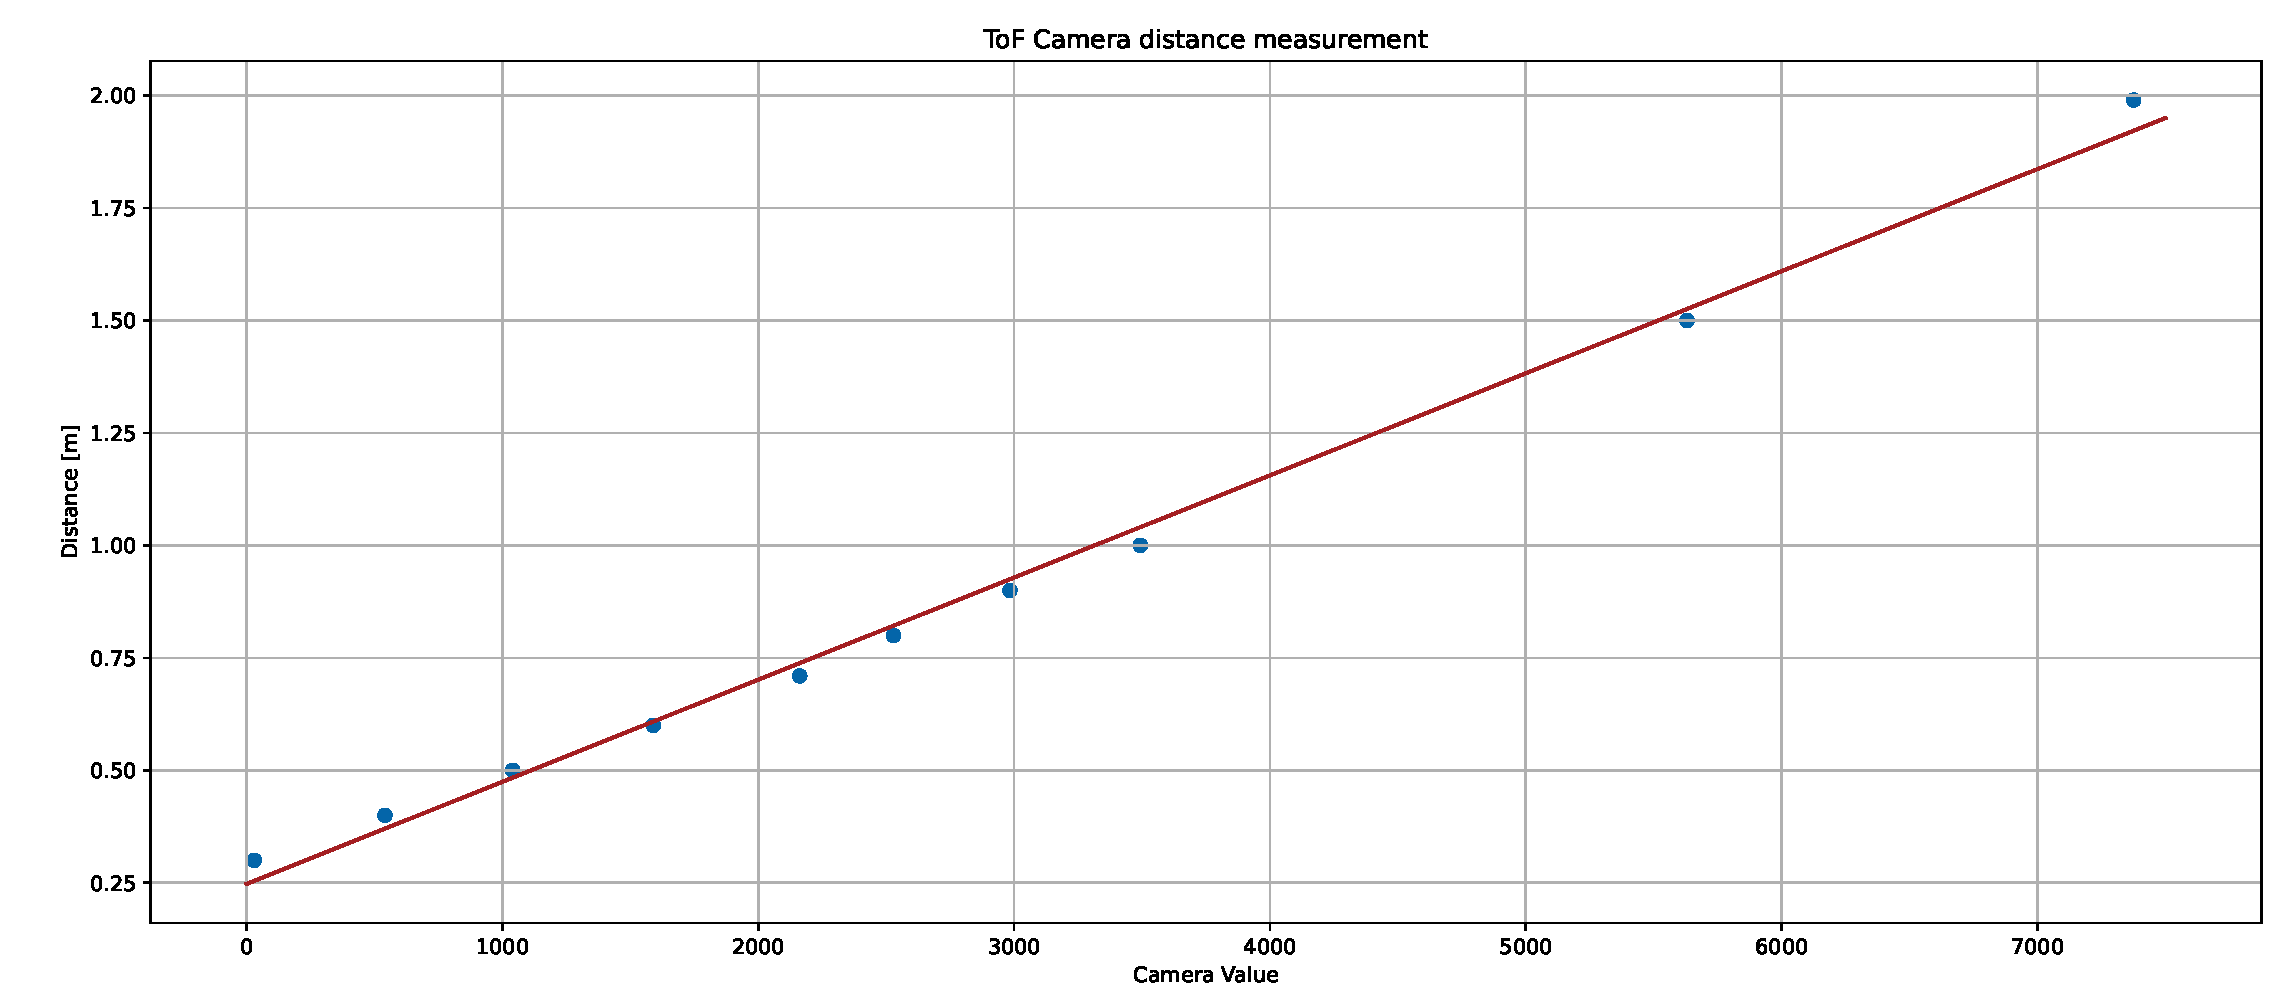
\includegraphics[width=1.0\textwidth]{images/camera_distance_measurement.eps}
  \caption{Sensor values measured against a folding meter. The red curve shows a linear fit of the data points.}
  \label{im:distance_measurement}
\end{figure}
The camera noise does affect not only the black-and-white image but also the distance measurement. At the chosen camera settings, the camera noise causes the distance measurement to have an standard deviation in the $a$-axis of 7mm.\\
The formulae for the 3D scene reconstruction propagate the uncertainty to the $b$- and $c$-axes to about 4mm and 3mm respectively.
\subsection{3D Scene Reconstruction}
After calibrating the lens and correcting the radial nature of the distance measurement, as described in Section \ref{sec:ToFCalibration}, the generated point cloud directly reconstructed the three-dimensional scene recorded by the ToF camera.\\
Straight lines in the real world appear straight in the point cloud, which was veryfied by analyzing a straight line in the chosen scene using SIFT features, as shown in Figure \ref{fig:linearity3d}.
\begin{figure}[H]
    \centering
    \begin{minipage}[b]{0.47\textwidth}
      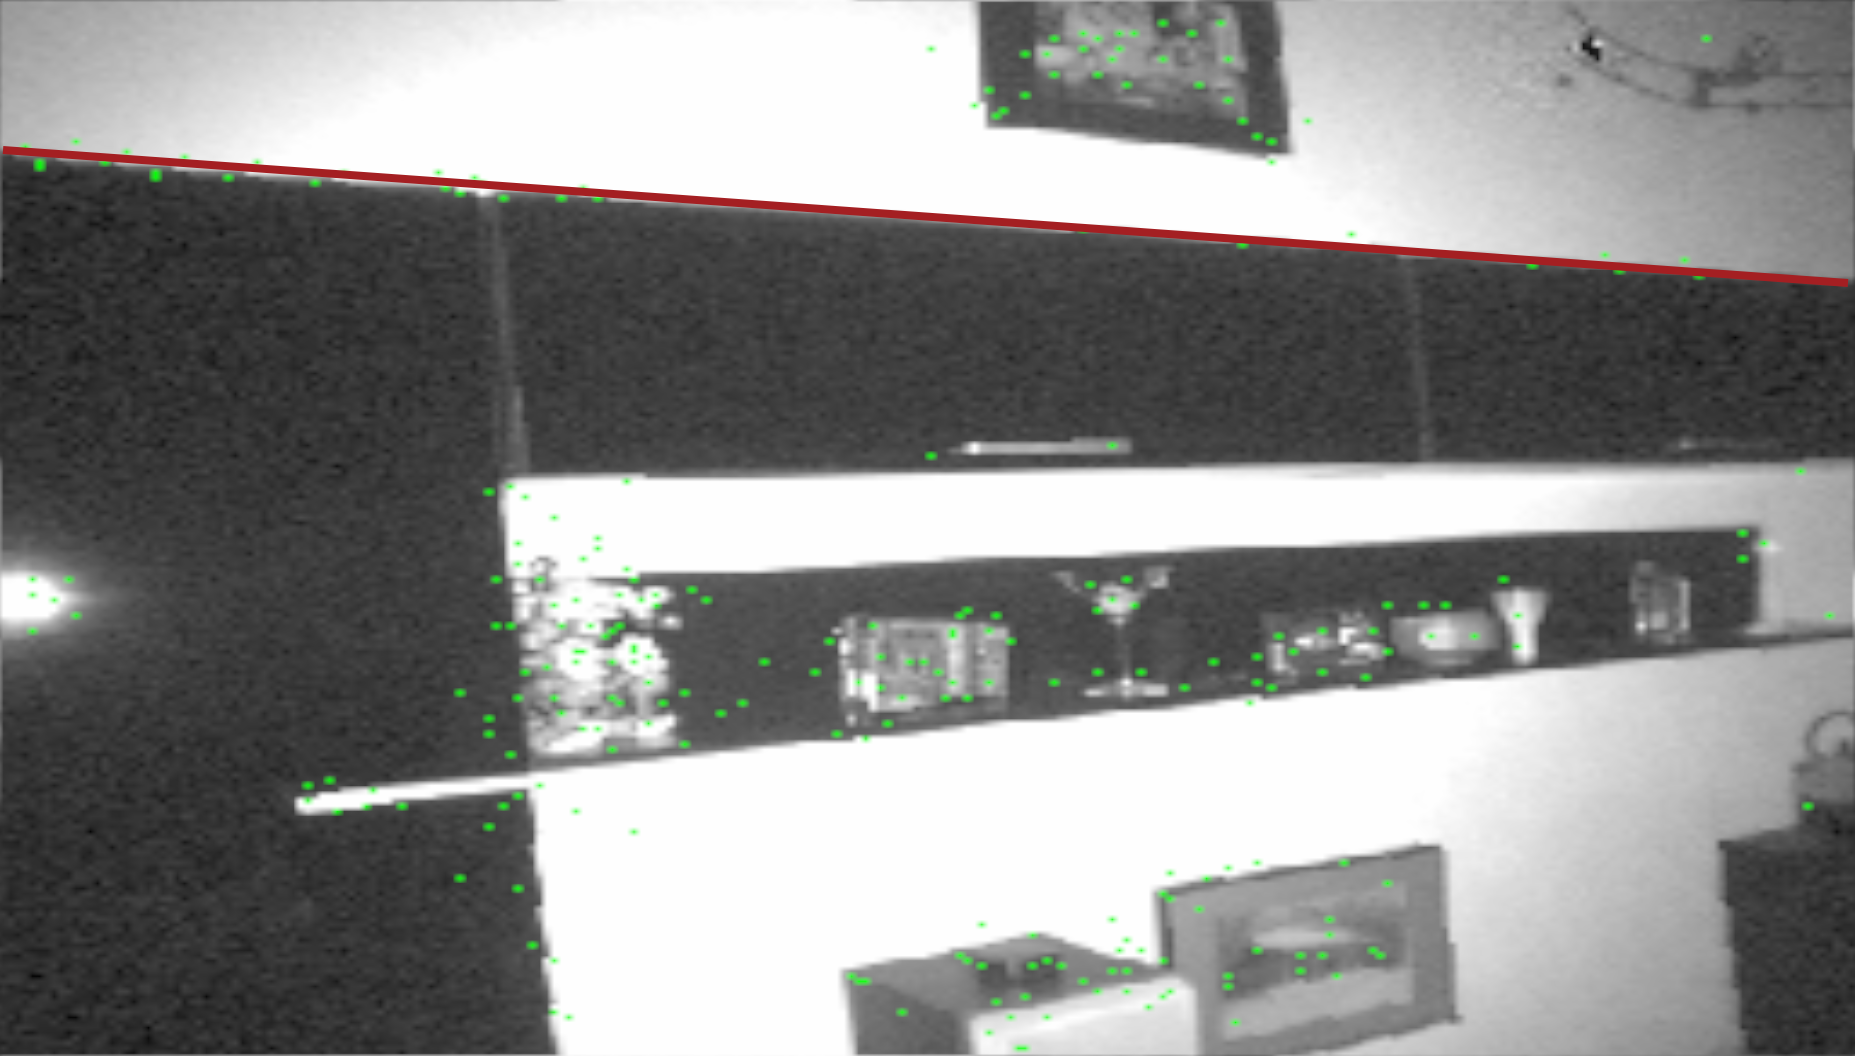
\includegraphics[scale=0.11]{images/cloud_3d_linearity_image.png}
      \subcaption{Image}
      \label{fig:linearity3d_image} 
    \end{minipage} % Hier darf keine Leerzeile zwischen den beiden Minipages liegen!
    \begin{minipage}[b]{0.47\textwidth}
      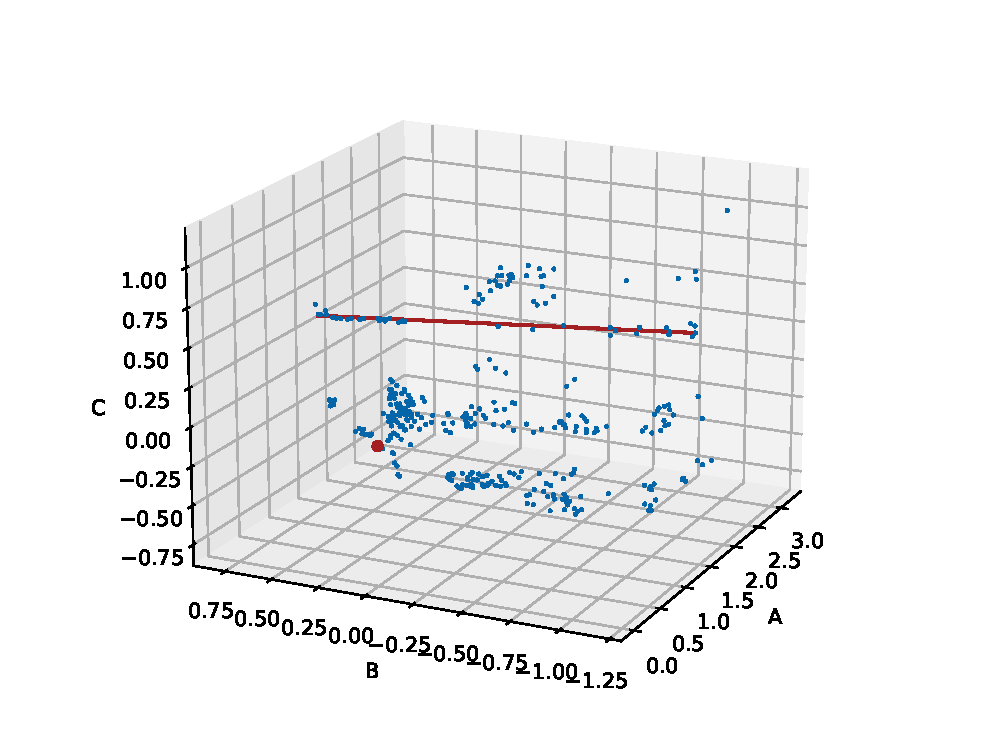
\includegraphics[scale=0.72, trim={3.3cm 3cm 3cm 3.5cm},clip]{images/linearity_3d.eps} 
      \subcaption{Cloud}
      \label{fig:linearity3d_cloud} 
    \end{minipage}
    \caption{The scene reconstruction from the left image to the full point cloud. The red line is equivalent in both figures. Each green dot in the left image is a SIFT feature. The red dot in the point cloud is the position of the camera.}
    \label{fig:linearity3d}
  \end{figure}

\subsection{RANSAC feature matching}
\label{sec:RANSAC_Results}
The RANSAC algorithm improves the quality of matched features over the flawed brute-force matcher. The data of the ToF camera is prone to noise, the RANSAC algorithm needs to cope with positional uncertainties. As discussed in Section \ref{sec:results_distance_meas}, the standard deviation in the $a$-axis is roughly 7mm, which also affects the mapping to the$b$- and $c$-axis from the 3d reconstruction.\\
A threshold based on the sum of square differences gives the RANSAC algorithm the flexibility to create suitable matches.
The SSD creates a sphere around the estimated position. The equation of a sphere of radius $r$ follows the equation $r^{2}=x^{2}+y^{2}+z^{2}$. Setting the radius $r$ equal to the standard deviation of 7 mm on the $a$-axis results in a threshold of around 0.00005. Statistically, around 68\% of the matches should reside inside this sphere of 14 mm diameter, however the number of matches is very small as seen in Figure \ref{im:noise_against_thresh} The error on the other axis is smaller as discussed in Section \ref{sec:results_distance_meas}, this does not explain the poor matching performance at this threshold, as seen in Figure . Likely, some other source of noise diminishes the matching performance. The image noise on the black-and-white image causes the extracted SIFT features jitter. Even a jitter in the range of 1 pixel easily leads - depending on its distance - to an error of more than a centimeter. On the other hand, to detect a lateral speed of 0.1 m/s at a frame rate of approximately 10 frames per second, a shift of 1 cm needs to be detected.
\begin{figure}[H]
    \centering
    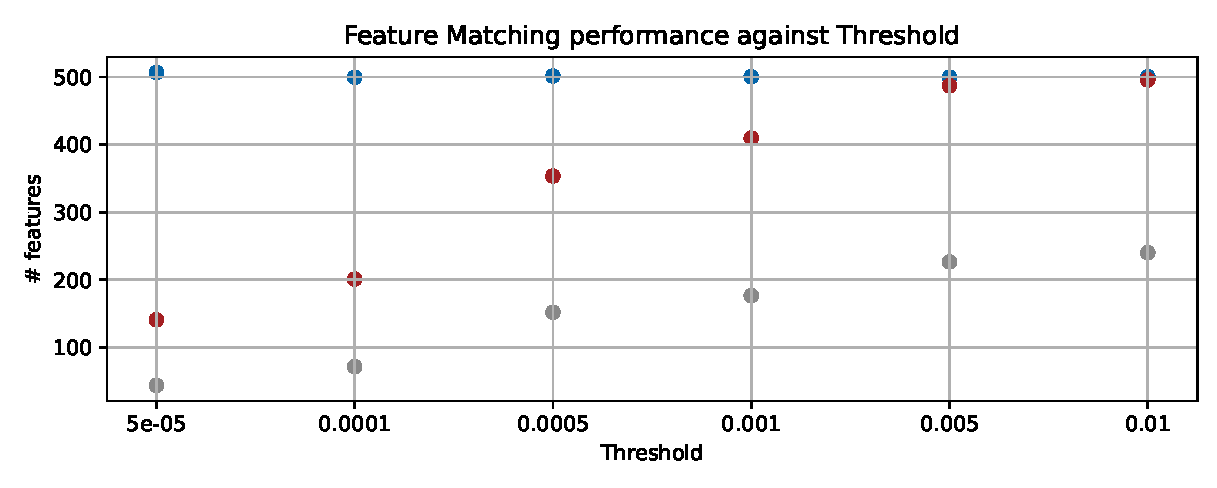
\includegraphics[width=1.0\textwidth]{images/noise_against_threshold.eps}
    \caption{Plotting the feature matching performance against different thresholds shows the quality of the RANSAC feature matcher. In blue, the raw number of unmatched features in each test, in gray the brute force matches and in red the RANSAC matches.}
    \label{im:noise_against_thresh}
\end{figure}
Higher tresholds in Figure \ref{im:noise_against_thresh} show the expected performance of the brute-force matcher in grey. The RANSAC feature detector vastly improves the matching performance, seemingly up to over 97\% at the threshold of 0.005. At a threshold of 0.005, the sphere around the expected position has more than 14cm in diameter, leading to the undesired situation of the RANSAC matcher finding feature points. The RANSAC matcher might find the same match for different unsuitable feature points. The matches are not exclusive, combined with a large threshold, it is likely that most features find a match.\\
The balance between the uncertainty and the requirements for detecting slow speeds lead to a chosen threshold of 0.0005. This threshold leads to a sphere of about 4.4 cm in diameter, which filters outliers.\\ 
Figure \ref{im:3d_features_rotation} on the next page demonstrates the matching with the chosen threshold at the example of a rotation of the camera head. Two consecutive frames generated a point cloud each. The estimated rotation and translation move each data point of one cloud to a hypothetical position. The closest data point of the other cloud around this hypothetical position is accepted if it lies within a sphere of 4.4cm diameter. 
After another calculation, these matched data points lead to the optimal rigid motion, discussed in the following sections.\\
\begin{figure}[H]
  \centering
  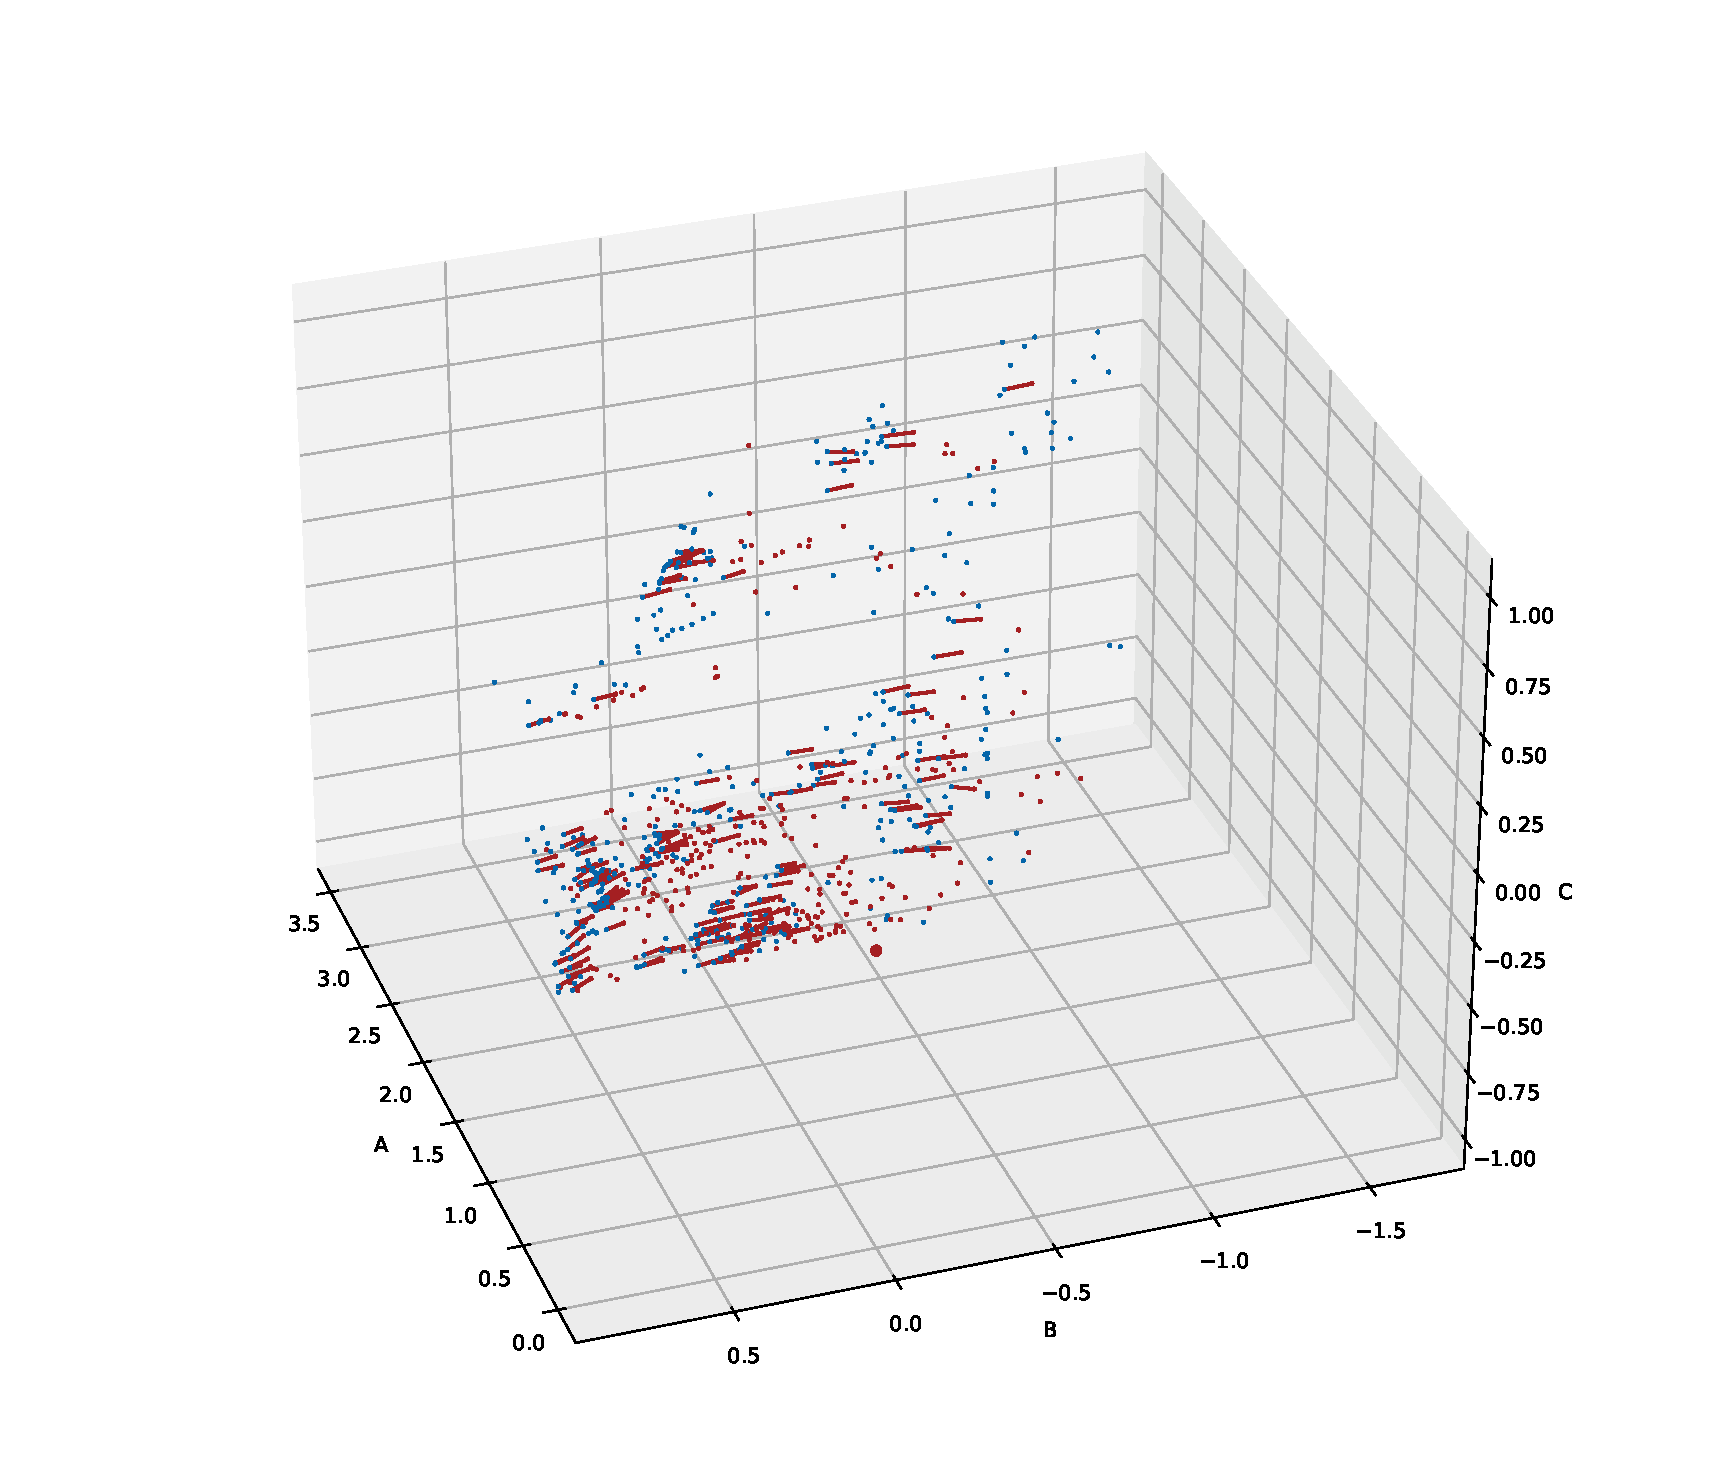
\includegraphics[width=1.0\textwidth,trim={7cm 7cm 8cm 5cm},clip]{images/3d_features_rotation.eps}
  \caption{Two raw point clouds with the found matches connecting them. The camera is rotated in between the frames, which leads to the displacement of the point cloud. The connecting lines are roughly 10cm long, depending on the position. The large red dot in the foreground is the position of the camera.}
  \label{im:3d_features_rotation}
\end{figure}
\begin{table}[ht] \centering
	\begin{tabular}{|p{5cm}|p{3cm}|p{3cm}|p{3cm}|} \hline
		\rowcolor{gray} Measurement & Rotation & Translation X & Translation Y \\
		\hline
		Total Features (avg) & 435.9 & 400.0 & 488.4\\
		\hline
		Brute-Force Matches (avg) & 117.9 & 104.2 & 112.6  \\
		\hline
		RANSAC Matches (avg) & 280.2 & 262.5 & 284.3  \\
		\hline
	\end{tabular}
	\caption{Per-Frame average performance of the feature matching approaches}
	\label{tab:ransac_performance}
 \end{table}
 The claimed performance for the brute-force matcher is below 50\% when applied to two identical images, according to the developers of the CudaSift library.\cite{cudaSiftRepo} On noisy frames, even with motion between frames, the quality is expected to be lower.\\
 Table \ref{tab:ransac_performance} shows the performance of the RANSAC implementation in comparison to the brute-force matcher. On average an improvement of over 100\% in the number of accepted matches is achieved by running the three-dimensional RANSAC algorithm.


\subsection{Rotation from ToF camera}
\label{sec:results_tof_rotation}
Both the gyroscope and the ToF rotation generate rotation speeds and are both converted into rotation quaternions. Transforming the rotation speed to a quaternion allows direct comparison of the two sensory systems. Analyzing the imaginary parts is sufficient, as explained in Section \ref{sec:RotationQuaternion}.
In this experiment, the camera head was rotated in each direction and directly compared to the gyroscope data. The camera was mounted on a standard camera tripod and rotated by hand, as the author has no access to a device allowing automated rotations. Figure \ref{im:tof_rotation_measurement} shows the results. 
\begin{figure}[H]
  \centering
  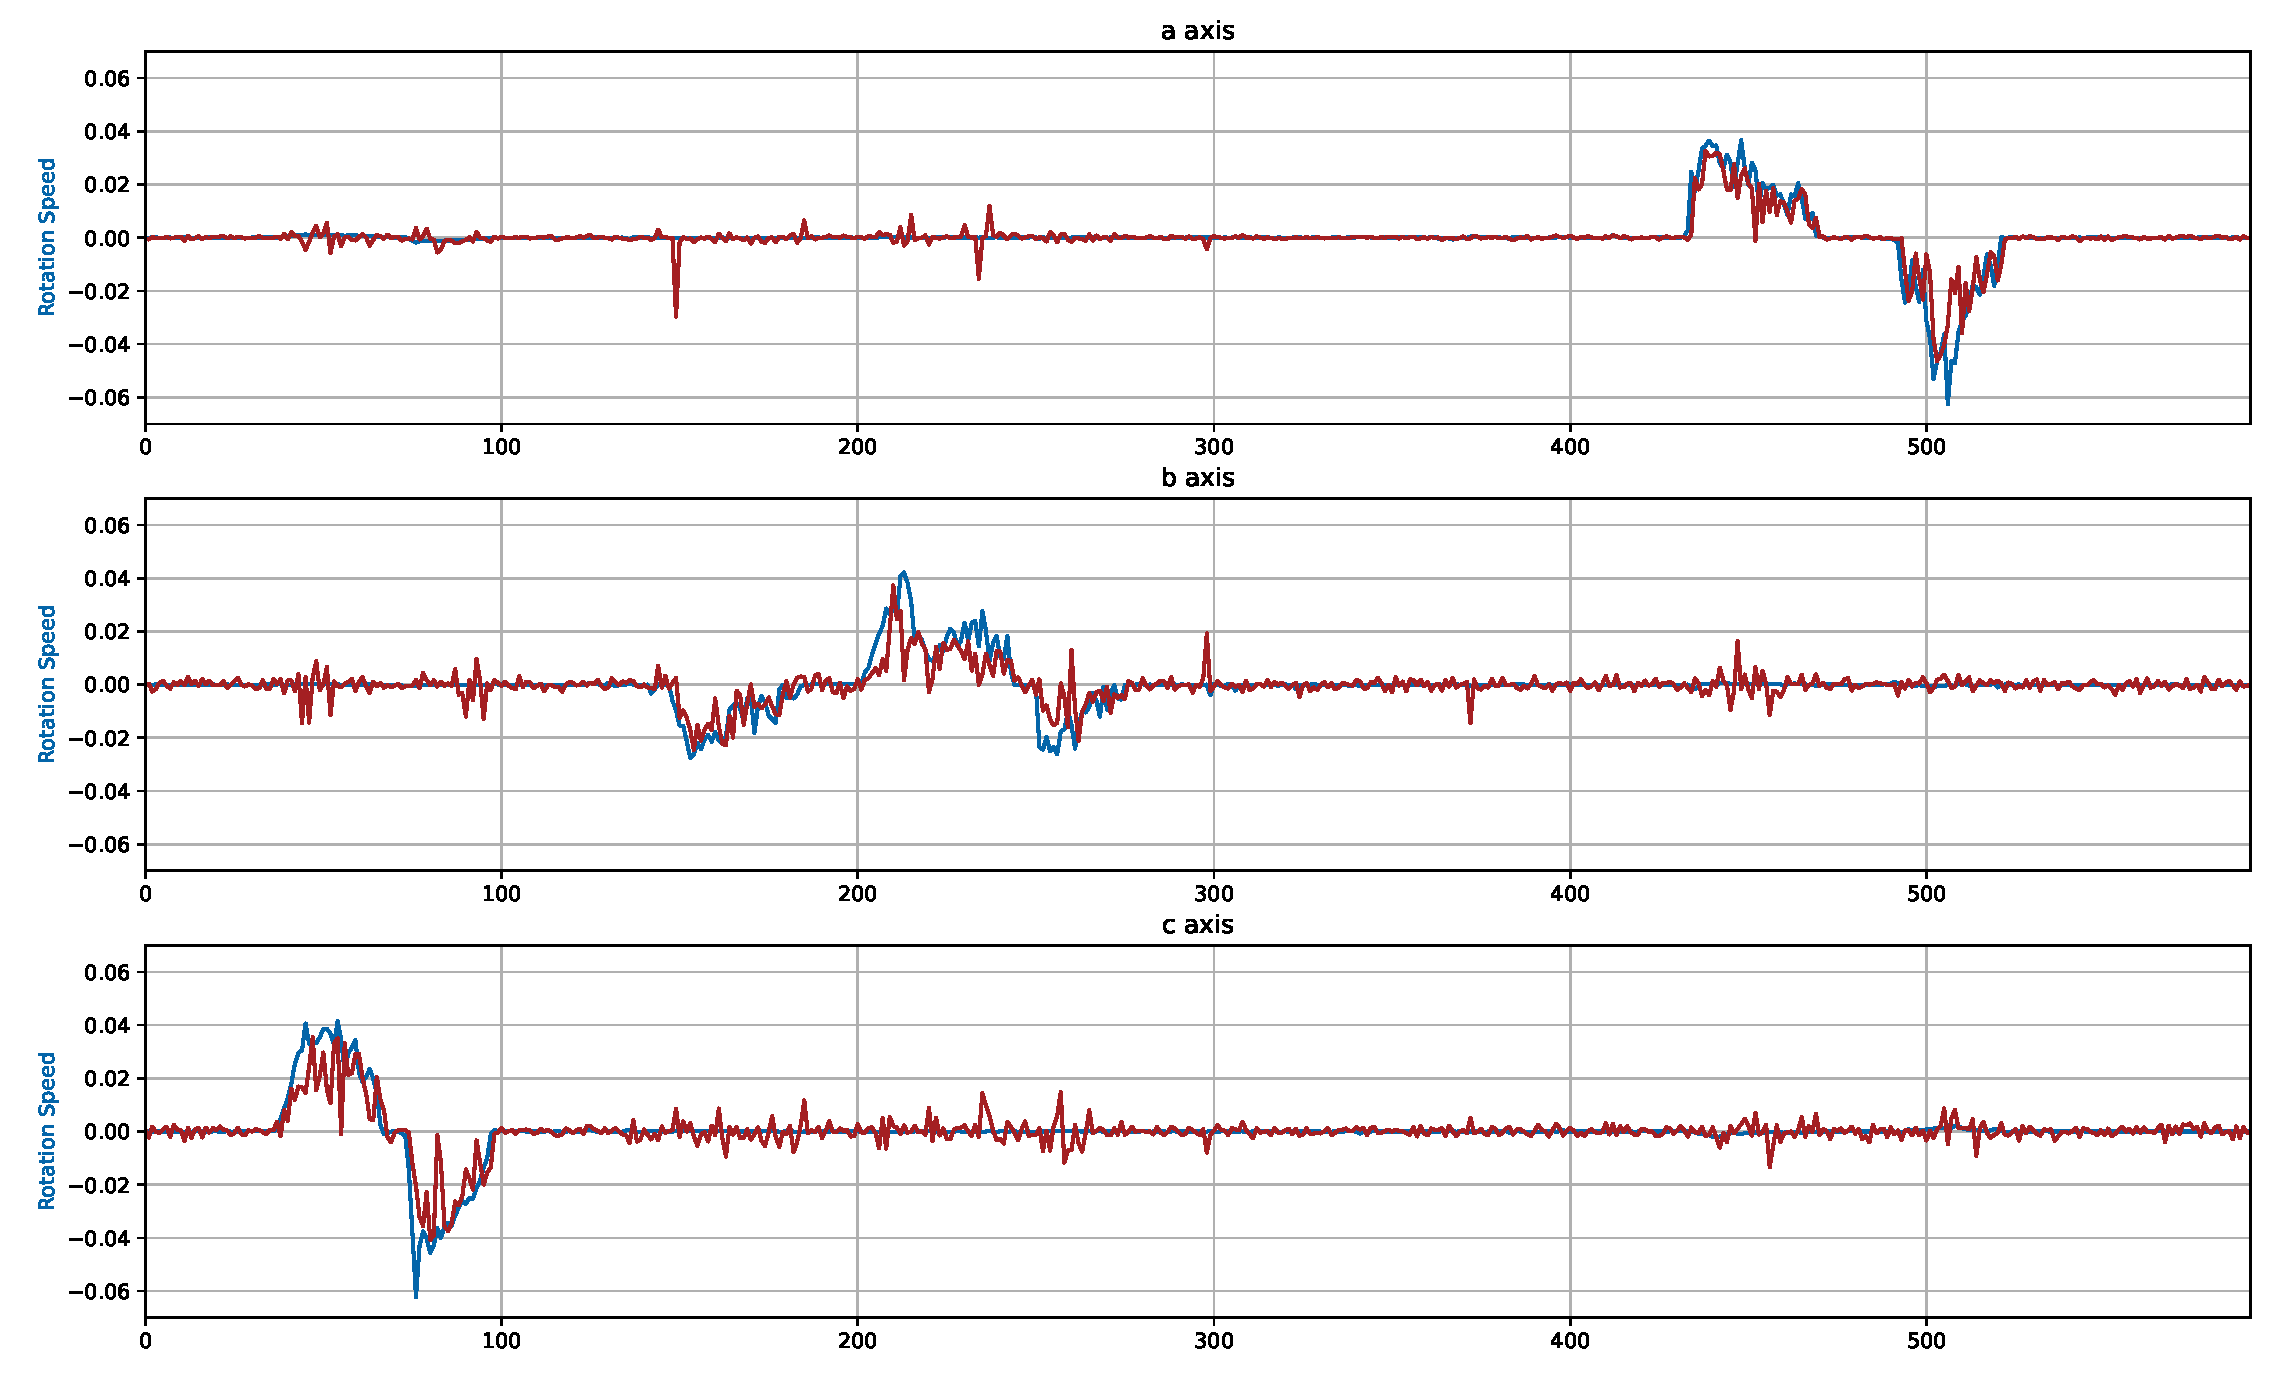
\includegraphics[width=1.0\textwidth]{images/tof_rotation_measurement.eps}
  \caption{The individual axis of the ToF rotation quaternion in red plotted against the gyroscope quaternion in blue. The camera head got rotated in each direction after another, first sideways around the $c$-axis, then downwards and upwards around the $b$-axis and at last tilted around the $a$-axis. The plotted values resemble imaginary parts of a quaternion and are therefore without units.}
  \label{im:tof_rotation_measurement}
\end{figure}
The measurement on the motion estimation from the ToF camera shows significant noise, especially on the rotation alongside the b- and c-axis, and does not entirely follow the gyroscope curve in blue. Nevertheless, measurement shows the proof of concept.
\subsection{Translation from ToF camera}
\label{sec:translation_tof_rotation}
Like for the rotation measurement, the translation is measured against the IMU. In the case of translation, the acceleration data from the IMU is compared to the translation estimation of the ToF camera. The camera is moved on a toy rail in $x$- and $y$-directions. Motion along the $z$-axis is not measured, as its priniciple is the same as for the $y$-direction. The translation cannot be measured in one take as the railway needs to be moved for the different axis.\\
Alongside the $x$-axis, the camera moves closer to the objects in the viewfinder, alongside the $y$-axis, the camera moves perpendicular. Note that these measurements are already in $xyz$-notation, as the orientation was corrected. As the camera did not rotate during these measurements, the values are equivalent to the $abc$-notation. The camera was slid from its origin to the front, respectively to the side, and to its origin twice on each run. The first motion was kept fast, the second motion was kept slow. The length of the track is about 0.5 m in both directions.\\
As visible in the Figures \ref{im:tof_translation_measurement_x} and \ref{im:tof_translation_measurement_y} on the next page, the velocity data from the ToF camera shows significant noise, but the motion is detected correctly.
\begin{figure}[H]
  \centering
  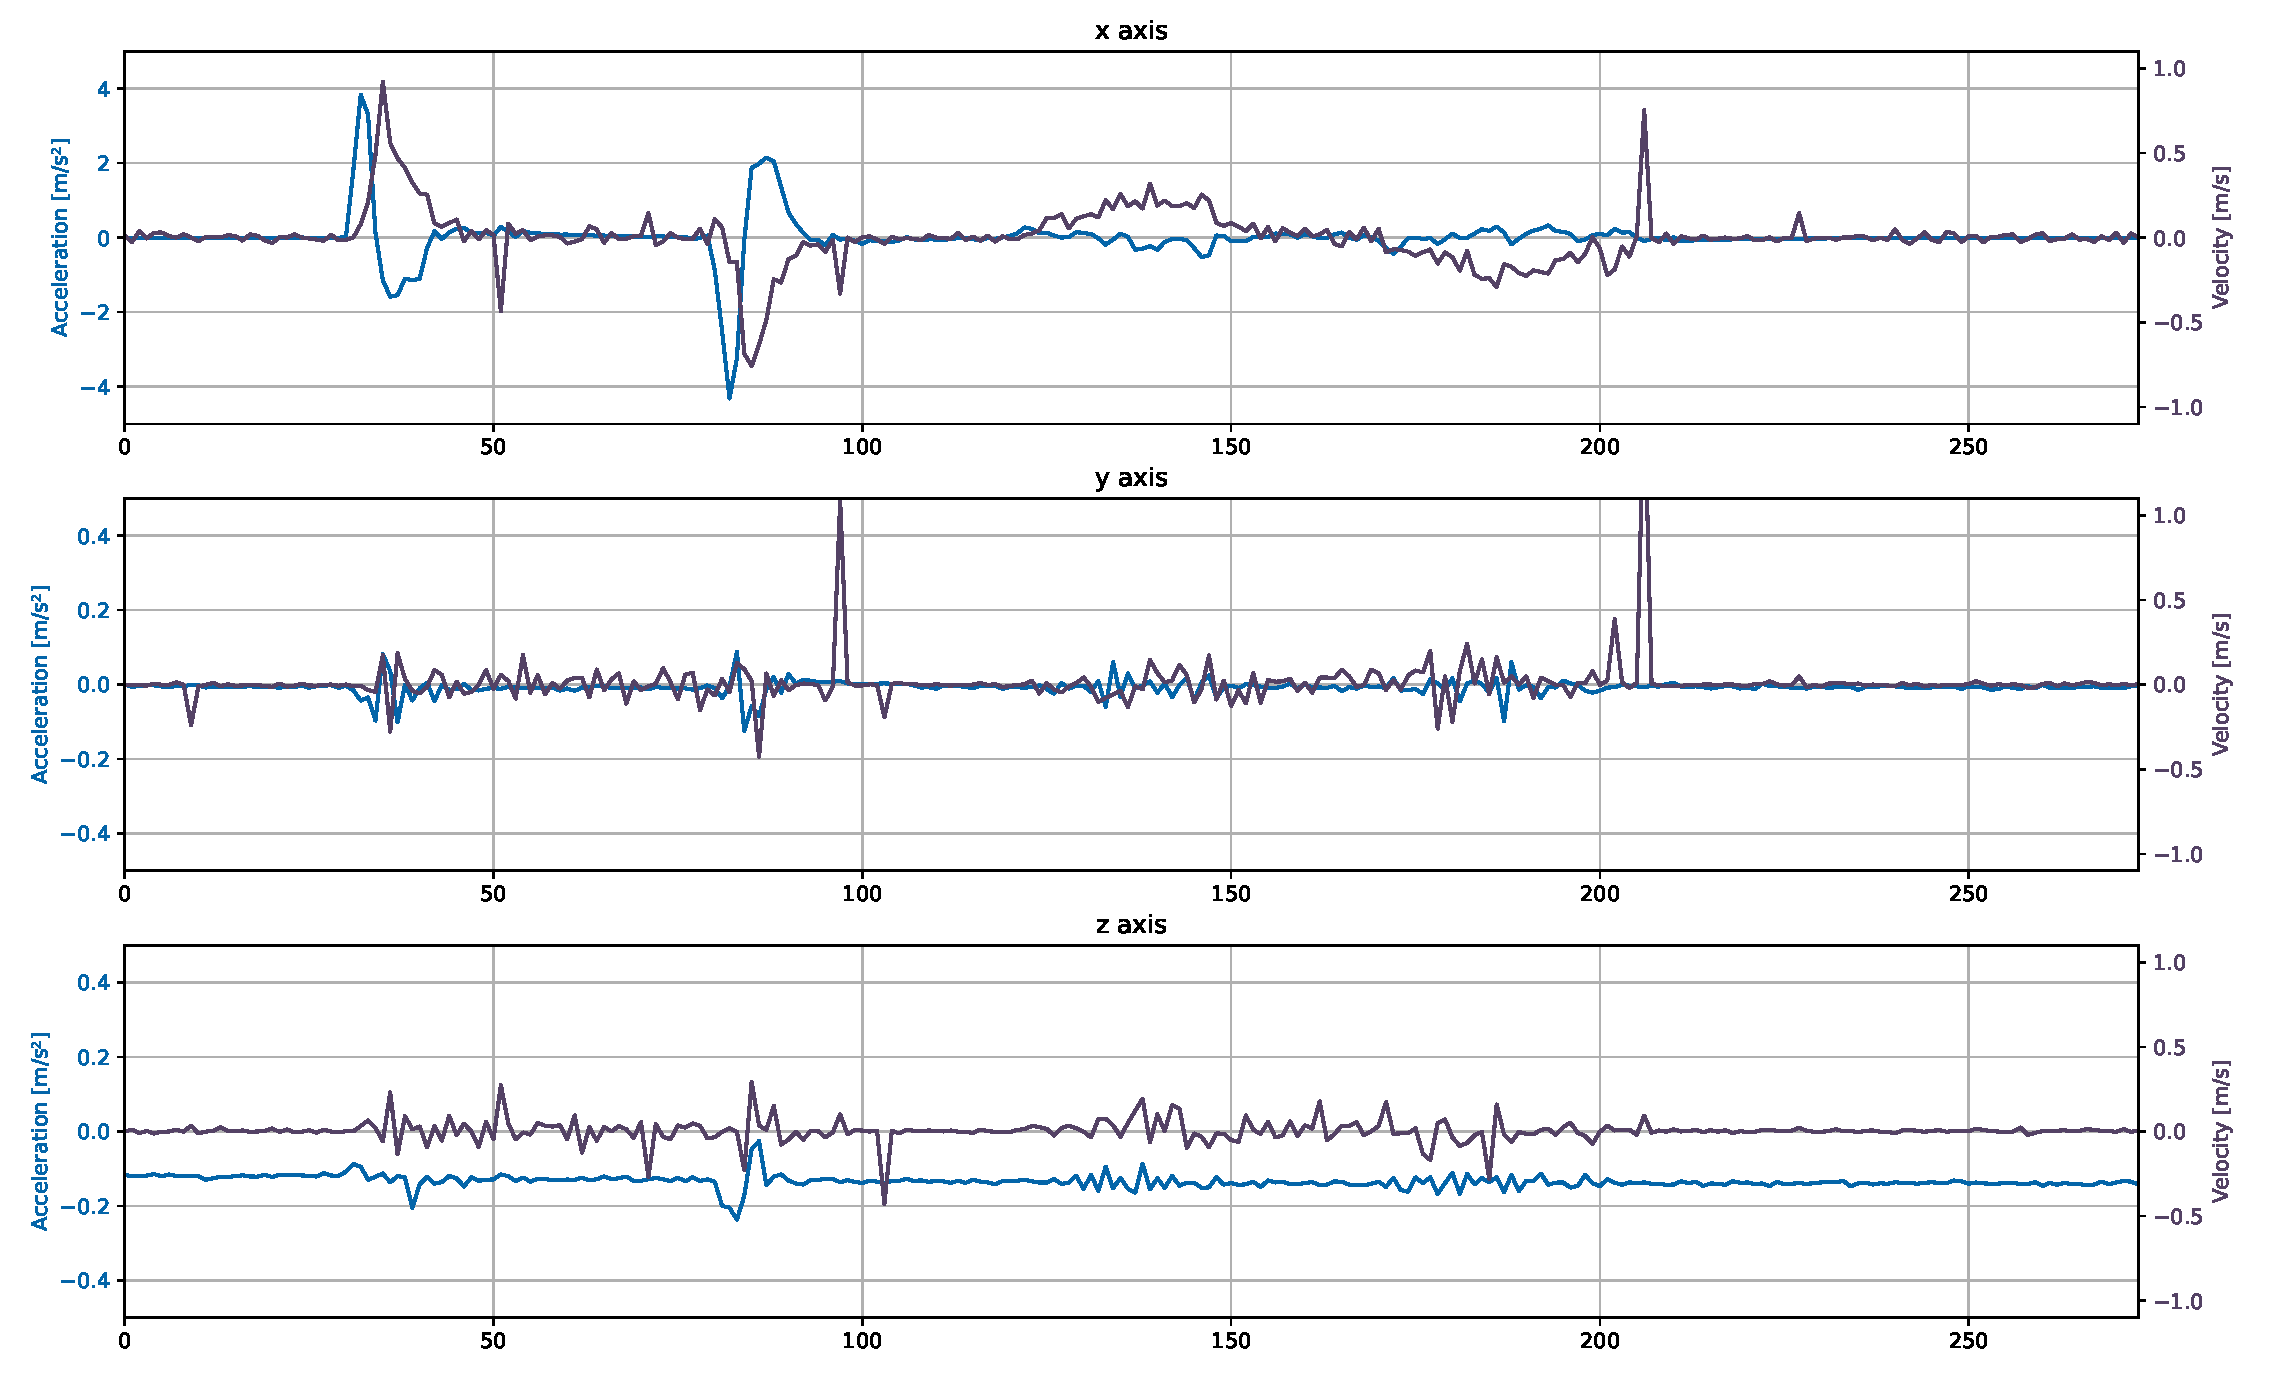
\includegraphics[width=1.0\textwidth]{images/tof_translation_measurement_x.eps}
  \caption{Raw measurement of the translation alongside the x-axis. Before and around frame 50, the camera is slid fast forward, kept in pause just to slide back before reaching frame number 100. After frame 100 and before frame 220, the same motion is repeated but slower. Blue is the acceleration from the IMU and purple the velocity from the TOF sensor.}
  \label{im:tof_translation_measurement_x}
\end{figure}
\begin{figure}[H]
  \centering
  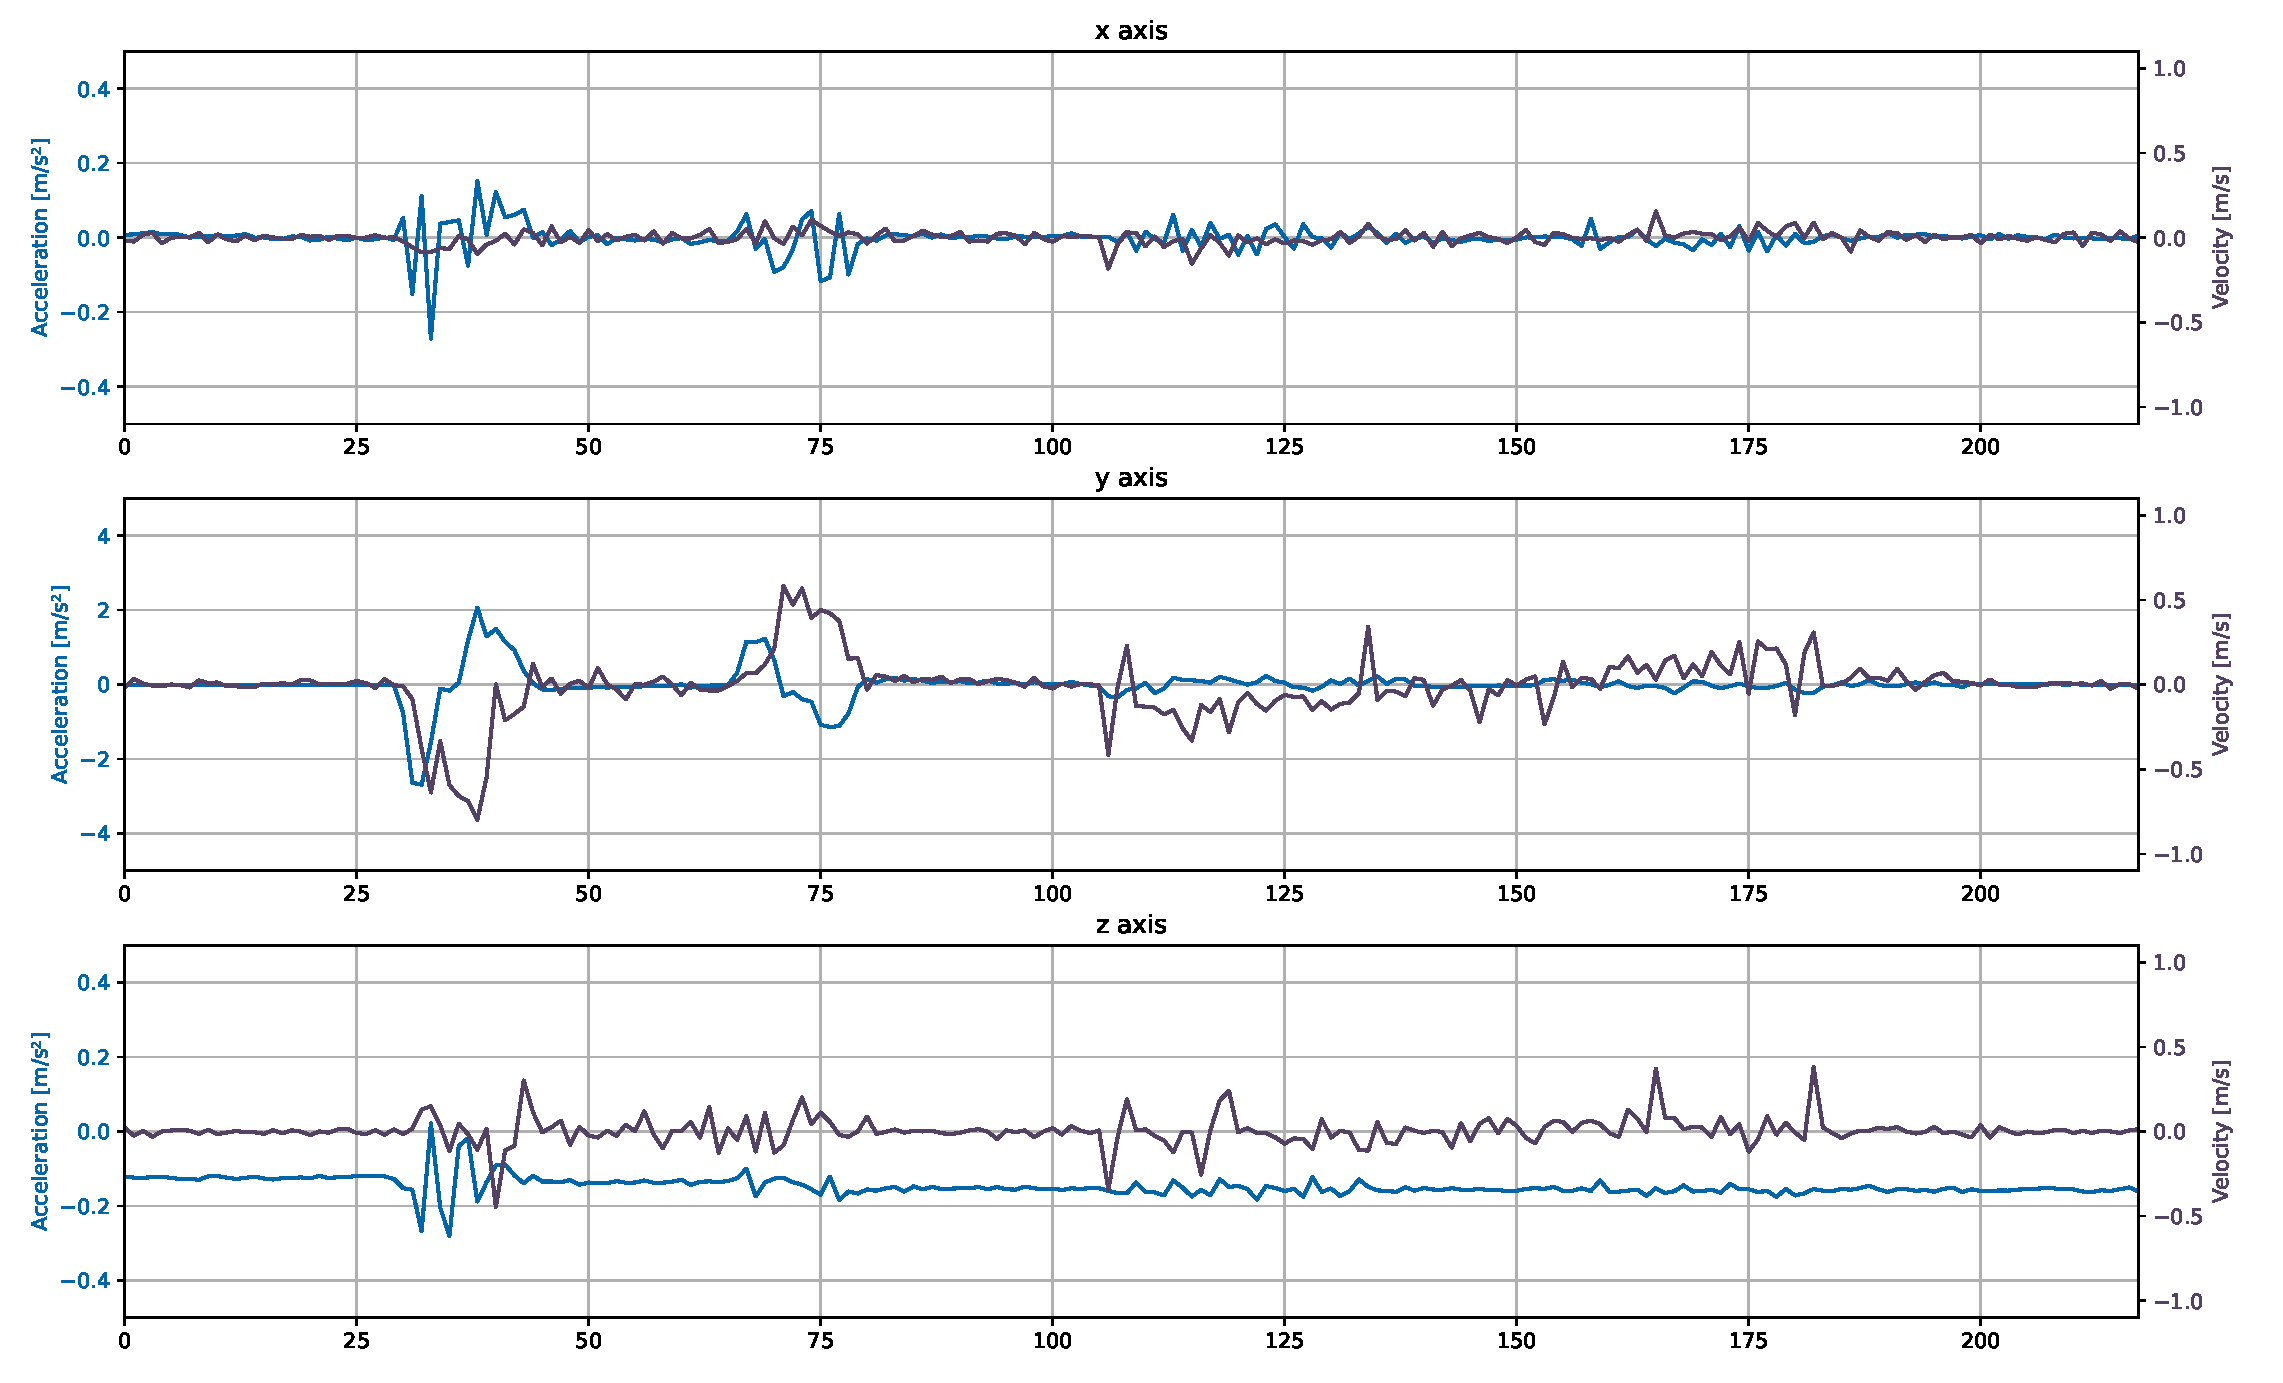
\includegraphics[width=1.0\textwidth]{images/tof_translation_measurement_y.eps}
  \caption{Raw measurement of the translation alongside the y-axis. Between the frames 25 and 50, the camera is slid to the right, kept there and slid back to the origin around frame 75. The motion is repeated slower after frame 100 and before 200. Blue is the acceleration and purple the velocity. Note how noise increased on the other axis, while the camera was in motion.}
  \label{im:tof_translation_measurement_y}
\end{figure}
Raw integration of the ToF velocity values gives insight into the measurement's quality. As visible in Figure \ref{im:tof_translation_measurement_integrated}, the data reconstructs the linear motion in both directions, even though it gets jagged by noise as expected. Noteable outliers, like at the end of the second motion on the x-axis, induce larger errors. 
\begin{figure}[H]
  \centering
  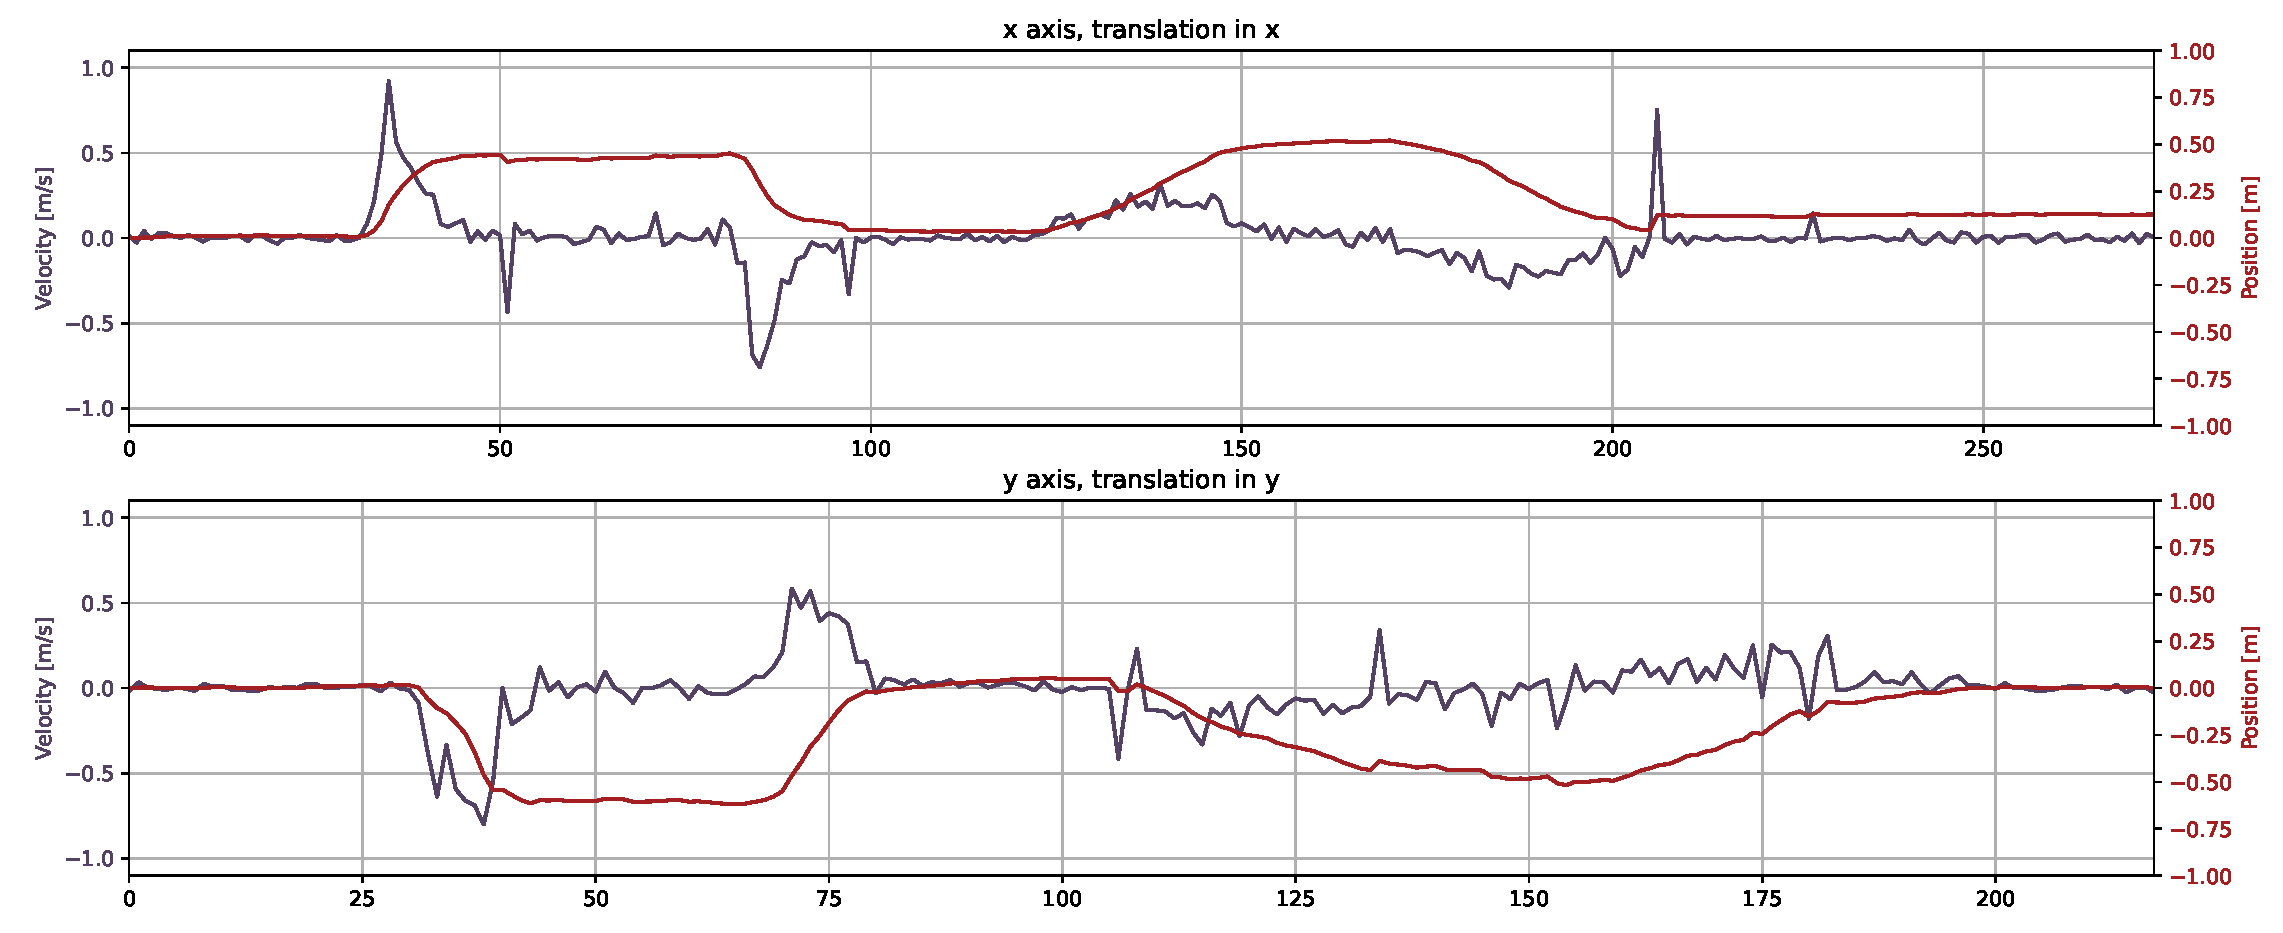
\includegraphics[width=1.0\textwidth]{images/tof_translation_measurement_integrated.eps}
  \caption{Raw integration of the relevant axis in both translations of the ToF velocity data. Purple is the velocity from the ToF camera and red its integration.}
  \label{im:tof_translation_measurement_integrated}
\end{figure} 
\section{Inertial Measurement Unit}
\label{sec:IMU_results}
The IMU contains a gyroscope and an accelerometer, whose data inputs the Kalman filter. While the comparison to the rotation estimation from the ToF camera already covered the gyroscope in Section \ref{sec:results_tof_rotation}, the accelerometer data requires more profound analysis.
\subsection{Accelerometer}
\label{sec:accel_results}
An accelerometer within the gravitational field of the earth will always measure the earth's gravitational pull in addition to other accelerations. The accelerometer needs calibration on each axis to compensate for the gravitational force, so the subtraction of $\vec{g}$ works in any orientation. Experimentation with the accelerometer showed that a hysteresis did prevent the accelerometer from reaching zero or $\vec{g}$ when standing still, depending on prior rotation. The hysteresis leads to a tiny offset on the acceleration, which causes an integrated velocity and devastatingly affects the further integrated position, as visible in Figure \ref{im:accelometer_integrated} on the next page. The aforementioned offset is visible \ref{im:tof_translation_measurement_x} and \ref{im:tof_translation_measurement_y} on the z-axis, thanks to the narrowed scale.\\
The added offset error worsens the drift compared to the simulation in Section \ref{sec:Kalmanfilter} dramatically. The integration to the velocity draws a smoother curve, than compared to the raw data of the ToF camera, but a drift is present. The third row of Figure \ref{im:accelometer_integrated} shows the critical drift, if the gravitational pull is not compensated entirely. The data for the third plot was recorded during the measurement of the motion alongside the x-axis.
\begin{figure}[H]
  \centering
  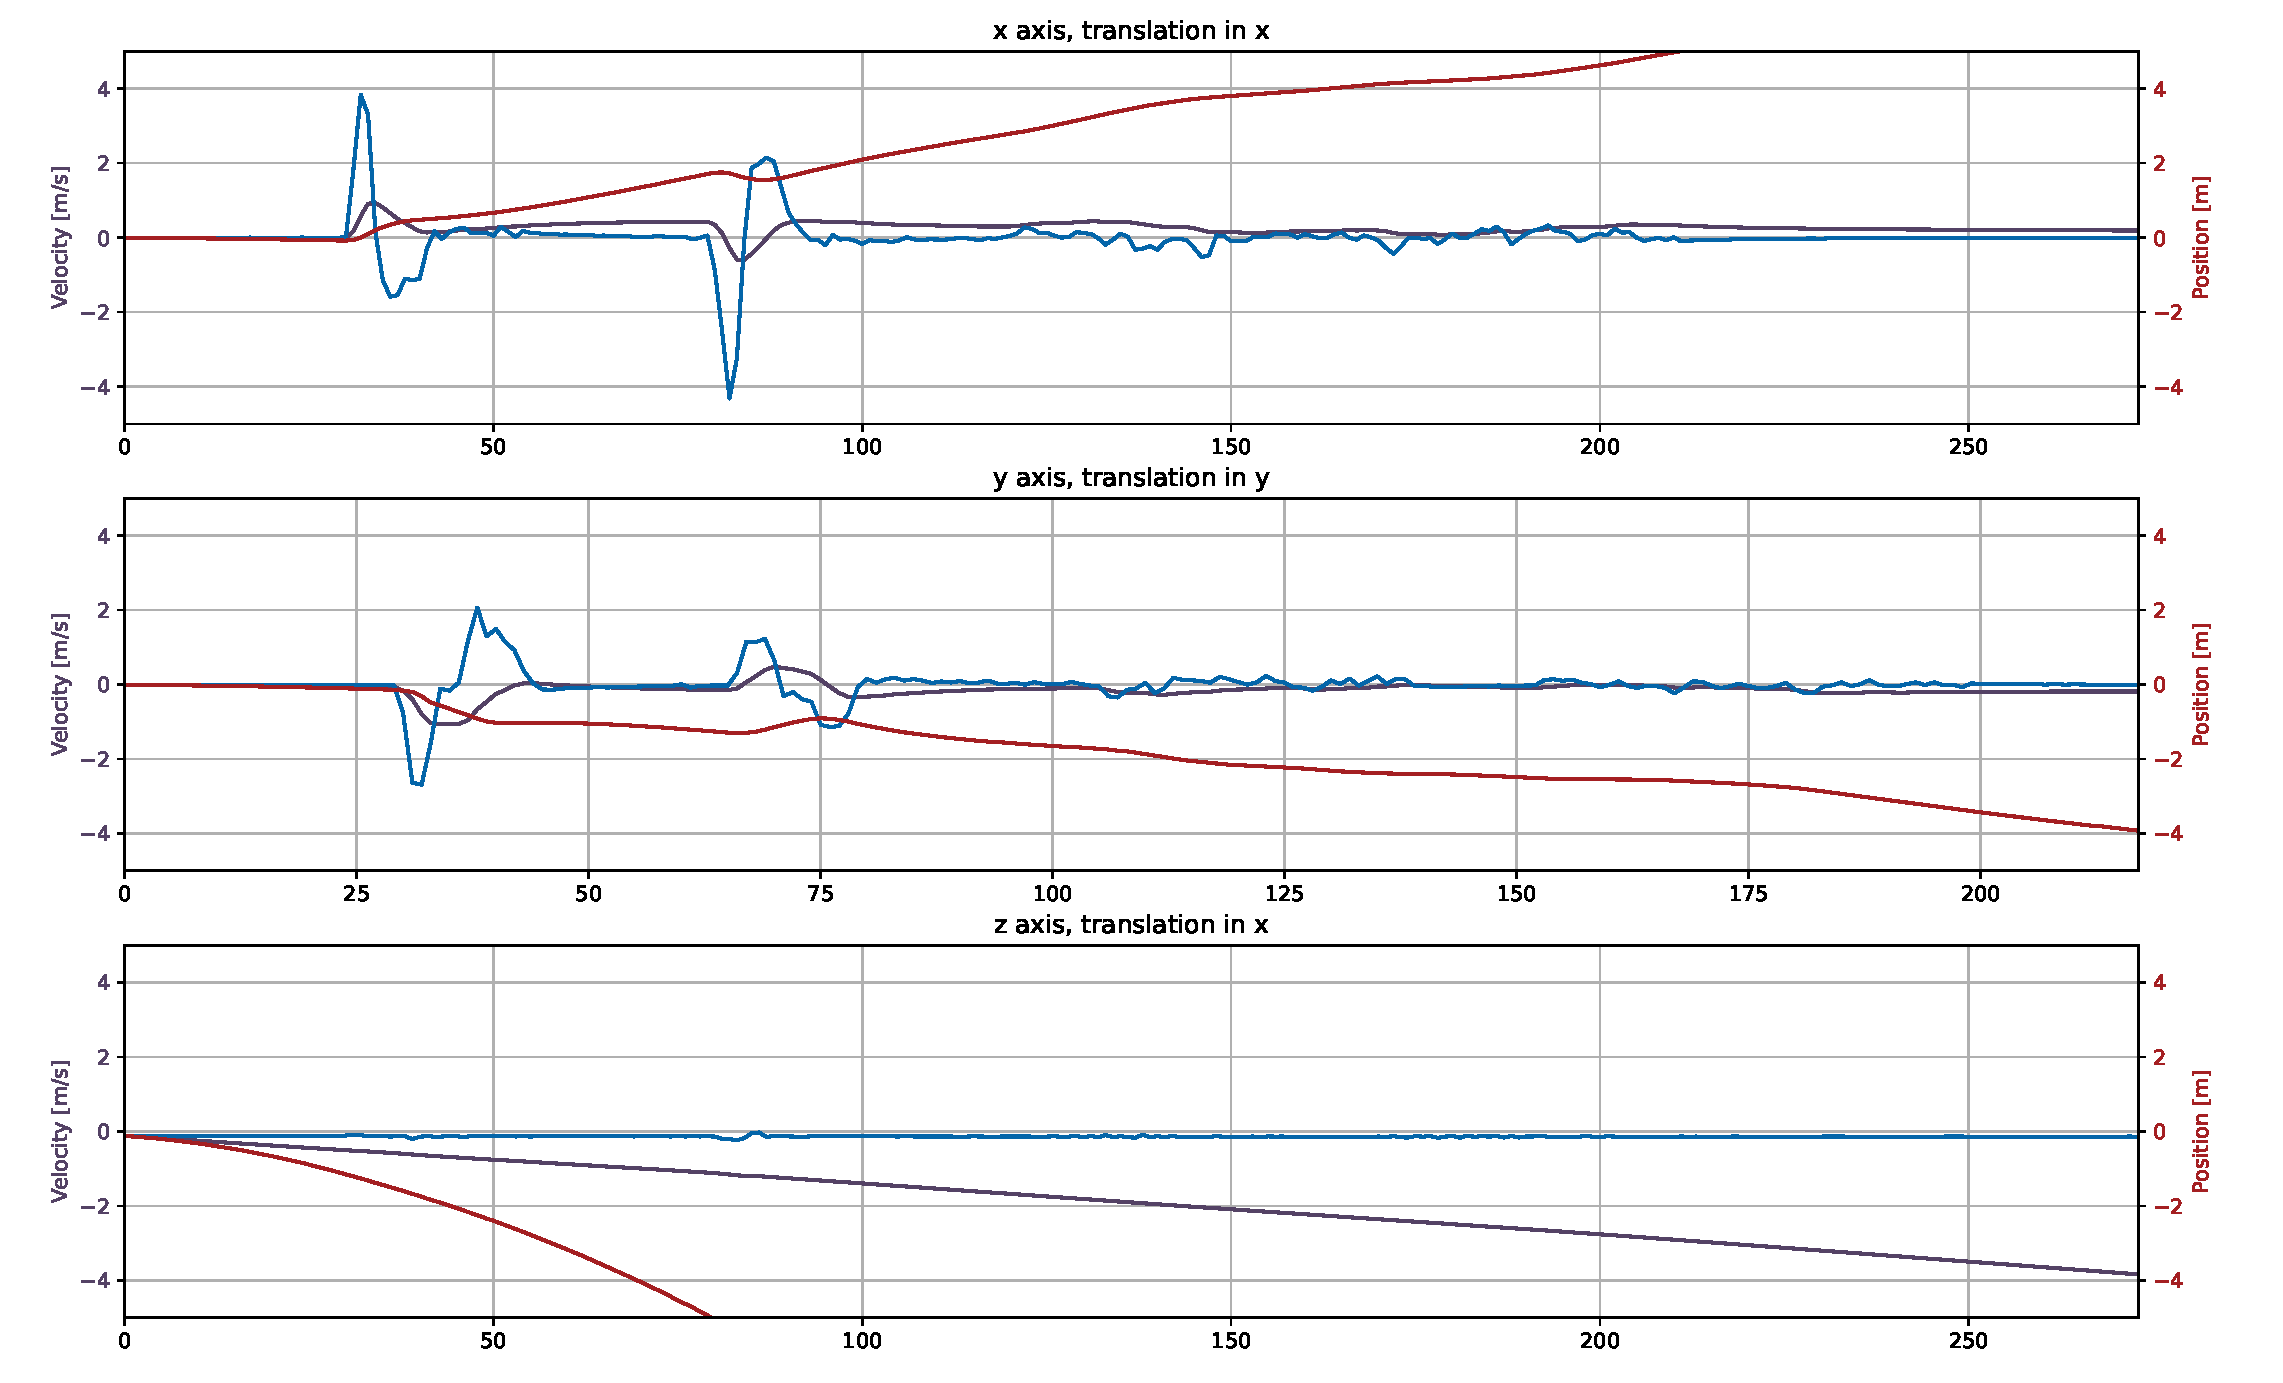
\includegraphics[width=1.0\textwidth]{images/accelerometer_translation_drift.eps}
  \caption{Integrations of the accelerometer data alongside relevant axis in both translations. Blue is the acceleration, purple the velocity (single integration) and red the position (double integration).}
  \label{im:accelometer_integrated}
\end{figure} 
\section{Kalman Filter}
\label{sec:kalman_results}
The Kalman filter combines the known motion model of the camera head with the measurement uncertainties and the raw input data from the ToF camera and the IMU. The only coupling between the rotation and the translation is the transformation from ABC-coordinates to the XYZ-space.
\subsection{Rotation}
\label{sec:kalman_rotation_results}
As mentioned in Section \ref{sec:results_tof_rotation}, the gyroscope and the ToF camera generate a rotation speed of comparable magnitude and shape. The gyroscope data is less distorted by noise, therefore the motion model can rely more heavily on this data source.\\
The Kalman filter smoothes data for the rotational speed through its model function and calculates the rotation from there. Additional to the gyroscope and the ToF camera, the drift compensation with the accelerometer stabilizes the values when the camera head is stationary.\\ 
In the comparison of the output of the Kalman filter against the sensory data, the strong weight towards the gyroscope becomes apparent, as shown in Figure \ref{im:meas_kalman_rotation}.\\
The shown result in Figure \ref{fig:rotation_demo} of the whole pipeline using only rotation data helps estimate the result's quality. The three rotation axes of the camera tripod do not intersect with the recording Raspberry Pi camera, thus, the 3D object moving in the image was expected. While the gyroscope's rotation axes intersect in the housing of the IMU, the axes of the ToF camera intersect at the optical center of the lens. For better accuracy, these sensor- and camera displacements on the camera head require additional compensation. 
\begin{figure}[H]
  \centering
  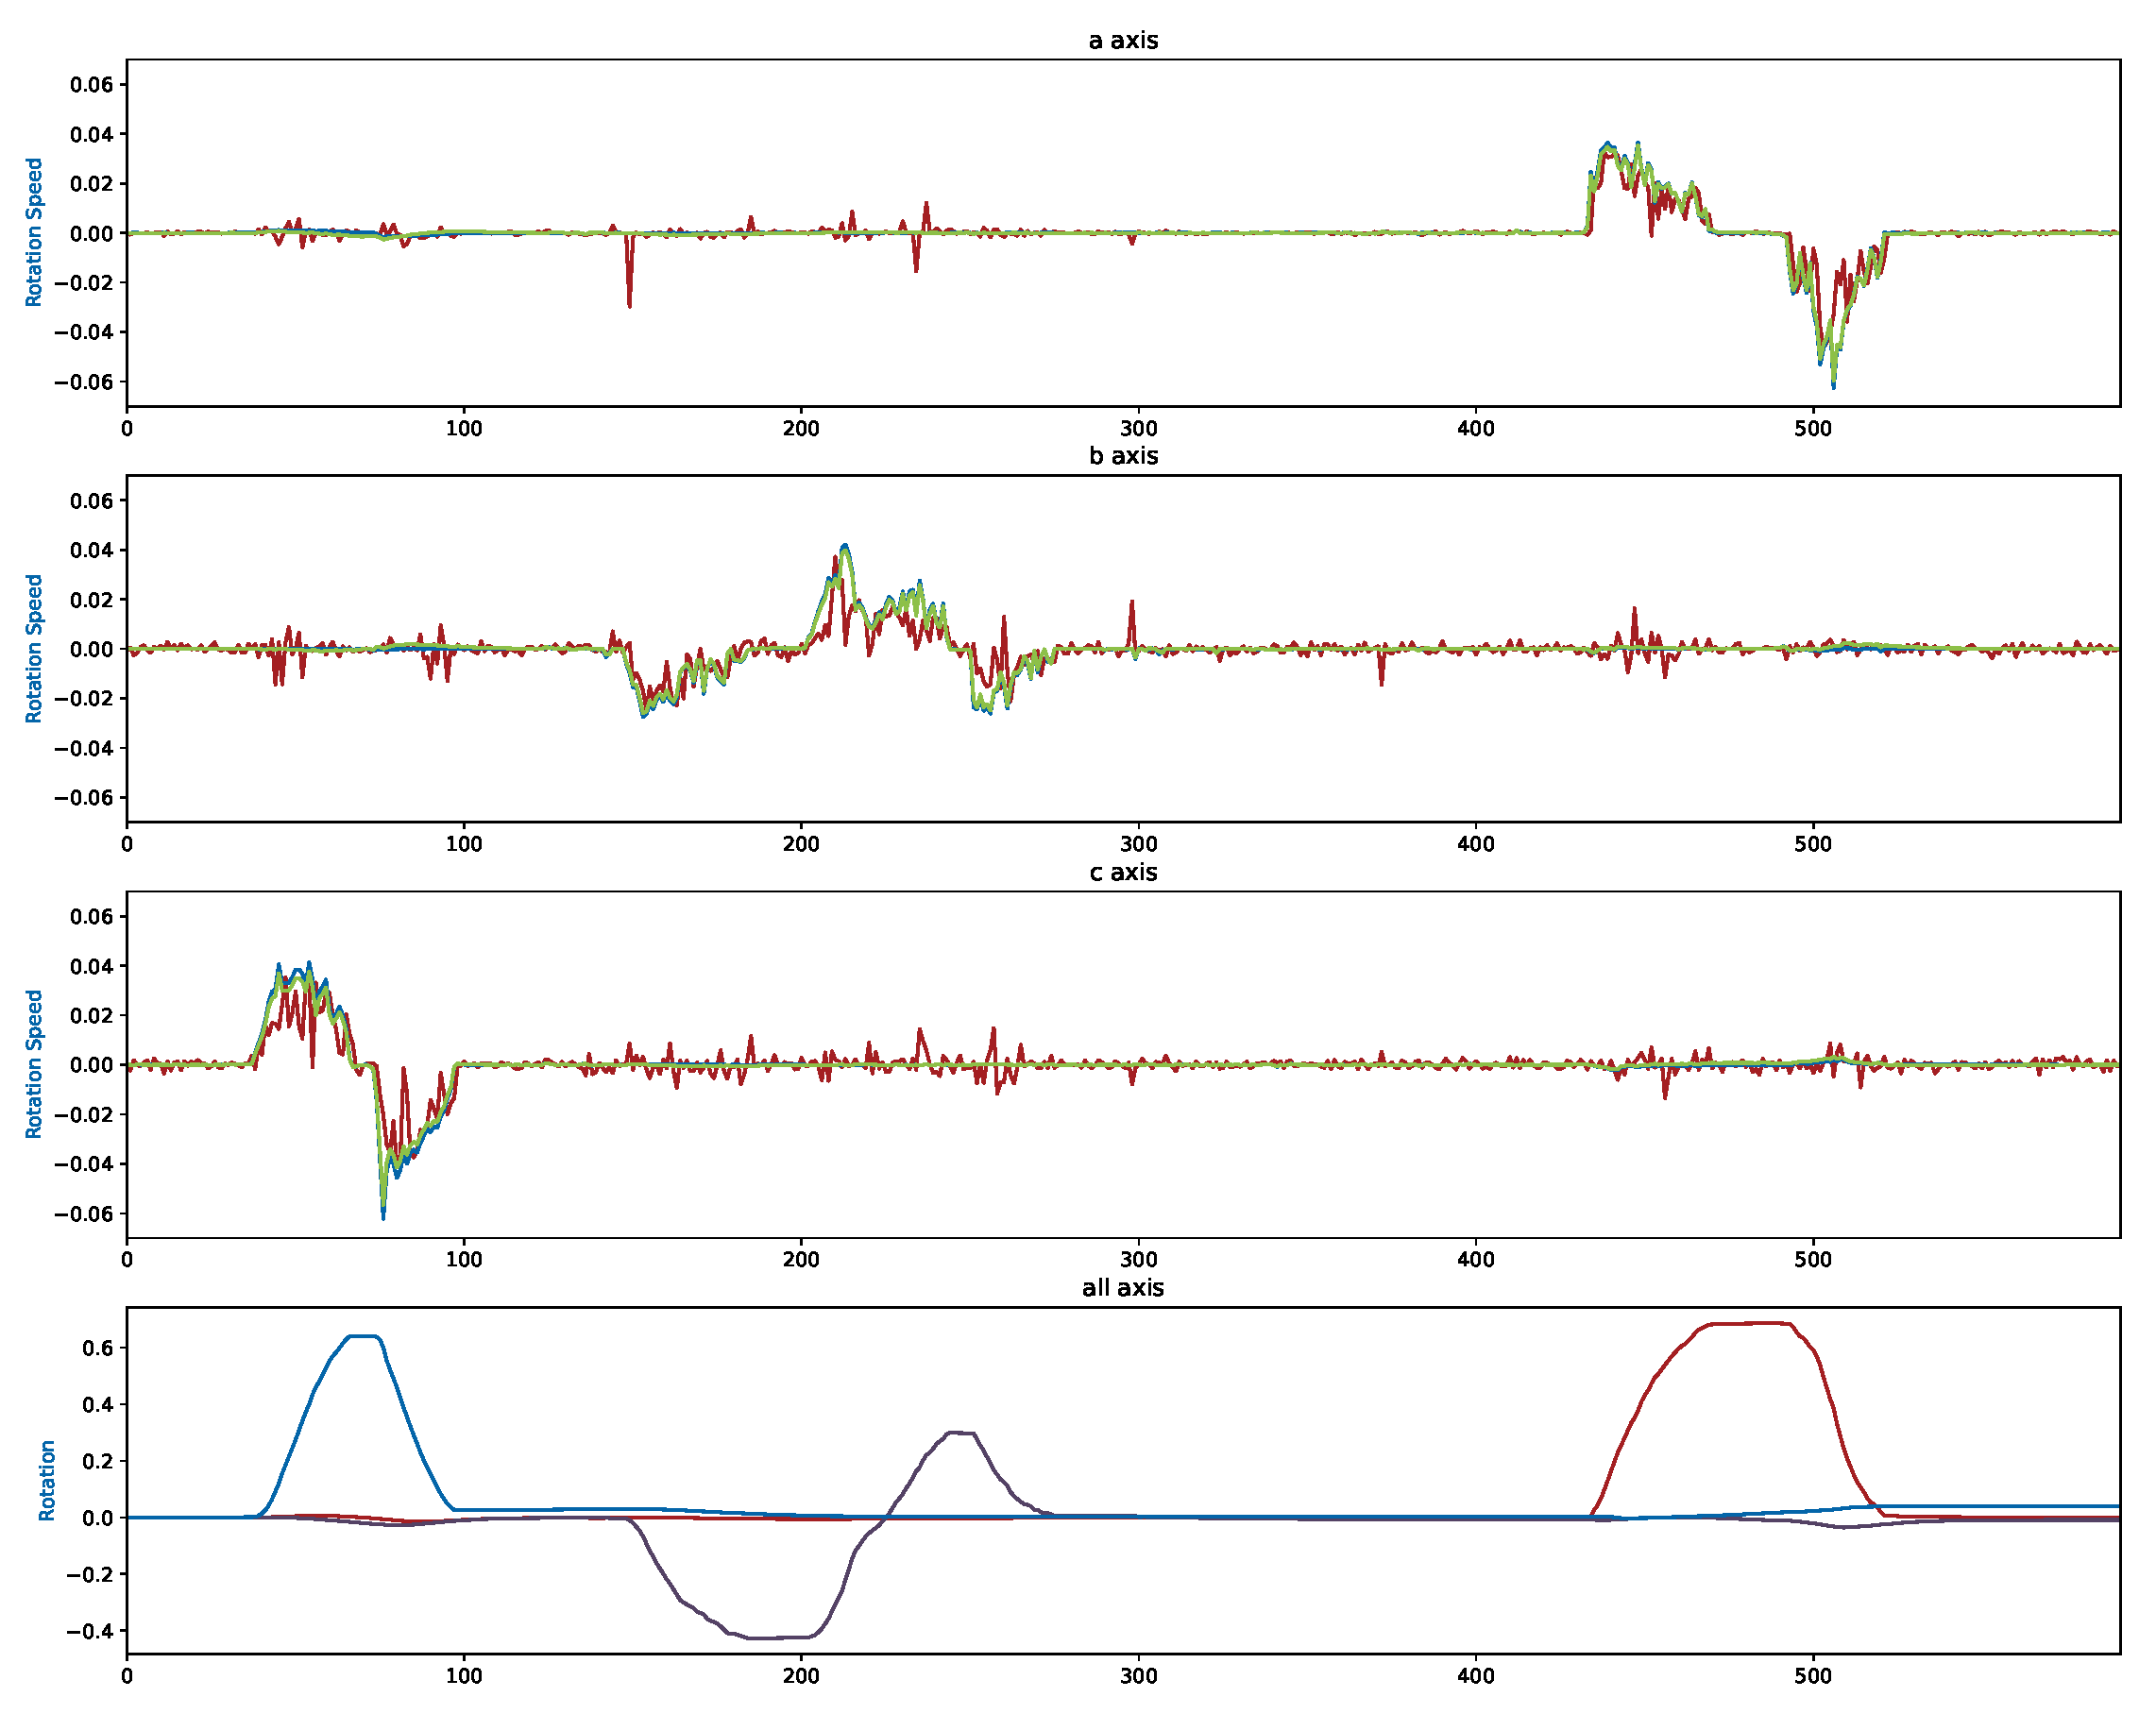
\includegraphics[width=1.0\textwidth]{images/meas_kalman_rotation.eps}
  \caption{The output of the Kalman filter is plotted in green, against the gyroscope data in blue and the ToF camera data in red in first three rows. The fourth row shows the calculated rotation. The a-axis in red, the b-axis in purple and the c-axis in blue.}
  \label{im:meas_kalman_rotation}
\end{figure} 
\begin{figure}[H]
  \centering
  \begin{minipage}[b]{0.47\textwidth}
    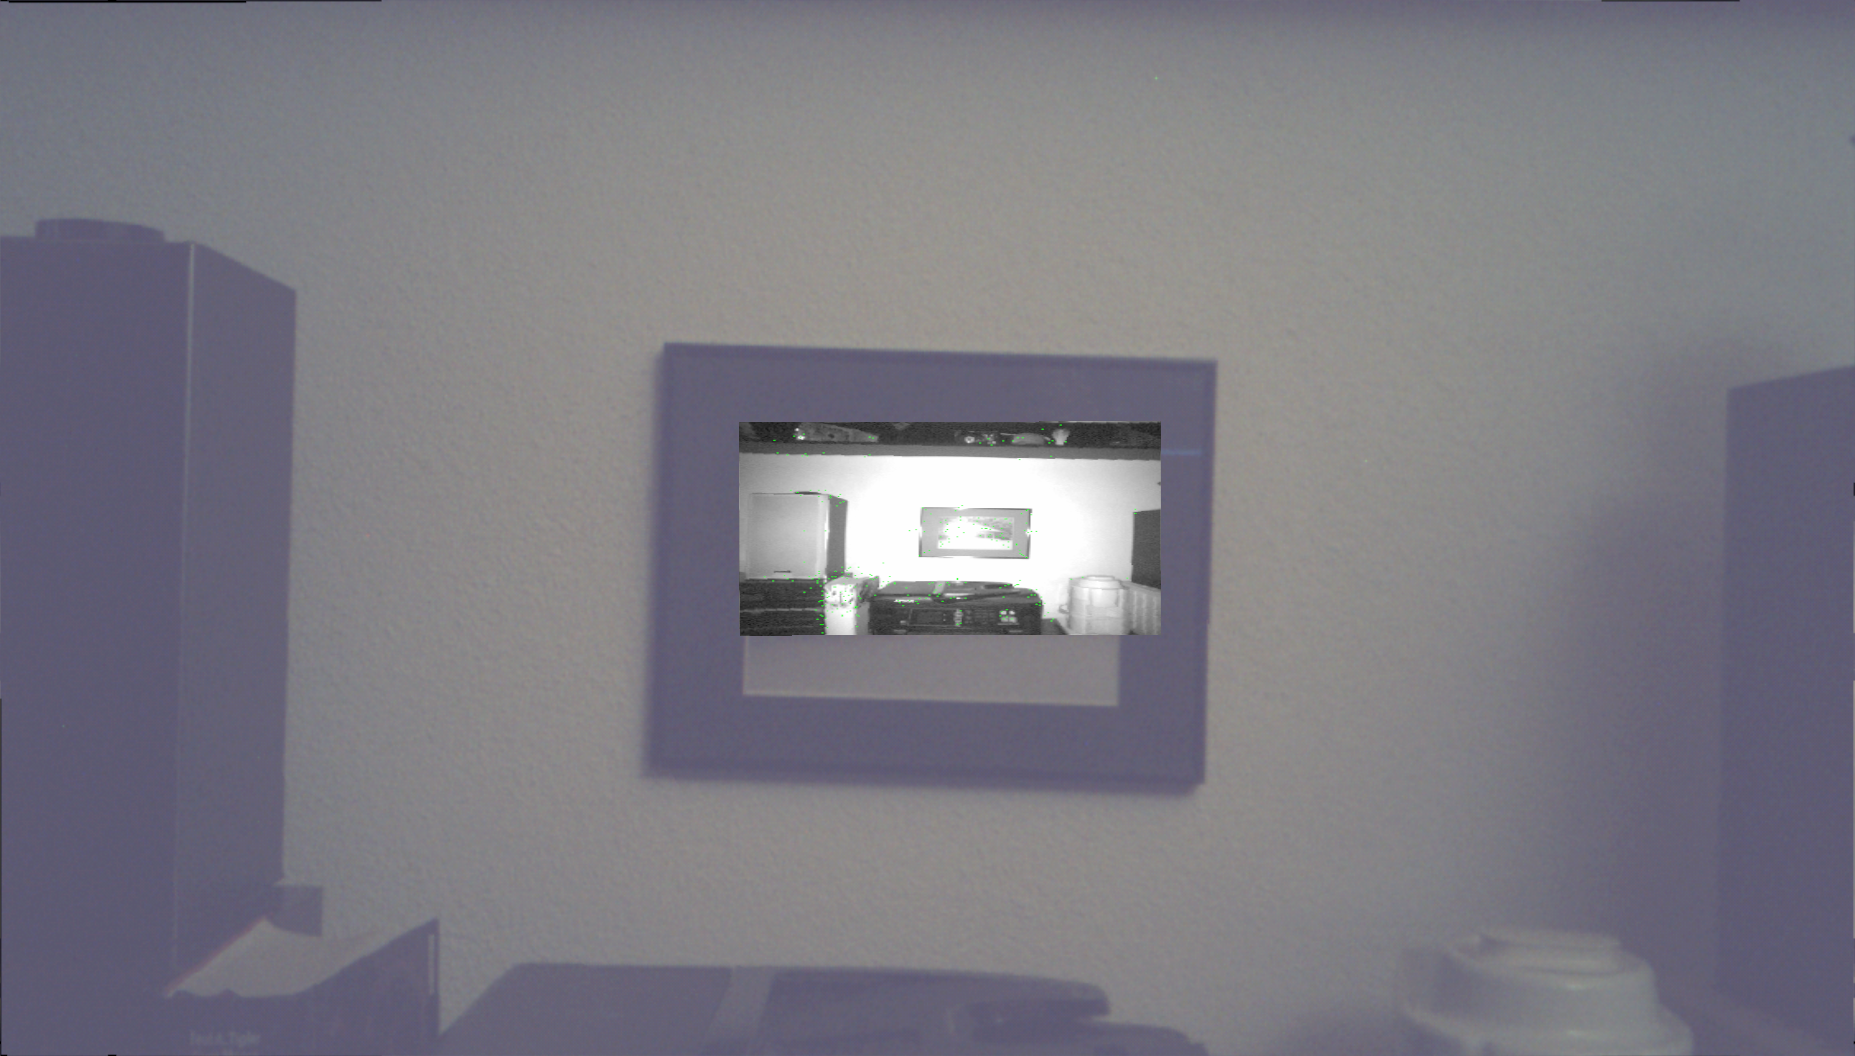
\includegraphics[scale=0.1115]{images/demo_rotation_init.png}
    \subcaption{Initial situation}
    \label{fig:rotation_demo_init} 
  \end{minipage} % Hier darf keine Leerzeile zwischen den beiden Minipages liegen!
  \begin{minipage}[b]{0.47\textwidth}
    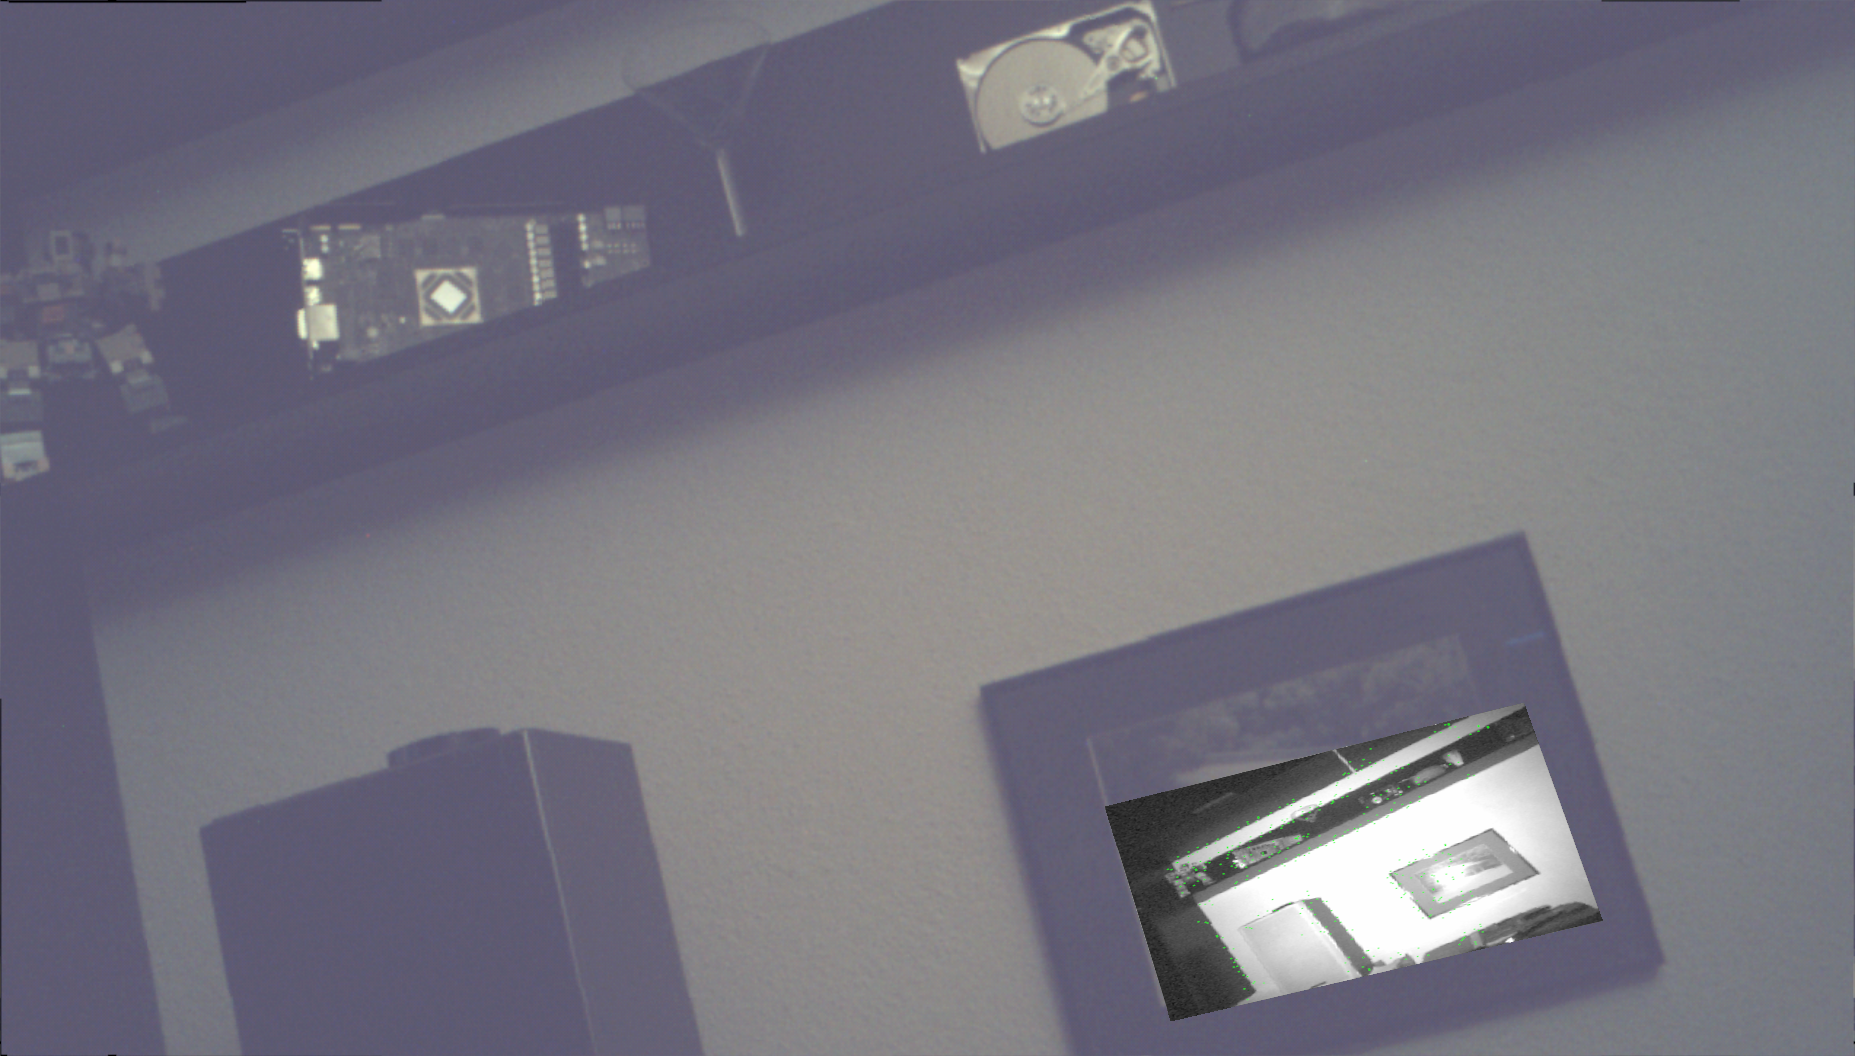
\includegraphics[scale=0.1115]{images/demo_rotation_rotated.png} 
    \subcaption{After rotation}
    \label{fig:rotation_demo_rotated} 
  \end{minipage}
  \caption{Demonstration of the rotation against the camera image with the moving projection. The displacement of the rectangle inside the picture frame is a result of the Raspberry Pi camera facing translational motion when rotated on the camera tripod.}
  \label{fig:rotation_demo}
\end{figure}
\subsection{Translation}
\label{sec:kalman_translation_results}
 Figure \ref{im:meas_kalman_translation} shows the output of the Kalman filter in green against the data from the accelerometer and the ToF camera. Without other input to compare against, the Kalman filter follows the accelerometer directly. The accelerometer's integration curve compares directly against the raw ToF camera data and the Kalman filter output on the velocity. Further integration allows the comparison with the positional data.\\
The accelerometer impacts the filter output, rendering it worse than the raw integration of the ToF camera. The Kalman velocity output is significantly worse than in the simulation, the proposed integration on this output, to get even better positional data fails.
\begin{figure}[H]
  \centering
  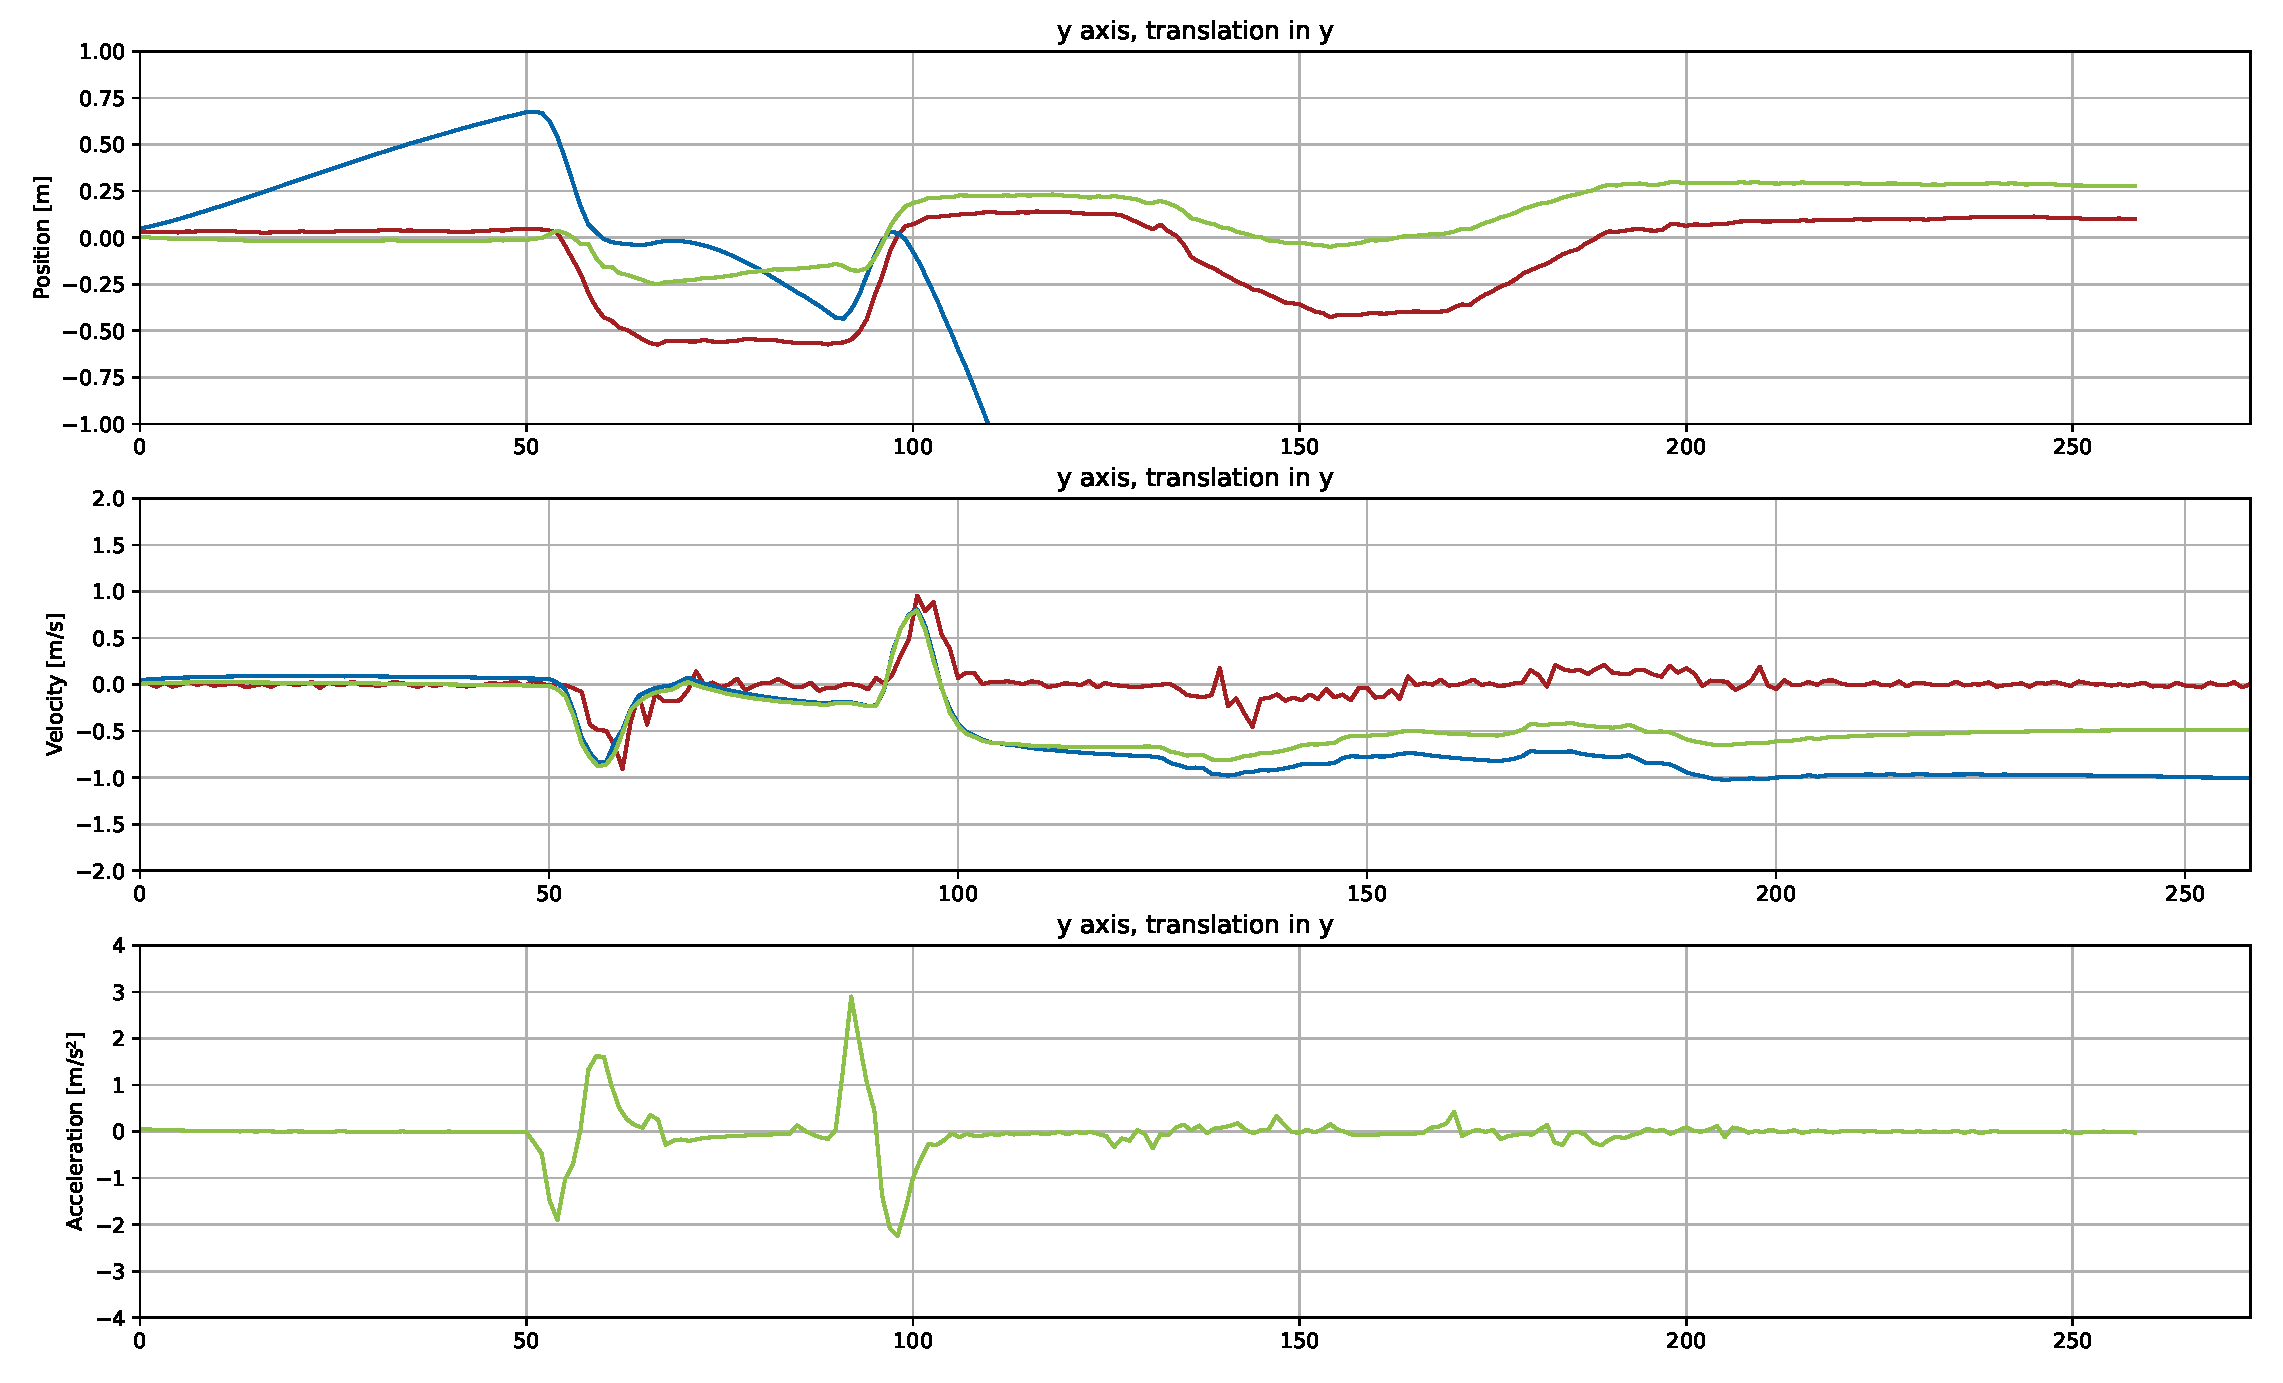
\includegraphics[width=1.0\textwidth]{images/measurement_kalman_translation.eps}
  \caption{Motion in y direction. Blue lines are data from the accelerometer and its integrations, red are the velocity from the ToF camera and its integration and in green are the different Kalman outputs. }
  \label{im:meas_kalman_translation}
\end{figure} 

%!TEX root = ../doc.tex
\chapter{Conclusion}
\label{sec:Conclusion}
The thesis shows that extracting rotation and translation speed from a ToF camera on a frame-by-frame basis works. The reconstruction of the three-dimensional scene from the depth image and SIFT feature points and running up to 512 parallel singular value transforms on brute-forced matches allows finding a good rotation and translation transform. This first step of the three-dimensional RANSAC algorithm enables the system to improve the matching quality by over a factor of two, compared to the brute-force matcher. Applying the singular value transform to each improved match results in an optimal rigid motion transform.\\
The noise of the ToF camera was a significant struggle during this thesis. The noise of the grayscale image causes the extracted SIFT features to jitter, even when the camera is stationary. The noise of the depth information increases the error on the three-dimensional scene reconstruction that forces the RANSAC algorithm to run with loose constraints. These loose constraints allow the RANSAC algorithm to falsely match features only because they are close enough, which induces an error on the rotation and translation estimation. This error again causes the motion data to be noisy.\\
The low framerate of the ToF camera and the processing pipeline is a problem for the Kalman filter, which cannot run at higher speeds. The frame-by-frame translation and rotation information is an average of the motion between the frames, not the velocity at the current frame's time. The low sampling rate requires a downsampling of the IMU data, which induces problems with the gravity compensation.\\ 
The system relies on finding SIFT features on its grayscale image – the algorithm will possibly not find enough features in an empty room.


\section{Possible improvement}
\label{sec:improvement}
A system that estimates the position directly based on visual key points is required to avoid drift on the rigid motion. A visual key point might be a specific cloud of SIFT features or an object classified by an ML algorithm.\\
The system would need to detect new key points, store them in a list, store the position and maybe even improve its position information when new data is available. Estimating the camera's position becomes possible from the external objects' position.\\
The position estimation from an image is valid for the moment where the frame got recorded – unlike the velocity, which is an average between two images. Therefore, the position estimation is not required to run at a high frame rate.\\
A different sensor fusion approach, which allows the IMU to run at its sampling rate without requiring a cumulative sum, would improve the position estimation. The orientation of gravity could be estimated at any point and could correct every single accelerometer measurement.
 

\section{Outlook}
\label{sec:outlook}
Augmented Reality is a vast field with various problems that need to be solved. The moment motion tracking works reliably, it enables multiple applications. Increasing the frame rate and accuracy with a better ToF sensor, as currently investigated by the Institute of Signal Processing and Wireless Communications of ZHAW, might enable the system for other topics. Motion tracking by a ToF camera might be implemented in an autonomous driving platform, with a custom-tailored Kalman filter that takes the wheels and steering into account.\\ 
Developing specialized hardware would be a larger project, as this involves many technologies, like optics, eye tracking, translucent displays and a portable processing platform.\\
Projecting outwards, the author expects Augmented Reality goggles for end consumers to hit the market within the following years, possibly having a similar impact as the smartphone once had. 
 

% Generate title for lists
\cleardoublepage
\phantomsection
\addcontentsline{toc}{chapter}{Verzeichnisse}

% Generate the bibliography and add it to the table of contents, there is an extra bib file where you can add entries(subfolder BibTeX-Literaturverzeichnis)
\cleardoublepage
\phantomsection
\addcontentsline{toc}{section}{\bibname}
\bibliographystyle{unsrt}
\bibliography{BibTex/literatur}

% Additional lists
\cleardoublepage
\phantomsection
\addcontentsline{toc}{section}{\listfigurename}
\listoffigures

\cleardoublepage
\phantomsection
\addcontentsline{toc}{section}{\listtablename}
\listoftables

\ifdefined\USEGLOSSARIES
	\cleardoublepage
	\phantomsection
	\addcontentsline{toc}{section}{Akronyme}
	\printglossary[type=\acronymtype]
	
	\cleardoublepage
	\phantomsection
	\addcontentsline{toc}{section}{Glossar}
	\printglossary
\else
	\cleardoublepage
	\phantomsection
	\addcontentsline{toc}{section}{Abkürzungsverzeichnis}
	\chapter*{List of Abbreviations}\label{sec:Glossar}

\begin{longtable}{|m{3cm}|m{11cm}|}	
	\rowcolor{gray} \textbf{Abbreviation}&
	Meaning \\ \hline	
	
	\textbf{ZHAW}&
	Zurich University of Applied Sciences \\ \hline	
	
	\textbf{InES}&
	Institute of Embedded Systems \\ \hline
	
	\textbf{HPMM}&
	High Performance Multimedia - a research group ant ZHAW-InES \\ \hline

	\textbf{ToF}&
	time-of-flight \\ \hline
	
	\textbf{LiDaR}&
	Light-Detection and Ranging \\ \hline	

	\textbf{MEMS}&
	Microelectromechanical systems \\ \hline

	\textbf{IMU}&
	Inertial Measurement Unit, a sensor for acceleration, rotation and magnetic fields \\ \hline	

	\textbf{SVD}&
	Singular Value Decomposition \\ \hline

	\textbf{RANSAC}&
	Random Sample Consensus \\ \hline

	\textbf{SSD}&
	Sum of Square Differences \\ \hline

	\textbf{GLFW}&
	Graphics Library Framework \\ \hline

	\textbf{GLM}&
	Graphics Library Mathematics \\ \hline

	\textbf{OpenGL}&
	Open Graphics Library - Predecessor of Vulkan \\ \hline

	\textbf{CUDA}&
	Compute Unified Device Architecture - NVIDIAs General-purpose computation on GPU\\ \hline	
	
	\textbf{CSI2}&
	Camera Serial Interface 2 - Video input interface\\ \hline

	\textbf{V4L2}&
	Video for Linux 2 - Videostreaming framework on Linux\\ \hline

	\caption{List of Abbreviations}
	\label{tab:glossar}
\end{longtable}%

\fi

\cleardoublepage
\phantomsection
\addcontentsline{toc}{section}{Listings}


\chapter{Appendix}
\label{sec:Anhang}

\section{Structure of the Git-Repository}
\label{sec:Anhang_struktur}
\subsection{Documentation}
Contains this documentation and all the images needed to build it.
\subsection{Source}
Contains all the source code, subdivided in Folders for device drivers, middleware and userspace-software
\subsection{Literature}
Contains 3rd party documents for technologies used in this thesis

\section{Used software}
\label{sec:usedSoftware}
The following software has been used for this thesis:
\begin{itemize} %
	\item Visual Studio Code: Software development on Linux, Jupyter-Notebooks for simulation and LaTeX for this documentation.
	\item Python 3.8 - with the Python-Plugin for VS Code.
	\item MikTex - with the LaTeX-Workshop-Plugin for VS Code.
	\item Adobe Illustrator 2021: Creating visuals for this documentation
	\item Adobe Photoshop 2021: Creating visuals for this documentation
	\item Grammarly Premium: For spellchecking this thesis
	\item Microsoft OneNote: As a notepad
	\item Microsoft Excel: For evaluation of the benchmarks
	\item NVIDIA JetPack 4.4: For flashing the TX2 and profiling the application
\end{itemize} % Anhang

\end{document}
